\documentclass[11pt]{article}
\ifdefined\pdfinfoomitdate\pdfinfoomitdate=1\fi
\ifdefined\pdftrailerid\pdftrailerid{}\fi
\ifdefined\pdfsuppressptexinfo\pdfsuppressptexinfo=15\fi
\usepackage[T1]{fontenc}
\usepackage{lmodern}
\usepackage[margin=1.08in]{geometry}
\usepackage{amsmath,amssymb,amsthm,mathtools,mathrsfs}
\usepackage{microtype,graphicx,booktabs,enumitem,flafter}
\usepackage{xcolor,tikz}
\usetikzlibrary{arrows.meta,positioning,calc,patterns}
\usepackage[numbers,sort&compress]{natbib}
\usepackage[colorlinks=true,linkcolor=teal!60!black,citecolor=teal!60!black,urlcolor=teal!60!black]{hyperref}
\usepackage[capitalize,nameinlink,noabbrev]{cleveref}
\hypersetup{pdftitle={The joint scaling limit of critical Ashkin-Teller currents},pdfauthor={OpenAI}}
\newtheorem{theorem}{Theorem}[section]
\newtheorem{proposition}[theorem]{Proposition}
\newtheorem{lemma}[theorem]{Lemma}
\newtheorem{corollary}[theorem]{Corollary}
\theoremstyle{definition}
\newtheorem{definition}[theorem]{Definition}
\newtheorem{remark}[theorem]{Remark}
\newtheorem{convention}[theorem]{Convention}
\crefname{equation}{Equation}{Equations}
\crefname{section}{Section}{Sections}
\newcommand{\R}{\mathbb R}
\newcommand{\Z}{\mathbb Z}
\newcommand{\N}{\mathbb N}
\newcommand{\E}{\mathbb E}
\renewcommand{\P}{\mathbb P}
\newcommand{\dd}{\,\mathrm d}
\newcommand{\eps}{\varepsilon}
\newcommand{\ind}{\mathbf 1}
\newcommand{\GFF}{\mathrm{GFF}}
\newcommand{\CLE}{\mathrm{CLE}}
\newcommand{\FPS}{\mathrm{FPS}}
\DeclareMathOperator{\Var}{Var}
\DeclareMathOperator{\Cov}{Cov}
\DeclareMathOperator{\diam}{diam}
\DeclareMathOperator{\dist}{dist}
\DeclareMathOperator{\supp}{supp}
\DeclareMathOperator{\Law}{Law}
\DeclareMathOperator{\sgn}{sgn}
\newcommand{\cA}{\mathcal A}
\newcommand{\cC}{\mathcal C}
\newcommand{\cF}{\mathcal F}
\newcommand{\cH}{\mathcal H}
\newcommand{\TVS}[2]{A_{-#1,#2}}
\numberwithin{equation}{section}
\setlist{itemsep=3pt,topsep=5pt}
\setlength{\emergencystretch}{2em}
\title{The joint scaling limit of critical Ashkin--Teller currents}
\author{OpenAI}
\date{September 25, 2026}
\begin{document}
\maketitle
\begin{abstract}
For each fixed point on the critical Ashkin--Teller line, including the
four-state Potts endpoint, we prove the conjectured joint scaling limit
of the height and both current-cluster collections in every bounded
Jordan domain, for every admissible polygonal approximation. The height
converges to a Gaussian free field with the predicted coupling constant,
and the clusters converge to canonical recursive two-valued local sets
of that same field. The joint limit includes all nesting depths and the
distinguished wired boundary cluster.
\end{abstract}
\tableofcontents
\section{Introduction}\label{sec:introduction}

The Ashkin--Teller model originates in the four-component lattice model
of Ashkin and Teller \cite{AshkinTeller1943}. Its current representation
raises a geometric question beyond convergence of the associated height:
what is the joint continuum law of all primal and dual current clusters,
and how are these collections coupled to the field? We prove the joint
limit in \cref{thm:main} for every fixed point on the critical line,
including the four-state Potts endpoint. This is the height and
current-cluster assertion formulated by Alcalde L\'opez, Heeney, and Lis
\cite[Conjecture~1.2]{AlcaldeLopezHeeneyLis2026}.

Fix $J>0$ and $U\le J$ with $\sinh(2J)=e^{-2U}$. Our zero-boundary
Gaussian free field has covariance $2\pi(-\Delta_D)^{-1}$, with
logarithmic singularity $-\log|z-w|$. In this normalization put
\[
 \lambda=\frac\pi2,\qquad a=\lambda\sqrt g,\qquad
 g=\frac8\pi\arcsin\!\left(\frac{\sqrt{1+e^{4U}}}{2}\right).
\]
Thus $4/3<g\le4$ and $\lambda<a\le2\lambda$. For the wired current,
the first limiting cluster is the symmetric two-valued local set with
labels $\pm a$. For the free current, first expose $\CLE_4$ holes and
retain an asymmetric two-valued split inside each hole; repeat in all
complementary components. Both constructions use the same field.
The theorem retains every nesting depth and the distinguished wired
boundary cluster. It includes tightness and identification of the entire
compact supports in positive-diameter Hausdorff matching topology.

\subsection*{Prior work and the scope of the result}
The finite spin, percolation, and height representation used here is due
to Lis \cite[Sections~1.1--1.3 and~2.2]{Lis2022Spins}; his current expansion
\cite[Section~2]{Lis2022Boundary} gives the precise odd/even-edge weights.
A noncrossing primal--dual contour representation appears earlier in Rys
\cite[Section~3]{Rys1963}. We recall and verify the finite coupling,
including its boundary convention, in \cref{sec:model}.

At $U=0$, the currents are double random currents and $g=2$.
Duminil-Copin and Lis \cite[Theorems~1.1--1.2]{DuminilCopinLis2019}
identified the finite signed nesting field with a dimer height.
Duminil-Copin, Lis, and Qian \cite{DRC2025} established conformally
invariant limits for the nesting field and recursive cluster-boundary
families. Their introductory statements cover Jordan domains, while the
detailed joint boundary-family Theorems~6.2 and~6.4 assume a $C^1$
boundary and use injective matching of loops. Alcalde L\'opez, Heeney,
and Lis \cite[Theorem~1.14 and Appendix~B]{AlcaldeLopezHeeneyLis2026}
state the joint limit of the height and both complete compact
current-cluster collections in Jordan domains, using the noninjective
positive-diameter matching topology considered here. Their
Conjecture~1.2 asks for the critical-line extension obtained by replacing
$\sqrt2$ with $\sqrt g$.

Alcalde L\'opez and Sep\'ulveda
\cite[Theorems~1.4 and~9.5, and Lemma~9.1]{AlcaldeLopezSepulveda2026} study a stronger
joint decomposition at the Ising point involving the XOR field, cluster
measures, and signs, with the Gaussian field identified with the nesting
height. Their introductory theorem is stated for Jordan domains; their
detailed joint convergence theorem adds a boundary Minkowski-dimension
hypothesis. Those additional field and measure limits are
outside our statement. Our conclusion concerns the height and complete
current supports for every fixed $4/3<g\le4$.

The analytic input is related to the six-vertex model with weights
$(1,1,c)$, where $c=\sqrt{1+e^{4U}}\in(1,2]$.
Duminil-Copin, Kozlowski, Lammers, and Manolescu \cite{DKLM2026}
prove a height scaling limit for $\sqrt3\le c\le2$ and establish several
inputs on the larger interval $1\le c\le2$: logarithmic bounds for even
increment moments, one-parity spin-percolation circuits, a specified
flat-exhaustion plane law, and a free-energy identification of the
normalization conditional on a Gaussian plane limit. Odd plane correlations
vanish by height reversal. We use these larger-range results. The covariance, screening,
and Gaussianity arguments needed for the whole interval are given here;
the free-energy formula is applied only after its convergence premise
has been established. A related full-plane height theorem for the balanced
six-vertex state is proved in \cite[Theorem~1.1]{BalancedSixVertex2026}. Its unit
height corresponds to $K=2H$ here, and its multiplier
$1/\arcsin(c/2)$ agrees with ours after this normalization. This
comparison does not replace the local Gaussianity proof or the
random-domain and cluster identifications below.

For the reflection argument, coordinate and diagonal tests for
six-vertex weights already appear in
\cite[Section~6]{FrohlichIsraelLiebSimon1980}. We use the general
reflection-positive framework of \cite{FrohlichIsraelLiebSimon1978};
for the reflected Hilbert-space construction and positive-transfer
representation, see \cite[Sections~3.1--3.3 and~4.1]{Usui2012}.
The height transfer in \cite[Section~4.5.3]{DKLM2026} is a closer
model-specific precedent and permits negative one-step spectrum.
The transfer, screening, and collision strategy also has a related
implementation for integer Lipschitz heights with two-arc boundary data
in \cite[Sections~5, 7, and~9--10]{Triangular}. We prove the square-frame
and random-chamber arguments required here.

The continuum identification uses thin two-valued local sets
\cite{ASW2017,AS2018}, first-passage sets \cite{ALS2017,ALS2018}, and
the canonical excursion decomposition \cite{ALS2023}. The recursive
exploration and thinness architecture also follows the double-current
work \cite{DRC2025}. In the present coupling, we must additionally
identify which discrete odd holes belong to a single current cluster,
exclude macroscopic pieces invisible to those holes, and compare passage
tests after a second coupled random exploration. We prove these steps
with the conditioning and approximation hypotheses stated in the
corresponding propositions. A proof strategy follows the formal theorem
in \cref{subsec:proof-strategy}.

\section{The model and the limiting objects}\label{sec:model}

\subsection{Parameters and lattice domains}\label{sec:lattice-domains}
Fix real numbers \(J>0\) and \(U\leq J\) satisfying
\[
 \sinh(2J)=e^{-2U}.
\]
Throughout the proof these parameters remain fixed. Put
\begin{equation}\label{eq:parameters}
 t=(1+e^{4U})^{-1/2},\qquad c=t^{-1},\qquad
 \theta=\arcsin(c/2),\qquad g=\frac{8\theta}{\pi}.
\end{equation}
Then \(1/2\leq t<1\), \(1<c\leq2\), and \(4/3<g\leq4\).
The value \(U=0\) gives \(g=2\); the endpoint
\(J=U=(\log3)/4\) gives \(g=4\). Constants below may depend on the
fixed parameter. We make no claim of uniformity as \(t\uparrow1\).

Let \(D\subset\R^2\) be a bounded Jordan domain. An admissible approximation
is a family of simple nearest-neighbor polygons \(P_\delta\) in
\(\delta\Z^2\) such that their boundaries have parametrizations converging
uniformly to a parametrization of \(\partial D\), and every compact subset
of \(D\) eventually lies inside \(P_\delta\).
Let \(G_\delta=(V_\delta,E_\delta)\) contain all lattice vertices and edges
on or inside the polygon, and let \(B_\delta\) be its boundary-cycle edges.
The weak dual \(G_\delta^\dagger\) has a vertex at each bounded-face center
and an edge across each edge of \(E_\delta\setminus B_\delta\).
We draw all primal and dual edges as straight segments. Boundary
contraction will be used only to describe current weights, not when
drawing clusters.

\subsection{The coupled currents and their height}
We use the spin--edge--height construction of
\cite[Sections~1.1--1.3]{Lis2022Spins}, with its wired/free boundary
specialization made explicit below. Sample spins
\[
 \tau:V_\delta\longrightarrow\{-1,1\},\qquad
 \tau^\dagger:V(G_\delta^\dagger)\longrightarrow\{-1,1\},
\]
with \(\tau=1\) on \(P_\delta\). For each mutually dual pair
\(e=uv\), \(e^\dagger=ff'\), impose
\begin{equation}\label{eq:spin-constraint}
 (\tau(u)-\tau(v))(\tau^\dagger(f)-\tau^\dagger(f'))=0.
\end{equation}
Give an admissible pair weight
\begin{equation}\label{eq:spin-weight}
 t^{N(\tau)+N(\tau^\dagger)},
\end{equation}
where \(N\) counts nearest-neighbor disagreements on the respective
graph. No boundary constraint is imposed on the dual spins.

Conditional on the spins, all edges of \(B_\delta\) are primal open.
For each remaining mutually dual pair, independently of the other pairs,
use the following rule:
\begin{center}
\begin{tabular}{@{}lll@{}}
\toprule
Spin information & Primal/dual open states & Probabilities\\
\midrule
\(\tau^\dagger(f)\ne\tau^\dagger(f')\) & \((1,0)\) & \(1\)\\
\(\tau(u)\ne\tau(v)\) & \((0,1)\) & \(1\)\\
Neither disagreement & \((1,0),(0,1),(0,0)\) & \(1-t,1-t,2t-1\)\\
\bottomrule
\end{tabular}
\end{center}
The constraint makes the first two rows mutually exclusive.
Denote the resulting edge sets by
\(\widehat n_\delta\) and \(\widehat n_\delta^\dagger\).
Their open edges never cross. Both may be closed at a mutually dual pair;
the two currents are not generally complementary.

After contracting the wired boundary and deleting its cycle edges, the
primal odd edges are those crossing dual spin disagreements. The other
primal open edges are even. In the current expansion of
\cite[Section~2, Equations~(2)--(3) and Proposition~1]{Lis2022Boundary},
their law specializes to
\begin{equation}\label{eq:current-weight}
 \P(n_{\rm odd},n_{\rm even})\ \propto\
 2^{k(n_{\rm odd}\cup n_{\rm even})}
 x^{|n_{\rm odd}|}y^{|n_{\rm even}|},
 \qquad
 x=1,\quad y=c-1,
\end{equation}
with \(n_{\rm odd}\) Eulerian and disjoint from \(n_{\rm even}\).
Here \(k\) includes isolated vertices. To check the weight directly,
an odd edge contributes \(t\), an even edge contributes \(1-t\),
and a closed primal edge contributes \(t\), after summing its possible
dual states. The common factor is \(t^{|E_\delta\setminus B_\delta|}\),
leaving \(((1-t)/t)^{|n_{\rm even}|}\).
The primal colors are constant on open components and give
\(2^{k-1}\) choices with the wired color fixed. An admissible Eulerian
odd set determines the dual colors up to a common flip.
These graph-dependent constant factors yield \cref{eq:current-weight}.
The same calculation gives free boundary conditions for the dual current.
In the original parameters,
\[
 x=e^{2U}\sinh(2J)=1,\qquad
 y=e^{2U}\cosh(2J)-1=\sqrt{1+e^{4U}}-1.
\]
It is the spin-and-edge construction above, not just
\cref{eq:current-weight}, that specifies the joint law.

Set \(H_\delta=0\) on \(P_\delta\), and define corner increments by
\begin{equation}\label{eq:height-increments}
 H_\delta(f)-H_\delta(v)=\frac12\tau(v)\tau^\dagger(f)
 \quad\text{when \(v\) is incident to \(f\)}.
\end{equation}
The circulation around an interior primal edge is
\[
 \frac12(\tau(u)-\tau(v))
              (\tau^\dagger(f)-\tau^\dagger(f'))=0.
\]
All boundary primal increments are zero. Since the polygon is simple,
these elementary circuits generate the corner graph's cycle space,
so \cref{eq:height-increments} defines a unique height.
It is integer-valued on primal vertices and half-integer-valued at face
centers. We also use
\[
 K_\delta=2H_\delta.
\]
Thus a nearest corner increment of \(K_\delta\) has magnitude one.
Conversely, the spins are recovered from its residues, up to a common
sign \(\varepsilon\), by
\[
 \tau(v)=\varepsilon(-1)^{K_\delta(v)/2},\qquad
 \tau^\dagger(f)=\varepsilon(-1)^{(K_\delta(f)-1)/2}.
\]
Around a corner-lattice plaquette there are six possible increment
patterns. The two patterns with both opposite diagonals flat have spin
weight \(1\); the other four have weight \(t\). Dividing by the common
factor \(t\) gives the six-vertex weights \((1,1,c)\), with \(c=1/t\);
see also \cite[Section~2.2, Corollary~2.5]{Lis2022Spins}.
The corner lattice is a fixed rotation and dilation of the square
lattice. This local identification, together with the infinite-volume
identification recalled in \cref{sec:spectral}, is what permits the
six-vertex estimates used below.
As a distribution on \(D\), the height is
\begin{equation}\label{eq:height-smearing}
 H_\delta(\varphi)=\delta^2
       \sum_{v\in V_\delta}H_\delta(v)\varphi(v),
 \qquad \varphi\in C_c^\infty(D).
\end{equation}
This is an atomic distribution, which belongs locally to \(H^s\) for
\(s<-1\). Interpolated heights used in intermediate estimates will be
compared with this precise smearing.

Let \(\cC_\delta^{\rm w}\) be the collection of all connected components
of the primal open subgraph, including its boundary component
\(C_{\partial,\delta}\), and let \(\cC_\delta^{\rm f}\) be the collection
of all dual open components. A component includes its vertices and drawn
edges. We retain components at every nesting depth.

\subsection{An auxiliary representation}\label{subsec:auxiliary}
When analyzing one of the two currents, denote it by \(N\), and denote
its exact dual complement by \(W\). This complement is an auxiliary
spin percolation, not the other current of the joint sample.
The spin constant along \(W\) is called \(s\), and the spin constant
along \(N\) is called \(d\). At an ambiguous pair, \(W\) is open with
probability \(t\), whereas the other current is open with probability
\(1-t\).

A \emph{matching wall} means a revealed monochromatic open path or
perimeter in the \(W\)-lattice. Its connections in the revealed region
are retained as boundary connections; separate appearances of the same
connected perimeter are not treated as unrelated wires.
For a free current, the complementary \(W\)-percolation is wired.
The finite cut law in \cref{lem:finite-cuts} explains why the height in
a component behind a matching wall has constant boundary data.
All conditional comparisons below refer to this representation.

The same cut law gives the vocabulary for nesting. A hole of a free
\(N\) component is \emph{odd} when its adjacent \(s\) spin differs from
the adjacent exterior \(s\) spin of that component. Crossing the component
changes \(K_\delta\) by \(2\) times one relative sign in every odd hole,
and by zero in every other hole. Conditional on \((N,s)\), these signs
are independent and fair for distinct free components. After the wired
boundary component is exposed, each residual chamber carries a free
same-parity current; the value of \(K_\delta\) on its component-side
\(W\) perimeter is \(+1\) or \(-1\)
relative to the original boundary height. The edge factor and the jump
identity proving these statements are given in \cref{lem:finite-cuts}.

\subsection{Continuum normalization and two-valued sets}
Let \(h\) be the zero-Dirichlet GFF in \(D\) with covariance
\[
 G_D=2\pi(-\Delta_D)^{-1}.
\]
Thus \(G_D(z,w)=-\log|z-w|+O(1)\) near the diagonal. Set
\begin{equation}\label{eq:normalization}
 \lambda=\frac{\pi}{2},\qquad
 a=\sqrt g\,\lambda,\qquad
 a^2=2\pi\arcsin(c/2).
\end{equation}
In particular \(\pi/\sqrt3<a\leq\pi\), so
\(\lambda<a\leq2\lambda\). A zero-boundary GFF in an open subdomain is
always extended by zero when viewed as a distribution on a larger
domain.

We use the canonical thin two-valued local set
\(\TVS{\alpha}{\beta}(f)\) of a zero-boundary GFF \(f\), with
\(\alpha,\beta>0\) and \(\alpha+\beta\geq2\lambda\). It includes the domain boundary.
The conditional harmonic function on each complementary component is
either \(-\alpha\) or \(\beta\); after subtracting that value, the field in the
component is an independent zero-boundary GFF. These sets are measurable
functions of the field. We use their uniqueness, monotonicity, and
Jordan-hole properties with the hypotheses stated in
\cref{sec:local-sets}; see \cite{ASW2017,AS2018,ALS2017}.
In particular the complementary loops of
\(\TVS{2\lambda}{2\lambda}\) have law \(\CLE_4\).

\begin{definition}[Free cluster procedure]\label{def:free-procedure}
For a zero-boundary GFF \(f\) in a Jordan domain \(O\), define
\(\mathcal F_a(f,O)\) recursively as follows.
\begin{enumerate}
\item Expose \(\TVS{2\lambda}{2\lambda}(f)\). In every complementary
component \(V\), write its label as \(\xi\,2\lambda\),
\(\xi\in\{-1,1\}\), and let \(f_V\) be the zero-boundary remainder.
\item If \(\xi=1\), retain
\(\TVS{2\lambda}{2a-2\lambda}(f_V)\) as one cluster. If \(\xi=-1\),
retain \(\TVS{(2a-2\lambda)}{2\lambda}(f_V)\).
The retained set includes its outer boundary \(\partial V\).
\item In each complementary component of the retained set, subtract its
conditional harmonic value and repeat the procedure with the
zero-boundary remainder.
\end{enumerate}
Keep all retained clusters from all recursive generations. The
\(\CLE_4\) set exposed in the first step is not itself retained.
\end{definition}

If this procedure is invoked above an incoming flat value \(b\) of the
original field, the CLE component has absolute label \(b+\xi2\lambda\)
and the retained split has absolute labels \(b\) and \(b+\xi2a\).
We call the holes with the nonzero jump relative to this incoming value
\(b\) \emph{odd holes}.
The use of this term in lattice explorations is consistent with the
jump decomposition proved below.

Define
\[
 \cC^{\rm f}=\mathcal F_a(h,D).
\]
For the wired collection, first retain
\[
 C_\partial=\TVS{a}{a}(h),
\]
and apply \(\mathcal F_a\) to the zero-boundary remainder in every
complementary component of \(C_\partial\), retaining all resulting
clusters together with \(C_\partial\). Denote that collection by
\(\cC^{\rm w}\). Both constructions use the \emph{same} \(h\), including
the canonical choices of all its local sets. This defines their joint
coupling. The all-generation local finiteness needed below is proved
in \cref{cor:canonical-local-finiteness}, rather than assumed as part of the
definition.

\begin{figure}[!htbp]
\centering
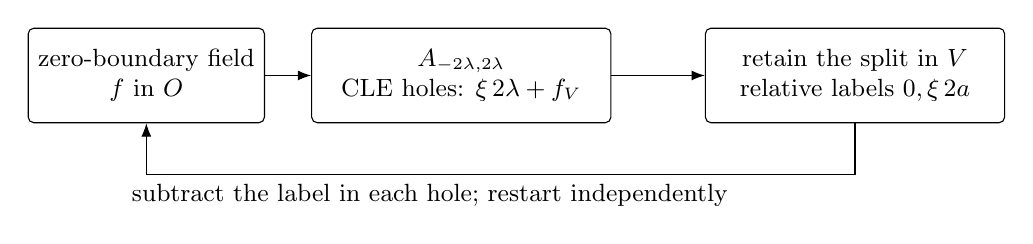
\begin{tikzpicture}[font=\small,>=Latex]
 \node[draw,rounded corners=2pt,align=center,minimum width=30mm,
       minimum height=12mm] (f) at (0,0) {zero-boundary field\\\(f\) in \(O\)};
 \node[draw,rounded corners=2pt,align=center,minimum width=38mm,
       minimum height=12mm] (cle) at (4,0)
       {\(\TVS{2\lambda}{2\lambda}\)\\CLE holes: \(\xi\,2\lambda+f_V\)};
 \node[draw,rounded corners=2pt,align=center,minimum width=38mm,
       minimum height=12mm] (split) at (9,0)
       {retain the split in \(V\)\\relative labels \(0,\xi\,2a\)};
 \draw[->] (f)--(cle);
 \draw[->] (cle)--(split);
 \draw[->] (split.south)--++(0,-.65)-|
       node[pos=.3,below,align=center]
       {subtract the label in each hole; restart independently} (f.south);
\end{tikzpicture}
\caption{One recursive step of the free construction. Only the split
inside a CLE hole is retained as a current cluster. For the wired
construction, the boundary set \(\TVS{a}{a}\) is retained first.}
\label{fig:free-procedure}
\end{figure}

\subsection{Topology and the theorem}
Fix a compact square \(X\) containing \(\overline D\) and all sufficiently
fine polygonal approximations. Such a square exists by admissibility.
Let \(\mathscr H=\mathcal K(X)\) be the space of nonempty compact subsets
of \(X\), with Hausdorff metric \(d_H\), and let
\(Z=\{\{x\}:x\in X\}\subset\mathscr H\) be its singleton subspace.
A collection \(\mathcal K\subset\mathscr H\) is locally finite above
positive diameter if
\[
 \#\{C\in\mathcal K:\diam(C)>\eps\}<\infty
 \qquad\text{for every \(\eps>0\)}.
\]
For such a collection put
\[
 F(\mathcal K)=Z\cup\{C\in\mathcal K:\diam(C)>0\},\qquad
 d_{\rm match}(\mathcal K,\mathcal K')
   =d_H^{\mathscr H}\bigl(F(\mathcal K),F(\mathcal K')\bigr),
\]
where \(d_H^{\mathscr H}\) is Hausdorff distance between compact subsets
of \(\mathscr H\). Local finiteness makes \(F(\mathcal K)\) closed:
any convergent sequence of distinct members has diameters tending to
zero and therefore has a singleton limit. Thus \(d_{\rm match}\) is a
metric after singleton members and multiplicities are ignored.

This metric gives precisely the positive-diameter matching topology.
To make the relation with the usual description explicit, write
\(R_\eps(\mathcal K,\mathcal K')\) for the following two requirements:
\begin{align*}
 &\text{every \(C\in\mathcal K\) with \(\diam(C)>\eps\) has some
 \(C'\in\mathcal K'\) with \(d_H(C,C')<\eps\),}\\
 &\text{and the same statement holds with \(\mathcal K,\mathcal K'\)
 interchanged.}
\end{align*}
The matching need not be one-to-one. We retain the distinguished boundary
component separately, with ordinary Hausdorff topology.

\begin{lemma}[Matching topology and compact containment]
\label{lem:matching-topology}
As relations on locally finite collections,
\[
 \{d_{\rm match}\le\eps/2\}\subset R_\eps
       \subset\{d_{\rm match}\le\eps\}.
\]
Let \(\mathfrak X\) be the compact space of closed subsets
\(F\subset\mathscr H\) containing \(Z\), and write
\(N_t(F)=\#\{C\in F:\diam(C)>t\}\). If \(t_j\downarrow0\) and every
\(M_j\) is finite, then
\[
 \{F\in\mathfrak X:N_{t_j}(F)\le M_j\text{ for every }j\}
\]
is compact and consists of locally finite collections after singleton
members are removed. Consequently, uniform tails for \(N_t\) at each
fixed \(t>0\) imply compact containment in the matching topology.
\end{lemma}

\begin{proof}
For every \(C\in\mathscr H\),
\[
 \frac12\diam(C)\le \dist_{\mathscr H}(C,Z)\le\diam(C).
\]
The lower bound is the triangle inequality, and the upper bound follows
by choosing a singleton in \(C\). If \(d_{\rm match}\le\eps/2\), a member
of diameter greater than \(\eps\) must therefore match a positive-diameter
member of the other family within \(\eps/2\). Conversely, under \(R_\eps\)
each member of diameter at most \(\eps\) is within \(\eps\) of \(Z\), and
each larger member has the required match. This proves the inclusions.

The hyperspace of nonempty compact subsets of a compact metric space is
compact, and the condition \(Z\subset F\) is closed. For each \(t>0\),
\(N_t\) is lower semicontinuous: any finitely many distinct members of
diameter greater than \(t\) persist in disjoint small hyperspace
neighborhoods under Hausdorff convergence. Hence each constraint
\(N_{t_j}\le M_j\) is closed. Their intersection is compact, and choosing
\(j\) with \(t_j<t\) proves finiteness above every \(t>0\). Finally, choose
the \(M_j\) so that the respective tail probabilities are at most
\(\eta2^{-j}\), and use the union bound. This proves compact containment.
\end{proof}

\begin{theorem}[Joint critical-line limit]\label{thm:main}
For every fixed pair $J>0$, $U\le J$ with $\sinh(2J)=e^{-2U}$,
every bounded Jordan domain $D$, and every admissible polygonal
approximation as defined in \cref{sec:lattice-domains},
\[
 \bigl(H_\delta,\cC_\delta^{\rm w},\cC_\delta^{\rm f},
                         C_{\partial,\delta}\bigr)
 \ \xrightarrow[\delta\downarrow0]{\mathrm{law}}\
 \left(\frac{h}{\pi\sqrt g},\cC^{\rm w},\cC^{\rm f},
                         \TVS{a}{a}(h)\right).
\]
The height converges in \(H^s_{\rm loc}(D)\) for every \(s<-1\).
Each cluster collection converges in the matching topology just
defined, and the distinguished component converges in Hausdorff
topology. The continuum collections are locally finite above every
positive diameter. All convergences are joint, and the same GFF
determines both continuum collections.
\end{theorem}

The height topology may equivalently be handled on a countable
exhaustion of \(D\) and a countable sequence of exponents increasing
to \(-1\). Our proof first obtains joint tightness, then identifies
every subsequential limit as the canonical construction of
\cref{thm:main}. This yields the full mesh limit without selecting a
preferred approximation sequence. No claim about cluster area measures,
magnetization fields, all spin-domain-wall curves, or an exact metric
exponent is part of the theorem.

\subsection{Stopping and limiting conventions}\label{subsec:conventions}
All lattice explorations reveal endpoint spins before prescribing an
edge. An accessible chamber keeps the actual boundary connections
created by the explored configuration. At a pinch, its boundary is the
perimeter walk on the side of that chamber; unrelated interiors are
not identified merely because their closures touch.

A \emph{pointed limiting component} is specified by a fixed interior
test point and compact subsets eventually contained in its discrete
component. Several such open components may arise from a single
discrete precursor. Statements about conditional fields in distinct
limiting components therefore include their joint independence after
the appropriate constants are removed. The needed uniform estimates
are established before local-set identification.

Geometric scales, buffers, and diameter thresholds are fixed before
letting \(\delta\downarrow0\). Subsequently a collar width or test scale
may tend to zero, and a finite-count truncation may be removed. Rational
polygons, rational balls, and a fixed countable dense family of interior
points make all uses of these limits simultaneous. Whenever a random
domain is used, its exact cut law specifies the residual boundary class.
An estimate for the residual fields may be invoked conditionally on the
stopping data when it is uniform over that class. Estimates controlling
the production of the cut itself are instead averaged over the exploration,
conditional only on the permitted initial flat data; they are not asserted
after conditioning on a completed stopping history.

\subsection{Proof strategy}\label{subsec:proof-strategy}
The proof first identifies the height field and then recovers the complete
current supports from the geometry coupled to that field.

\Cref{sec:spatial} fixes one current \(N\) and its complementary spin
percolation \(W\). The exact edge factor makes an open monochromatic
\(W\) perimeter a cut with a flat residual law. Ferromagnetic comparison
then supplies circuit estimates in the permitted residual states. The
collar argument controls long passages near a rough explored boundary by
summing bridge failures over the gaps between ordered crossings. It yields
macroscopic count tails and a no-shadowing estimate after a frozen indexed
stop. For a complete prescription of every \(s\) spin and \(W\) edge in a
small region, the pattern comparison compares its probability under allowed
exterior conditions with its plane probability, with a ratio bounded
independently of the number of microscopic prescriptions. A mixed-sign
witness argument then shows that full-spin events with vanishing plane
probability also have vanishing probability uniformly under the allowed flat
laws. This is the one-way contiguity used to transfer screening.

\Cref{sec:spectral} gives Cauchy-mixture representations of the plane
covariance in the four axial and diagonal reflection frames. At nonzero tangential
frequency \(k\), the normal Cauchy width \(s\) has defect
\(D(k,s)=((|k|-s)/(|k|+s))^2\). Fourth angular harmonics in frames differing
by \(45\) degrees cancel pointwise, making this defect integrable against
the mixing measure. For fixed \(0<b<B\), its integral on
\(b\delta\le|k|\le B\delta\) therefore tends to zero, so each rescaled
mixing limit is supported on \(s=|k|\).
Agreement in two independent frames then fixes the remaining spectral weight
in both directions, identifying the Green covariance without a
\(45\)-degree symmetry of the lattice law. In \cref{sec:screening}, the conditional mean of the neutral
Laplacian average \(K_\delta(\Delta\phi)\), given, outside a surrounding square,
both spin fields, the \(W\) states, and computable height increments, tends to zero in \(L^1\). This makes separated
limiting moments harmonic in \cref{sec:gaussian}. Logarithmic bounds then
exclude distributions supported on collision diagonals, and local neutral-pair
mixing identifies the logarithmic collision coefficients, giving Wick's rule.
For plane increment correlations the same argument gives compact-uniform
convergence at every order, which verifies the six-vertex convergence
criterion. Only after it yields the Gaussian plane limit does the free-energy
correspondence fix the coefficient.

\Cref{sec:local-sets} identifies random cuts. The discrete carpet obtained
by stopping each branch at its first odd jump converges to
\(\TVS{2a}{2a}\), which is distinct from a retained cluster of
\cref{def:free-procedure}. Exact finite cuts give independent flat laws in
the residual chambers. A neighborhood argument removes the contributions
of both the revealed mean and the centered remainder near the limiting cut.
Conditional characteristic functions then identify the full zero-extended
GFF remainder, while the piecewise constant labels give the full conditional
mean. This proves the thin local-set law for carpets and the localized
conditional decomposition away from the seed and the initial revealed wall
for cluster stops.
In \cref{sec:local-kernel},
strong convergence of Gaussian projections and cutoff Cameron--Martin
likelihoods give one local cable-test kernel shared by the canonical parent
and a separately stopped component. Testing the canonical forcing event
against the component's zero-boundary law shows that a canonical cluster in
the parent cannot meet both an unsearched stopped component and its boundary.

\Cref{sec:identification} uses this no-crossing result for one inclusion
of the visible partition: odd holes of one canonical cluster must come from
the same discrete precursor. The fair-sign correlation identity excludes a
precursor supplying holes of distinct canonical clusters. Finite witnesses
and the lattice count tails then prove local finiteness across all recursive
generations at once. To recover complete supports, we identify the full
conditional mean of a stopped exploration. An oscillatory GFF test excludes
a connected macroscopic cut where that mean is flat. The intersections of a
connected limiting precursor with the canonical supports and the initial wall
therefore form a countable pairwise disjoint closed cover. Sierpi\'nski's theorem
reduces this cover to one nonempty member. The rough-wall collar estimate
excludes the initial-wall case. The indexed no-shadowing estimate
and the discovery order exclude invisible duplicate precursors. This identifies
every subsequential limit and proves \cref{thm:main}.

\section{Cuts, comparison, and spatial estimates}
\label{sec:spatial}

In \crefrange{sec:spatial}{sec:gaussian}, heights are measured in the
normalization $K_\delta=2H_\delta$, whose nearest corner increments have
magnitude one.

The field limit needs control of local patterns, whereas the cluster
limit also needs estimates near the irregular boundaries left by an
exploration. We obtain both from one edge representation. Fix one of the
two currents and call it $N$. Let $W$ be its exact edge complement on the
other lattice: a $W$ edge is open precisely when the crossing $N$ edge is
closed. Write $s$ for the spin on the $W$ lattice and $d$ for the spin on
the $N$ lattice. Thus $W$ is monochromatic in $s$, while $N$ is
monochromatic in $d$. The graph $W$ is generally different from the other
current in the coupling. At an ambiguous edge its opening probability is
$t$, not $1-t$.

A \emph{flat chamber} means a component cut off by an open monochromatic
$W$ perimeter, with its height on that perimeter fixed. Boundary walks
may repeat vertices. At a pinch, the two incident faces on the unsearched
side remain separate unless they are actually connected there. One can
equivalently use medial boundary polygons displaced by one lattice unit
into the chamber. This convention changes Euclidean distances by
$O(\delta)$ and never joins two chambers across a pinch.

We use three kinds of conditional information. An \emph{exact cut
history} may contain the chosen current $N$, its colors, and the heights
on the revealed side of completed $W$ perimeters. The edge factor below
removes that information from every residual chamber. A comparison or
annular search \emph{inside} a residual chamber reveals only $(s,W)$,
and reveals an edge only after its endpoint spins. Finally, an auxiliary
matching fill changes the removed side of a cut for a geometric circuit
test; it is used through its accessible marginal and is not extra
conditioning of the original law. The edge decoration of the other
current has been summed out. It is never part of the stopping data on a
cut or on its unsearched side: conditioning it on an open $W$ edge can
restore an interaction between the transverse spins. Data strictly on an
already separated side may be retained by the exact cut factorization.

All constants below may depend on the fixed parameter $t\in[1/2,1)$ and
on stated macroscopic buffer ratios. They do not depend on the mesh,
on the number of microscopic edges of a prescribed pattern, or on the
length or number of fingers of a retained perimeter. In comparisons
involving several independently retained source wires, dependence on
their number will always be stated.

\subsection{Exact cuts and the comparison order}

\begin{lemma}[Finite cuts and colors]\label{lem:finite-cuts}
For every finite domain with either of the model's flat boundary
conditions, the joint weight of $(s,W,d)$ is a product
of the following factors, one for each mutually dual interior edge pair:
\begin{equation}\label{eq:spatial-edge-weight}
 \begin{cases}
 t\ind_{\{s_i=s_j\}},& W\text{ open},\\
 \bigl(t\ind_{\{s_i\ne s_j\}}+
       (1-t)\ind_{\{s_i=s_j\}}\bigr)
       \ind_{\{d_i=d_j\}},& W\text{ closed}.
 \end{cases}
\end{equation}
The subscripts in each indicator refer to the endpoints on its own
lattice. In particular:
\begin{enumerate}
\item Conditional on $(s,W)$, the free $N$ components receive independent
fair $d$ signs. A prescribed wired $N$ component retains its prescribed
sign.
\item An open monochromatic $W$ cut fixes a constant height on its
perimeter and carries no transverse-spin interaction. Conditional on
the cut and on an exact cut history on its other side, different
unsearched chambers have independent flat laws, with free $N$ colors.
\item On the $s$ lattice, height differences from an exterior wall are
sums of jumps of size $2$. Each free $N$ cluster contributes one fair
relative sign, common to all its odd holes, and contributes zero across
its even holes. These signs are independent conditional on $(N,s)$.
Here a hole is odd when its adjacent $s$ spin differs from the adjacent
exterior $s$ spin of that cluster.
\item These statements hold at stopping explorations which reveal whole
$N$ clusters met by a connected growing seed attached to the exterior,
or stop after a prescribed number of successive odd rims. In the wired
$N$ case the first exposed object is its boundary cluster; its holes
have opposite-parity $W$ rims at heights $+1$ or $-1$ relative to the
initial height, and their same-lattice currents are free.
\end{enumerate}
\end{lemma}

\begin{proof}
If $s$ disagrees, the crossing $N$ edge is forced open and its $d$ spins
agree. If $s$ agrees and $W$ is closed, the weight is $1-t$ and the same
agreement is required. Finally, if $W$ is open, summing the possibilities
for the other current gives weight $t$ whether the transverse spins agree
or disagree. This proves \eqref{eq:spatial-edge-weight}. Its dependence on
$d$ consists exactly of equality constraints on $N$ edges, proving the
first assertion. Fixing a wired component's sign removes the constant
factor $2$ associated with that component, independent of its geometry.

On an open $W$ perimeter only the first line of
\eqref{eq:spatial-edge-weight} occurs. The transverse variables on its
two sides have no interaction across it. The remaining product factors
split by chamber. Along the perimeter $s$ is constant, and the corner
height rule gives constant height between successive same-parity
vertices. This proves the second assertion, first for a simple perimeter
and then for a boundary walk by keeping its incident faces separate.

For two $s$ vertices $v,v'$ incident to a transverse vertex $f$,
\begin{equation}\label{eq:spatial-height-jump}
 K(v')-K(v)=\varepsilon_W d(f)\bigl(s(v)-s(v')\bigr),
\end{equation}
where $\varepsilon_W=1$ when the $s$ lattice is primal and
$\varepsilon_W=-1$ when it is dual. This fixed orientation sign has
no effect on the independent fair relative signs.
The rim facing any specified hole of a connected $N$ component belongs
to one incident $W$ component, as does its exterior rim. Thus crossing
that $N$ component gives either zero or $2$ times its $d$ color times
the fixed exterior $s$ sign. All odd holes give the same relative jump.
The third assertion now follows from the first.

For the stopping assertion, inspect no variable beyond a completed open
$W$ rim sealing an unsearched face. Whenever the search queries $(s,W)$,
it exposes endpoints before edge states. For each possible finite
history, its event is the cylinder of the values queried by the
deterministic search. The product factors inside the residual chambers
are precisely those already described, even if the rule deciding which
completed cluster to examine next used its revealed $d$ color. Thus the
conditional residual kernels, and not just their average, are the stated
independent flat laws.
Skipping an even hole reveals no new jump; stopping at an odd rim
retains its observed jump. A connected exterior-attached seed and all
clusters it has met form one connected explored region $S$. Every edge
from $S$ to an unsearched vertex is $N$-closed, since every met cluster
has been revealed in full. For one geometric component $C$ of the
unsearched vertices, its complement is connected through $S$; every
other unsearched component attaches to $S$ in the underlying graph.
Thus the edge boundary of $C$ is a planar bond and its dual is one
open $W$ perimeter, with the stated medial resolution at pinches.
It is monochromatic, and all its remote connections are retained.
This argument concerns connectedness in the underlying graph;
the added seed edges need not themselves be $N$-open.
The seed may have visited several height levels, but this causes
no varying boundary value in a residual chamber: every edge on its
component-side $W$ perimeter joins equal $s$ spins, and
\eqref{eq:spatial-height-jump} gives zero height increment along that
edge. The connected perimeter therefore has one constant height.
The history determines that constant using only already revealed
clusters and their colors; no interior or future information is used.
For a wired current,
the incident opposite-parity height differs from the boundary height by
one corner increment. After its boundary cluster is removed, no interior
$N$ cluster is wired to the original boundary. This proves the last
assertion.
\end{proof}

The same cut argument permits a single exploration to interleave several
residual chambers behind an exposed wired layer. Attach each new seed
vertex to the common exposed region through already visited vertices or
known seed edges, with no unsearched free vertex in the attachment. The
union remains connected, and the unsearched components retain their
product of flat kernels. For example, a fixed global column sweep can
visit every earlier column in every chamber before the next one; a
missing neighbor is then in the exposed layer or is already visited.
This is the composite exploration used later.

The useful order is the coordinatewise order on
\begin{equation}\label{eq:spatial-order}
       (s,W^+,-W^-),
\end{equation}
where $W^+$ and $W^-$ are the open edges of the two spin colors, and
$-1<+1$ for vertex spins. An edge prescription is made only after its
endpoint spins have been prescribed. A retained plus wire in a lower
boundary condition must remain connected in the upper condition;
for minus wires the inclusion is reversed. We call such boundary
conditions \emph{ordered}. All other already specified connections
remain part of the conditional state, even if their paths run outside
the window being examined.

\begin{proposition}[Comparison with pins and wires]
\label{prop:comparison}
The finite $(s,W)$ law is positively associated in
\eqref{eq:spatial-order}, as is every conditional law obtained by fixing
vertex spins and compatible edge states with both endpoints fixed.
Increasing additional vertex and compatible edge prescriptions, or
changing retained connections according to the ordered boundary rule,
increases the residual law. The analogous statement holds with the two
colors reversed.

These comparisons permit monotone circuit couplings: search from the
changed data toward the region of interest, and stop at an open plus
circuit in the lower configuration, or an open minus circuit in the
upper configuration. Beyond such a common cut, the two configurations,
including complementary cluster colors, can be sampled identically.
\end{proposition}

\begin{proof}
Summing $d$ in \eqref{eq:spatial-edge-weight} contributes $2^{k(N)}$,
up to the constant just noted for a fixed wired color. Planar Euler
counting gives
\begin{equation}\label{eq:spatial-euler}
       2^{k(N)}=C\,2^{k(W)+|W|},
\end{equation}
where $C$ depends only on the underlying finite graph and its boundary
convention. Indeed the components of the complementary dual graph are
the faces of $W$, whose number is $|W|-|V(W)|+k(W)+1$.
For a local window, contract the actual same-color boundary contacts
joined by exterior $W$ paths and write $k_\xi(W)$ for the resulting
component count. The same identity holds with $k_\xi(W)$, up to a
constant depending on this boundary convention. These identifications
are retained in the law even when their paths lie far outside the window.

Put $r=(1-t)/t>0$. After division by the constant $t^{|E|}$, an open
monochromatic $W$ edge has weight $2$, a closed monochromatic edge has
weight $r$, and a disagreeing edge is closed with weight $1$.
Represent $2^{k(W)}$ by auxiliary colors $\rho\in\{-1,1\}$.
Summing the $W$ state on a monochromatic edge gives
\begin{equation}\label{eq:spatial-ferro-factor}
 r+2\ind_{\{\rho_i=\rho_j\}}
       =r+1+\rho_i\rho_j.
\end{equation}
Consequently the $s$ marginal is the product of a positive factor
$(1+r)^{|E_{\rm mono}|}$ and the even-subgraph partition functions on
the two monochromatic induced graphs, with edge parameter
$q=(1+r)^{-1}\in(0,1)$.

For completeness, let $Z_F(A)$ denote such an even-subgraph partition
function on an available edge set $A$, with ferromagnetic
identifications $F$ retained. It is increasing and log-supermodular in
$A$. One way to see both facts is to write it as
the zero-field ferromagnetic Ising partition function divided by its
single-edge $\cosh$ factors. Adding an edge multiplies the normalized
partition function by $1+q\E[\rho_i\rho_j]$. The expectation is
nonnegative and increases when other nonnegative couplings are added,
by the two Griffiths inequalities \cite{Griffiths1967I}; a complete
proof for nonnegative couplings is given in
\cite[Section~3.8.1, Theorem~3.49]{FriedliVelenik2017}.
Indeed differentiating an expectation with respect to a coupling gives
the corresponding nonnegative covariance. Identifications are limits
of positive bonds: after dividing by the common maximal exponential,
the finite-state factor is $e^{-2K D_F}$, where $D_F$ counts violated
identifications. As $K\to\infty$ it tends to their joint indicator.
Thus the same inequalities survive the finite-state limit. The
single-edge factors cancel from the mixed inequality, proving
\[
       Z_F(A\cup B)Z_F(A\cap B)\ge Z_F(A)Z_F(B).
\]
The same incremental-edge formula gives the boundary comparison that
will be needed below: if $A\subseteq B$ and $F\subseteq F'$, then
\begin{equation}\label{eq:spatial-mixed-gks}
       Z_{F'}(B)Z_F(A)\ge Z_{F'}(A)Z_F(B).
\end{equation}
Indeed each multiplier $1+q\E[\rho_i\rho_j]$ increases when the bonds
implementing $F'$ are added. Integrating the Griffiths covariance
inequality and then taking their infinite-bond limits proves
\eqref{eq:spatial-mixed-gks}.
For plus vertex sets $S,T$,
$E(S\cap T)=E(S)\cap E(T)$ and
$E(S\cup T)\supseteq E(S)\cup E(T)$.
Apply the preceding inequality and monotonicity to both the plus and
minus induced graphs. The factor $(1+r)^{|E_{\rm mono}|}$ is itself
ferromagnetic. This proves the spin lattice condition, to which the
finite association and comparison theorems
\cite{FortuinKasteleynGinibre1971,Holley1974} apply.

Conditional on $s$, the open edges on each monochromatic graph have
the ordinary random-cluster law with cluster weight $2$ and edge
weight $v=2/r$. Given the other edges, its opening probability is
$v/(v+2)$ if the endpoints are disconnected and $v/(v+1)$ if they
are already connected. The probabilities increase with the available
connections, so common-uniform edge updates give the edge comparison.
Together with the spin lattice
condition, this gives positive association and the order
\eqref{eq:spatial-order}. Fixed closed edges with prescribed endpoints
give constants; fixed open edges give ferromagnetic identifications.
Thus the same argument applies after all the allowed prescriptions.
The ordered-wiring comparison follows from
\eqref{eq:spatial-mixed-gks} for plus identifications and its reflected
version for minus identifications. In particular,
arbitrarily shaped exterior connections cannot be silently discarded.

Use these conditional comparisons at each step of a simultaneous
exploration, always preserving each configuration's residual
conditional law. A plus circuit in the lower configuration is also
open plus in the upper. By \cref{lem:finite-cuts}, the laws on the
sealed side then have the same constant boundary spin and no
transverse interaction across the circuit. Couple those laws
identically. No $N$ component crosses the cut, so its free colors may
also be coupled identically. The minus case is the reflected argument.
\end{proof}

There is also a useful bounded comparison when monotonicity is not the
issue. Suppose two local conditional weights have exactly the same
available edges, pins, and local edge factors, and differ only in the
partition of $k$ prescribed same-color source labels. Each label may
have many boundary contacts, which are kept identified in both laws.
For every configuration the two component counts differ by at most
$k-1$. After normalization, \eqref{eq:spatial-euler} therefore gives
\begin{equation}\label{eq:spatial-wire-density}
  2^{-2(k-1)}\le \frac{\dd\mu_\xi}{\dd\mu_{\xi'}}
                     \le 2^{2(k-1)} \qquad (k\ge1).
\end{equation}
This statement does not permit a single source to be split into its
many visible entrances, nor a change of local edge factors. A wire in
this calculation is an identification in a probability law, not a
geometric edge along which a circuit may travel.

At fixed mesh these conclusions also apply to bounded searches in the
plane. Apply them first in finite flat exhaustions and take a joint
subsequential limit of the configurations and of the finite search
transcripts. The limit is the common plane law obtained from flat
exhaustions in \cite[Theorem~17.1]{DKLM2026}. Equality on the sealed side
of a common
cut holds on every finite subset and hence on the whole countable
lattice in the limit, including the complementary colors. That theorem
also gives no unbounded complementary component and the fair color law
there. A failed circuit search stops at its prescribed buffer boundary;
it never conditions the residual law on a future success.

\subsection{Buffered circuits and rough walls}

We specify the geometric completion used when a test window meets a
removed region. A face of the $W$ lattice is centered at a vertex of
the dual $N$ lattice. For a revealed set of $N$ vertices and seed edges,
take the union of these closed faces and the faces along the seed. We
call this its \emph{source cell region}. It is within $O(\delta)$
of the drawn revealed graph. Holes occupied by unsearched chambers are
retained; this operation does not fill the hull of a cluster. Its
resolved complementary chambers and the medial perimeters above differ
by $O(\delta)$, including at pinches.

Let $F$ be such a removed cell region and $U$ an accessible component.
Suppose every frontier edge between $U$ and $F$ is a prescribed open
$W$ edge of one color $\sigma$. Define the \emph{augmented matching
graph} in a test window to consist of the actual $W^\sigma$ edges on the
accessible side and artificial matching $W$ edges contained in $F$.
The artificial edges are the lattice one-skeleton of the cell region;
the frontier edges themselves retain their actual prescribed states.
A circuit in this graph is an ordinary geometric circuit in the
window. It may use the artificial edges inside $F$. An underlying dual
path disjoint from $F$ cannot cross it without crossing an actual
$W^\sigma$ edge. In particular, an abstract remote wire is never used
as a geometric edge of this circuit.

There are two exact uses of this construction. For one component $U$,
complete each removed source on its other side by matching spins and
open edges. Keep the original conditions on any other boundary of $U$.
The frontier factors in \eqref{eq:spatial-edge-weight} are constants
$t$ with no transverse interaction. Integrating the removed variables
therefore shows that the $U$ marginal of this completion is exactly its
original conditional marginal. This remains true when $U$ has several
boundary components, provided all the completed frontiers have the
stated color and the test windows avoid any other prescribed pieces.

For the second use, suppose the residual chambers are the disjoint
complementary components of one common connected source cell region
$F$ attached to the exterior. Conditional on an exact cut history they
have a product of flat laws. Reflect $s$ in each chamber, if needed, so
that all its frontier spins have one color $\sigma$, and put matching
spins and open edges in $F$. The same factorization realizes exactly
this product as the accessible marginal of a single completed graph:
every factor on the removed side cancels on normalization. There is no
factor
depending on the number of chambers. We call this the
\emph{product class with a common fill}. It includes the chambers behind
an exposed wired layer
and subsequent composite seed explorations. An arbitrary collection of
independent chamber copies is not asserted to have such a realization.
Finally, when a completion changes only a partition of $k$ indivisible
source labels while preserving all local factors and pins, the comparison
\eqref{eq:spatial-wire-density} gives the stated bounded substitute for
exact equality. These are the only completion rules used below.

\begin{proposition}[Buffered circuits and attached-wall bounds]
\label{prop:circuits}
Fix positive aspect and buffer ratios. There are $p>0$ and a fixed
lattice cutoff $c_*>0$ with the following properties, uniformly for
every physical test radius $r\ge c_*\delta$ and every mesh. Test
neighborhoods must lie in the ambient domain, apart from matching
cell regions to which one of the preceding completion rules applies.
\begin{enumerate}
\item In a buffer containing no pins, a circuit of either prescribed
$W$ color in a fixed-aspect annulus has probability at least $p$,
conditional on arbitrary admissible $(s,W)$ data outside the buffer.
Compatible pins of the requested color inside the buffer only improve
the bound. Finite chains of overlapping circuit tests give a positive
lower bound for a fixed-aspect tube connection.
\item After any admissible $(s,W)$ stopping exploration, failure of
matching circuits on $m$ separated available scales has probability
at most $(1-p)^m$, when each scale is chosen from the current history
before its interior is examined. In particular, suppose a prescribed
connected
matching wall reaches from $B(z,r)$ to outside $B(z,R)$, with a fixed
buffer around $B(z,R)$. A path avoiding that wall and all attached
matching circuits, and joining $B(z,r)$ to outside $B(z,R)$, has
probability at most
\begin{equation}\label{eq:spatial-attached-arm}
       C\left(\frac{r+\delta}{R}\right)^\alpha
\end{equation}
for some $C,\alpha>0$.
\item When a test buffer meets $F$, the circuit and tube events mean
circuits and connections in the augmented matching graph just defined.
They have the same lower bounds under the exact completion of one
component or the exact completion with a common fill. A circuit
attached to $F$ blocks an accessible dual path by its actual part
together with the forbidden region $F$.
If only the $k$-label comparison is available, the probability bounds
lose at most $2^{O(k)}$ in total. The number of local entrances of one
label does not enter this cost.
\end{enumerate}
The bulk assertion in item~1 also holds before removing the model's
single wired $N$ component. Conditioning in a search concerns $(s,W)$;
an exact cut history with exterior colors is allowed because its
accessible marginal is already a fresh flat kernel.
\end{proposition}

\begin{proof}
The imported input is \cite[Theorem~16.4]{DKLM2026}: for
$\mathbf c=1/t\in[1,2]$, an opposite-color spin-percolation circuit in
a lattice annulus of radius at least $4$ has a positive lower bound,
uniform in its radius, under the worst constant wired boundary
condition. The decoration in that theorem opens an ambiguous edge
with probability $1/\mathbf c=t$, so it is precisely $W$. Its
exterior-conditioning version, \cite[Corollary~16.6]{DKLM2026},
allows arbitrary data of the same spin parity and its edges outside
the buffered ball. We only use this statement for one parity. Its
conditional FKG hypotheses agree with \cref{prop:comparison}.

After the fixed change from source lattice units to physical units,
the lower bound holds for $r\ge c_*\delta$. Comparison with the worst
constant boundary condition gives item~1 for squares; a fixed finite
cover gives the other stated aspect ratios and the tube version.
Intersect its matching circuit events by positive association.
Matching pins are favorable in \eqref{eq:spatial-order}. In the
wired $N$ law before removal, fixing the single wired $d$ color removed
the geometry-independent factor $2$ in the proof of
\cref{prop:comparison}. Its $(s,W)$ comparison is therefore the same.
For the unpinned bulk test, choose a deterministic circuit in the
unused part of the buffer between the annulus and the buffer boundary.
Compare to the law with that circuit pinned to the worst $W$ color.
Its sealed side is a $W$-flat kernel by \cref{lem:finite-cuts}, so
the same lower bound applies there despite the arbitrary data beyond
the buffer. Requested-color pins are then handled by monotonicity.
This proves the claimed wired bulk case.

For separated scales, reveal earlier trial neighborhoods before
testing the next one. The conditional failure probability remains
at most $1-p$, so multiplying conditional bounds proves item~2
without an independence assumption. Take a geometric sequence of
scales between $r+\delta$ and $R$, separated enough to have disjoint
buffers. A circuit at one such scale meets the wall because the wall
crosses the annulus. It separates the inner from the outer scale.
This gives \eqref{eq:spatial-attached-arm}; the $\delta$ term absorbs
the finitely many scales below the lattice cutoff.

For item~3, apply item~1 in the completed graph. All additional pins
in a test buffer have the requested matching color. The exact
accessible marginal or \eqref{eq:spatial-wire-density} transfers the
event to the original law. In this transfer an edge of the circuit
inside $F$ is explicitly artificial; every other edge of it is an
actual matching edge. Thus a full circuit is available even when an
accessible side is slit and has no full circuit by itself. The
geometric blocking assertion follows from the definition of the
augmented graph. For a connected source the boundary incident to one
fixed complementary component is one boundary walk. It can enter the
window arbitrarily often, but these entrances form one retained label.
This verifies exactly the premise on labels when that bounded
comparison is used.
\end{proof}

A useful consequence concerns a stopping set selected using revealed
colors. Under the preceding flat kernel, if a cluster meeting a seed
at distance at least $R$ from $B(z,r)$ reaches that ball, there is an
$N$ arm from $B(z,r)$ to outside $B(z,R)$. Testing the $W$ annuli in
that preceding $(s,W)$ marginal bounds this event by
\eqref{eq:spatial-attached-arm}, regardless of the later rule selecting
the cluster. Similarly, before revealing discovered colors, reaching a
ball before a fixed number of odd rims entails failure to find that
many alternating pairs of $W$ circuits on the intervening scales.
Conditional iteration gives a bound of the same polynomial form, with
an exponent depending on the fixed number of rims. These are averaged
bounds under the prior kernel. They are not bounds conditional on each
completed stopping history containing colors. The same observation after
exposing a wired layer uses its fresh product of flat kernels, and the
bulk wired assertion handles the initial layer itself.

We next turn the circuit bound into an estimate for a whole collar.
A \emph{window} consists of a working rectangle $R$, a fixed intermediate
enlargement $R^+$, and a larger rectangular buffer, with positive gaps
between them. A traversal test is a path in $R$ from left to right,
staying a fixed distance from its top and bottom, or a rotated copy of
this test. A local wall piece is a component of the cell region
restricted to $R$; pieces joined only outside $R$ remain distinct
locally. We say the region is \emph{anchored} if every component in
the buffer meeting $R^+$ reaches the buffer boundary inside the cell
region. This holds when the region is connected to an exterior seed
outside the buffer. Pieces that touch are treated as one; otherwise the
medial
lattice convention separates their representative paths by lattice
order. Write $F^\eta=\{z:\dist(z,F)\le\eta\}$.

\begin{lemma}[Uniform collar exclusion]\label{lem:collar}
Fix a finite family of such windows and traversal tests. Let
$F_\delta$ be a prescribed matching cell region of color
$\sigma$, anchored in each test. Use one of the following conditional
laws: one actual flat chamber; one selected accessible component facing
at most $k$ connected prescribed sources, with all completed frontiers
of color $\sigma$; or the product class with a common fill. In the second
case
$k$ is fixed and any partition change must satisfy the premise of
\eqref{eq:spatial-wire-density}. Test buffers contain no other pins.
There is no bound on the number of local pieces of one source.

Consider paths in the full underlying dual graph, whether or not their
edges are $N$-open. Let $\mathcal X_\delta(\eta)$ be the event that such
a path makes one of the prescribed traversals, lies in
$F_\delta^\eta$, and is disjoint from $F_\delta$ and from every
augmented matching circuit in the buffer which is attached to
$F_\delta$. Then, uniformly over the stated walls and positive
probability allowed histories,
\begin{equation}\label{eq:spatial-collar-limit}
 \lim_{\eta\downarrow0}\limsup_{\delta\downarrow0}
       \sup \P[\mathcal X_\delta(\eta)]=0.
\end{equation}
An exact cut history may contain colors on its removed side; the
residual search law has the meaning specified above. It is never
conditioned on arbitrary interior $d$ colors.

The same estimate applies simultaneously to paths constrained to lie
in any closed disk bounded by an actual opposite-color $W$ loop, if
that disk is disjoint from $F_\delta$. Such a path automatically avoids
every matching circuit attached to $F_\delta$. The windows and their
buffers may all be chosen inside an open annular band. In particular,
\eqref{eq:spatial-collar-limit} holds along every deterministic
sequence $\eta_\delta\downarrow0$.
\end{lemma}

\begin{proof}
These tests detect every connected passage of a fixed positive
diameter $b$ in a fixed box. Choose an inner square of side a small
fixed multiple of $b$ from a fixed grid around one endpoint, and
stop the connecting path on its first exit from a larger square
of diameter less than $b/2$. The exit side fixes an orientation, and
a fixed enlargement of the vertical extent gives a traversal with
the required margin. There are finitely many grid squares and
orientations. Their working rectangles, intermediate enlargements,
and buffers are all chosen before applying the lemma; anchoring is
required on those intermediate enlargements. The same construction
inside an open band detects a full traversal of the band.

It suffices to prove one left-to-right test. Use the crossing segment
from the last left-side hit before its first right-side hit, and then
erase loops. The result is a simple proper crosscut: its interior
misses both vertical sides.
This trimming is needed because a simple path that returns to its
starting side can leave a third pocket. A proper crosscut has just a
lower and an upper side. Every local obstacle piece disjoint from it is
assigned to one of those sides. Include the top and bottom as virtual
barriers, which the traversal margin already forbids.
Here the pieces are components after restriction to this working
rectangle. Connections outside it retain their wire labels in the
law but do not identify pieces on opposite sides of an endpoint.

We first reduce these assignments, except for a uniformly small event,
to a fixed finite number of possibilities. An anchored piece meeting
a narrower central rectangle contains a path to the boundary of the
working rectangle: take the part of an anchored path up to its first
exit. A piece reaching the top or bottom is already assigned to that
barrier. For a piece reaching the left, in the fixed-width left end strip,
retain a segment from its last hit of the outer vertical to its first
hit of the inner vertical and erase loops. It is a proper crosscut of
that strip. Make a deterministic choice if a piece has
several such paths. Representatives of distinct pieces are disjoint
and can be ordered from bottom to top. The analogous construction is
used at the right side and in the rotated windows. Connections of a
piece between different
sides later impose consistency; they add no choices.

Here is the quantitative reduction in one end strip. Choose a middle
horizontal interval $I$ of length $\ell>0$ and take $\rho>0$ below
both its horizontal clearance from the vertical ends and the fixed
clearance of $R$ inside the larger window buffer. For consecutive
representative arms, let $g_j(x)$ be the difference of their topmost
intersection heights with the vertical at $x$, and put
$d_j=\ell^{-1}\int_I g_j(x)\,\dd x$. These heights have the same
order as the arms: the upper crosscut separates the lower one from the
top of the strip, so a vertical ray from the top to the topmost point
of the lower one first meets the upper one. The arms need not be
graphs. In particular,
\begin{equation}\label{eq:spatial-gap-sum}
                  \sum_j d_j\le H,
\end{equation}
where $H$ is the fixed strip height. The set
$E_j=\{x\in I:g_j(x)\le2d_j\}$ has length at least $\ell/2$.

At lattice scale the separation convention gives $d_j\ge a_0\delta$
for a fixed $a_0>0$. Put $h_j=d_j+\delta\le\beta d_j$, and choose a
fixed large $K$ so that $2Kh_j$ exceeds the cutoff in
\cref{prop:circuits}. If $4K\beta d_j<\rho/2$, a maximal selection of
points in $E_j$ at horizontal separation greater than $16Kh_j$ has
at least $\ell/(64K\beta d_j)$ points, up to a fixed endpoint loss.
Center a disk at the midpoint of the two arm intersections at each
selected point. Both arms meet its radius-$2Kh_j$ disk and leave its
radius-$4Kh_j$ disk, since they continue to the strip ends. The
radius-$8Kh_j$ buffers are disjoint by construction. Since
$8Kh_j<\rho$, they stay inside the allowed window buffer and lie
between the end strip's vertical sides. Every augmented matching
circuit in the intervening annulus meets both proper arms. Orient such
a circuit, stop at its first upper-arm hit after a chosen lower-arm hit,
and retain the arc from
its last preceding lower-arm hit. Its interior misses both arms.
The two proper arms divide the infinite vertical strip into lower,
middle, and upper components. Only the closure of the middle component
meets both arms, so the arc's connected interior lies in that component.
Its closure is contained in the finite end strip. The retained arc
therefore joins the arms geometrically inside the end strip, even if
the rest of the circuit extends beyond its horizontal sides. In
particular, a remote wire alone is not counted as the joining connection.

Successive conditional circuit tests in the completed graph, followed
when needed by the single density comparison
\eqref{eq:spatial-wire-density}, now give
\begin{equation}\label{eq:spatial-gap-failure}
 \P[\text{the two arms have no such local joining circuit}]
                  \le C_k\exp(-c/d_j).
\end{equation}
Here and below $C_k$ is the fixed density factor for the allowed
completion; it is an absolute constant for either exact completion,
including the product class with any number of chambers.
Gaps too large for the preceding packing are simply retained. The
locations of all tests depend only on the prescribed obstacles, not
on the sought traversal. If a matching circuit joins two arms, an
avoiding crosscut cannot assign them to opposite sides.

For any $u>0$, the total probability lost by discarding the gaps
$d_j\le u$ is at most
\begin{equation}\label{eq:spatial-gap-union}
 \sum_{d_j\le u} C_k e^{-c/d_j}
 \le C_k\left(\sum_jd_j\right)
          \sup_{0<d\le u}\frac{e^{-c/d}}{d}
 \longrightarrow0\qquad(u\downarrow0).
\end{equation}
At most $H/u$ larger gaps remain, together with a bounded number
adjacent to virtual barriers. A proper traversal can split the
ordered representatives at only one of these ranks. Repeating this
on the finitely many sides leaves a finite product of deterministic
rank lists, bounded in terms of $u$ and the windows. A piece joined
around another side must receive the same assignment there, which
only removes rank choices. Trials for different gaps may overlap;
the union bound in \eqref{eq:spatial-gap-union} does not require their
independence.

\begin{figure}[t]
\centering
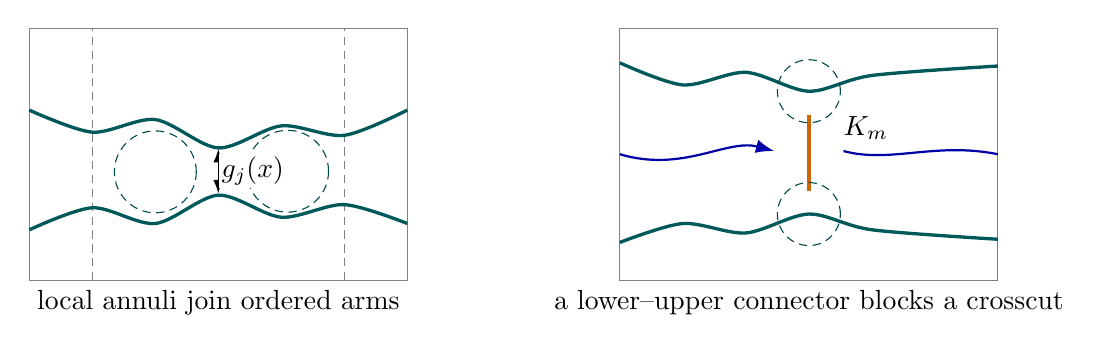
\begin{tikzpicture}[x=0.8cm,y=0.8cm,>=Latex]
 \draw[gray] (0,0) rectangle (6,4);
 \draw[densely dashed,gray] (1,0)--(1,4) (5,0)--(5,4);
 \draw[very thick,teal!70!black] plot[smooth] coordinates
   {(0,0.8) (1,1.15) (2,0.9) (3,1.35) (4,1.0) (5,1.2) (6,0.9)};
 \draw[very thick,teal!70!black] plot[smooth] coordinates
   {(0,2.7) (1,2.35) (2,2.55) (3,2.1) (4,2.45) (5,2.3) (6,2.7)};
 \draw[teal!60!black,densely dashed] (2,1.72) circle (0.65);
 \draw[teal!60!black,densely dashed] (4.1,1.73) circle (0.65);
 \draw[<->] (3,1.38)--node[right,fill=white,inner sep=1pt] {$g_j(x)$}
                  (3,2.08);
 \node at (3,-0.35) {local annuli join ordered arms};
 \begin{scope}[xshift=7.5cm]
  \draw[gray] (0,0) rectangle (6,4);
  \draw[very thick,teal!70!black] plot[smooth] coordinates
    {(0,0.6) (1,0.9) (2,0.75) (3,1.05) (4,0.8) (6,0.65)};
  \draw[very thick,teal!70!black] plot[smooth] coordinates
    {(0,3.45) (1,3.1) (2,3.3) (3,3.0) (4,3.25) (6,3.4)};
  \draw[very thick,orange!80!black] (3,1.42)--(3,2.63);
  \draw[teal!60!black,densely dashed] (3,1.05) circle (0.5);
  \draw[teal!60!black,densely dashed] (3,3.0) circle (0.5);
  \draw[blue!65!black,thick,->] (0,2.0).. controls (1.0,1.7) and
    (1.7,2.25)..(2.45,2.05);
  \draw[blue!65!black,thick] (3.55,2.05).. controls (4.3,1.85) and
    (5,2.2)..(6,2.0);
  \node[anchor=south west,inner sep=1pt] at (3.5,2.18) {$K_m$};
  \node at (3,-0.35) {a lower--upper connector blocks a crosscut};
 \end{scope}
\end{tikzpicture}
\caption{The two geometric steps in collar exclusion, drawn
schematically. Representative arms can double back; their topmost
vertical encounters remain ordered. The dashed matching circuits are
local geometric circuits, with any artificial part contained in the
forbidden cell region. In the right panel the compact gap segment
$K_m$ is forbidden to a sufficiently thin collar.}
\label{fig:spatial-collar}
\end{figure}

We finish by a compactness argument, keeping its choices deterministic.
If \eqref{eq:spatial-collar-limit} failed, there would be deterministic
allowed histories and walls at meshes $\delta_n\downarrow0$, widths
$\eta_n\downarrow0$, and a fixed positive lower bound for the traversal
probability. First fix $u$ so that \eqref{eq:spatial-gap-union}, summed
over the sides, is less than one quarter of that bound. One of the
finitely many surviving rank choices then has a fixed positive event
mass along a subsequence. We do not condition the law on that event.
Take Hausdorff limits, in the central buffered rectangle, of the
unions assigned below and above, including the virtual barriers.

Suppose first that the two limits touch there. Unless a virtual
barrier is involved, there are deterministic points on two
oppositely assigned pieces at distance $r_n\downarrow0$. Anchoring
makes both pieces cross the annuli from scale $r_n+O(\delta_n)$ to
a fixed outer scale. Any augmented matching circuit in such an
annulus joins them. By \eqref{eq:spatial-attached-arm}, the probability
of a traversal with this assignment tends to zero. If one limiting
piece is a virtual barrier, the fixed traversal margin rules out
the opposite assignment: a connected piece reaching that margin
lies on the barrier's side of the proper crosscut.

It remains that the two closed limits are disjoint in the central
rectangle. On a central vertical line choose a consecutive lower
encounter $a$ and upper encounter $b$. Such a transition exists
because the virtual bottom and top have those assignments. The open
segment $(a,b)$ misses both limiting unions. Fix an integer $m$.
At each actual endpoint choose $m$ separated circuit radii, all less
than $|a-b|/8$ and the available buffer clearance; call their smallest
radius $r_m>0$. If both endpoints are virtual, take any fixed
sufficiently small $r_m$ in their traversal margins instead.
Only after this choice, trim the gap by less than $r_m/2$ at its
ends and call the remaining compact segment $K_m$.
It has positive distance from the whole limiting obstacle union, not
just from its intersections with the vertical. This clearance holds
for the discrete obstacles for all large $n$, and then
$K_m\cap F_{\delta_n}^{\eta_n}=\varnothing$.

Center the endpoint tests at discrete points converging to $a$ and
$b$. An attached circuit at any of the chosen radii meets $K_m$:
it surrounds its center, and the ray into the gap crosses the circuit
between that radius and twice that radius. Its other intersection is
with the endpoint's anchored piece. For a virtual endpoint the short
segment in the fixed traversal margin supplies the connection instead.
Consequently a successful endpoint circuit at each actual endpoint,
together with $K_m$, is a connected set from a lower-assigned piece
or barrier to an upper-assigned one, wholly in the rectangle. Every
proper left-to-right crosscut with that assignment meets this set.
It cannot do so: it avoids the pieces and the attached circuits, and
the collar condition excludes $K_m$.

For fixed $m$, the probability that either required endpoint
connection fails has limit superior at most
$2C_k(1-p)^m$, by the separated-scale estimate and, if needed, one
density comparison. Letting $m$ increase contradicts the retained
positive event mass. The order of choices here matters: the finite
endpoint radii precede the trimmed segment, so every requested
circuit really reaches that segment. This proves uniformity in
\eqref{eq:spatial-collar-limit}.

Finally let a closed disk be bounded by an actual $W^{-\sigma}$ loop
and disjoint from $F_\delta$. A connected augmented matching circuit
attached to $F_\delta$ cannot enter this disk. Its artificial edges
are in $F_\delta$, outside the disk, and its actual $W^\sigma$ edges
cannot cross or share a vertex with the opposite-color boundary.
A dual path inside the disk therefore automatically avoids all those
circuits. The existence event already ranges over every underlying
dual path, so the bound holds simultaneously over the possible disks,
without conditioning on a future choice of one. Choosing all the
windows with fixed margin inside an open band gives the last
localization assertion. Monotonicity in $\eta$ gives the conclusion
for $\eta_\delta\downarrow0$.
\end{proof}

\subsection{Counts and comparison of complete patterns}

\begin{proposition}[Cluster and transmission counts]
\label{prop:cluster-counts}
The following bounds hold in fixed buffered boxes, uniformly in the
mesh and in allowed conditional histories. A joint count of actual
clusters across chambers in items~1 and~3 requires the product class
with a common fill. Item~2 has the interior scope stated there.
\begin{enumerate}
\item For fixed $b>0$, the number of unsearched free $N$ clusters
having a connected passage of diameter at least $b$ in a fixed box
has an exponential tail. Its constants depend on $b$ and the fixed
box geometry, not on the roughness of the surrounding walls or on
the number of chambers in the realization with a common fill.
\item For one chamber, let a rectangle and its joining buffer lie
wholly in the unprescribed accessible interior. Use the relative dual
restriction with separate side ports defined in the proof. The number of distinct
components of the restricted $N$ graph crossing between two specified
opposite sides has a geometric tail. Consequently, if
$Q_0\Subset Q_1$, the number of restricted components in $Q_1$
which meet $Q_0$ and a vertex incident to an edge outside the
restriction has a geometric tail, provided the fixed covering
rectangles in $Q_1\setminus Q_0$ and every joining buffer have the
same unprescribed interior clearance. Arbitrary admissible $(s,W)$
prescriptions outside a larger buffer are allowed. The same interior
assertion holds in the original wired law before removal of its
boundary cluster.
\item Counts of distinct free $N$ clusters of the residual kernels
enclosing or passing through a fixed
aspect-ratio annular shell have moments of every fixed order, uniformly
after rescaling the shell down to lattice order. Under a stopping
history these are the unsearched clusters. A distinguished wired
cluster adds at most one. For arbitrary
independent chambers with pairwise disjoint interiors this last
statement is available separately in each chamber; it asserts no
bound for their total count without a common fill. The precise
no-shadowing consequence at indexed discoveries is stated in
\cref{cor:indexed-no-shadowing} below.
\end{enumerate}
\end{proposition}

\begin{proof}
For item~1, start with the connected cell region of the given
exact cut history; for a single flat chamber use its exterior side.
Explore with a deterministic connected seed attached to that region.
Add one seed vertex at a time and immediately reveal the entire
previously undiscovered $N$ cluster it meets. The seed eventually
visits every vertex of the box. Record only discoveries with the
specified passage, choosing one such passage by a deterministic rule.
At every recorded stop, the initial region, seed, and all clusters
already discovered form one connected cell region. By
\cref{lem:finite-cuts}, the residual laws are exactly the flat
kernels, jointly in the class with a common fill when there are several
chambers.

A finite family of smaller collar windows detects every passage
of diameter at least $b$. Freeze the cell region $F_i$ at the
$i$th recorded stop, with $F_0$ the initial region, before continuing
the search. An actual unsearched $N$ path is disjoint from $F_i$ and
cannot cross the actual part of an augmented matching circuit.
Thus \cref{lem:collar} gives an $\eta>0$ such that, conditionally on
any such frozen history, the probability that \emph{some} still
unsearched qualifying passage lies wholly in $F_i^\eta$ is at most
a fixed $p<1$. This event is existential over future passages; no
future location or visibility is conditioned upon. It also bounds
the event that the next recorded cluster exists and its selected
passage lies wholly in $F_i^\eta$.

On the complementary event, the next passage contains a point at
distance greater than $\eta$ from $F_i$. Such points from successive
records are mutually $\eta$-separated, because each earlier cluster
is included in every later frozen region. A bounded box contains
at most $M=M(\eta)$ such points. There is no cost for the number
of intervening microscopic discoveries: they only enlarge the same
connected region. In the product case reflect the residual chamber
spins to one matching color and use the exact realization with a common fill
for this single existential collar event. In particular, no union
bound over the number of holes is taken. A test buffer meeting the
initial wall is covered by the same augmented graph.

If at least $n$ records occur, at most $M$ of the first $n$ can be
of the separated-point kind. Conditional iteration for the other
indices, including the initial stop, gives
\begin{equation}\label{eq:spatial-count-tail}
 \P[\text{at least }n\text{ recorded discoveries}]
       \le \sum_{j=0}^{M}\binom{n}{j}p^{\,n-j}
       \le C e^{-c n}.
\end{equation}
The same proof starting from a later allowed stop bounds its
unsearched count. It does not bound the number already fixed
by that history. Meshes above the small threshold used by the collar
lemma are absorbed by the deterministic number of vertices in the
fixed box.

For item~2 we adapt the crossing exploration underlying
\cite[Section~19.1, especially Lemmas~19.1 and~19.4]{DKLM2026}.
First fix the relative planar dual of the given restricted $N$
lattice quadrilateral. Its medial boundary follows the four sides
of the rectangle. In the auxiliary $W$ graph, truncate a dual edge
at that boundary when it exits, and give each boundary incidence
its own degree-one port. There are no edges in an exterior side
column and no identifications between distinct ports. Every retained
edge or half-edge inherits the state of its actual $W$ edge. This is the matched dual
restriction used for every $W$ connectivity test below; its
placement differs from the geometric rectangle by $O(\delta)$,
which is absorbed by the joining buffer.

If $J_N$ distinct restricted $N$ components cross the quadrilateral,
choose one simple crossing in each, ordered from bottom to top.
Between each two successive crossings, relative planar duality gives
a parallel open crossing of this matched $W$ graph. The separators
in two successive gaps belong to different components of that graph:
a connection inside it would cross the intervening $N$ path, and
the separate ports give no route around an endpoint. Consequently
\[
                  J_N\le J_W+1,
\]
where $J_W$ counts crossing components in precisely the matched
$W$ graph. The probabilistic search uses only these $W$ crossings;
it never certifies a separator against an unrevealed upper $N$ crossing.

Distinct $W$ crossing components have a consistent vertical order:
one component cannot have crossing paths on both sides of another,
because its joining path would cross the latter. In each component
choose a lowest simple proper crossing, with a deterministic tie
rule; the lower boundary of the union of its crossing paths supplies
such an open crossing. Enumerate these representatives from below,
with all connectivity restricted to the matched graph.
For a candidate $\gamma$, the event that it is the next distinct
crossing is determined by the $(s,W)$ configuration in its closed
below envelope. All lower candidate crossings lie there, and any
connection from a lower component to $\gamma$ first meets $\gamma$
from below. A proposed connection between lower pieces through the
region above $\gamma$ would first join $\gamma$ as well. This is
the stopping-line property for the enumeration.

After selecting $\gamma$, reveal the whole below envelope, with
endpoint spins before edge states. Calling the $W$ parity even,
extend endpoint half-edges only for the following geometric closure,
and close the envelope to an even domain $D_\gamma$ through the
unused side and bottom buffer outside the
central test balls. All earlier queried regions and their possibly
unfavorable frontiers are now inside $D_\gamma$; its boundary
segments in the central balls are exactly matching segments of
$\gamma$. The endpoint extensions are not edges of the counted
matched graph. The transcript is a cylinder measurable in $D_\gamma$.
Equivalently, one can disintegrate over that full cylinder after
the selection. The envelopes are nested as the search moves upward,
so the next transcript still has this form.

In a central vertical strip with a buffer continuing above the
rectangle, use the partial-circuit construction of
\cite[Lemma~19.4 and the proof of Lemma~19.1]{DKLM2026}. That lemma
is stated for the plane: it allows arbitrary same-parity data in
revealed even domains whose in-ball frontier is matching, and tests
a circuit in the matching graph augmented by those domains.
To transfer its bound to a finite conditional kernel, choose a
complete deterministic outer circuit $\Gamma_{\rm out}$ of the $W$
lattice, with its incident edge layer inside the unused buffer and
outside the test ball. Let $G^\circ$ be the graph induced by the $W$
vertices strictly inside $\Gamma_{\rm out}$, and let $V_\partial$ be
its vertices adjacent to that circuit. Analytically disintegrate the
old conditional law over the spins at $V_\partial$ and a complete
exterior and interface realization, fixing all endpoint spins before
edge states. For each fixed contact-spin vector, the positive exterior
fibers give laws on $G^\circ$ with identical retained interior pins
and local edge factors; only the same-color
partition of $V_\partial$ induced from outside varies. The interface
factors are constants once these endpoint spins are fixed. Every
exterior connection reaches $G^\circ$ through $V_\partial$. This
includes inherited abstract wires, whose terminals are outside the
unprescribed buffer.

For a sought plus circuit, replace this exterior partition by one
class on all minus contacts and singleton exterior classes on plus
contacts, retaining every interior pin and wire. This is the adverse
ordered boundary condition of \cref{prop:comparison}: it preserves or
merges every old minus connection and removes only plus exterior
connections. Realize it by pinning the vertices of $\Gamma_{\rm out}$
minus and its edges open. Pin each inward incidence $vc$, with
$v\in V_\partial$ and $c\in\Gamma_{\rm out}$, open minus if $s_v=-$
and closed if $s_v=+$; pin any interior chord of $\Gamma_{\rm out}$
open minus as well. These are compatible states after the endpoint
spins are fixed. An old minus-open incidence remains open, an old
plus-open incidence is closed, and an old closed incidence is either
kept closed or opened minus. The comparison is between kernels on
the common graph $G^\circ$; it does not impose the old exterior pins
on this new realization. Reflect colors for a sought minus circuit.

Under the complete cut $\Gamma_{\rm out}$, the finite interior
$(s,W)$ law and the plane law conditioned on the same cut have the
same flat kernel. Condition both on the identical retained interior
pins, contact spins, inward incidence states, and interior chords.
Cover the full added interface layer by finitely many small even
domains whose closures remain outside the test ball. Together with
$D_\gamma$, they make this conditioning measurable in the auxiliary
domain union, while adding no in-ball frontier segment or augmented
edge in the tested annulus. Lemma~19.4 applies in this plane
representation, with exactly the matching in-ball frontier of
$\gamma$, and gives the uniform positive partial-circuit bound.
The ordered comparison holds for every old fiber, so averaging with
its original probability introduces no factor. The original wired law
uses the same $(s,W)$ comparison before the cut. Multiple frontier
segments are handled by the finite-family conclusion of Lemma~19.4;
the polar Markov statement in Lemma~14.13 itself has only two arcs.

Intersect a fixed chain of these tests under the conditional pin
FKG law. With a fixed positive probability their augmented tube
joins the filled lower part to above the rectangle. It stays in
the central strip, where its last exit from $D_\gamma$ is on
$\gamma$ itself. The remaining connection is actual and lies in
the interior of the matched graph up to the top. A later parallel
crossing of the same color would meet it and join $\gamma$ within
that graph, while a crossing of the opposite color cannot cross it.
Thus the tube event rules out another distinct $W$ crossing.

These tube tests are used to bound the conditional probability;
their upper data are not added to the next search transcript.
For every transcript at the $i$th representative,
the conditional chance of a further one is at most $1-p$.
Iteration gives a geometric tail for $J_W$ and hence for $J_N$.
Connections outside the rectangle play no role because both counts
use restricted components. The original wired law has the same
interior $(s,W)$ comparison by \cref{prop:circuits}.

A fixed finite rectangle cover of the shell between $Q_0$ and $Q_1$
assigns each transmitting restricted component to a crossing of one
of these rectangles. The small lattice layer in the incidence
definition is absorbed by the fixed clearance. This proves the
transmission assertion.

For the shell assertion, the clusters counted are unsearched global
free clusters of the residual law, rather than distinct restricted
components. At shell
radius $r$, a fixed finite cover assigns every enclosing or passing
cluster a connected passage of diameter at least $c_2r$ in one
of its boxes. Apply item~1 after rescaling by $r$. Its collar proof
is uniform when $\delta/r$ is small, including boxes met by matching
walls in the realization with a common fill. When $\delta/r$ is bounded
below there are only a bounded number of vertices in the rescaled
boxes. The resulting exponential tail gives every fixed moment,
uniformly down to lattice order. For disjoint independent chambers
apply this assertion separately in each one. A pair of vertices in
different chambers shares no cluster, which is the only
cross-chamber fact needed for the later moment estimates.
\end{proof}

\begin{corollary}[Counts in an enclosing box]
\label{cor:global-cluster-counts}
Fix a bounded box $L$ and $b>0$. Suppose the finite lattice domain
and the supports under consideration lie in $L$, and place $L$ in
a fixed larger regular ambient box. For one free flat $N$ law, or
the residual product law with a common fill conditional on its initial
exact cut data, let
\[
 \mathcal N_\delta(b)
   =\#\{\,\text{free }N\text{ clusters }C:\diam C\ge b\,\}.
\]
There are constants $C,c>0$, depending on $L,b,t$ but not on the
initial walls or the mesh, such that
\begin{equation}\label{eq:spatial-global-count-tail}
       \P[\mathcal N_\delta(b)\ge n\mid\text{initial cut data}]
                       \le C e^{-cn}.
\end{equation}
The unconditioned free dual current is included. For the original
wired current, expose its boundary cluster first; its free
descendants satisfy this estimate conditionally, and adding the
distinguished boundary cluster increases the count by at most one.
The boxes and all cover buffers are fixed before the mesh limit.

There is also a pathwise consequence for a seed exploration. Suppose
a compact set $Q$ is at distance at least $r>0$ from the seed and
initial removed support. List the discovered free clusters whose
support meets $Q$, or whose union of odd holes meets $Q$. If
$\mathcal L_\delta(\tau;Q,r)$ is the number listed up to any stop,
then, for all sufficiently small $\delta$,
\begin{equation}\label{eq:spatial-contributor-domination}
       \mathcal L_\delta(\tau;Q,r)
                       \le \mathcal N_{\delta,\mathrm{initial}}(r/3).
\end{equation}
Add one on the right if the distinguished wired cluster is listed.
This is domination by the initial count, not a tail conditional on
the completed stop.
\end{corollary}

\begin{proof}
Cover $L$ by finitely many inner squares of side a small fixed
multiple of $b$. Around each choose a passage square and a larger
buffer, with fixed ratios, in the regular ambient box. If a
connected cluster has diameter at least $b$, choose two of its
points at that separation and an inner square containing the first.
The path to the second has a first exit from the passage square;
its initial portion is a connected passage of diameter at least
$c_1b$ there, for a fixed $c_1>0$. Let
$\mathcal N_{\delta,i}^{\rm passage}(c_1b)$ be the item~1 count
of unsearched global free clusters of the initial residual law
having such a passage in the $i$th square.
Every global cluster is counted in at least one of these counts.
Consequently
\[
        \mathcal N_\delta(b)
            \le \sum_{\text{cover squares }i}
                 \mathcal N_{\delta,i}^{\rm passage}(c_1b).
\]
The cover is fixed before $\delta$. Its passage buffers may cross
the original boundary or the revealed wired layer: extend the
initial cell region to the ambient box and use the augmented
matching completion of \cref{prop:circuits}. Item~1 of
\cref{prop:cluster-counts} and a finite union bound give
\eqref{eq:spatial-global-count-tail}. For the original free dual
law the matching primal boundary is the initial fill. Behind the
wired $N$ boundary cluster, \cref{lem:finite-cuts} gives precisely
the product law whose common initial fill is that connected cluster
joined to the exterior.

For \eqref{eq:spatial-contributor-domination}, every discovered
cluster meets the seed. If its support meets $Q$, it has diameter
at least $r-O(\delta)$. If instead one of its odd holes meets $Q$,
that hole lies in the convex hull of the cluster's cell region:
a bounded complementary component is contained in that convex
hull. A point of the hole is therefore at distance at most
$\diam C+O(\delta)$ from the seed contact on $C$. This again gives
$\diam C\ge r-O(\delta)$. The listed clusters are distinct members
of the initial free collection, proving the pathwise inequality.
This argument covers a cluster which surrounds $Q$ without meeting it.
\end{proof}

\begin{lemma}[Distance to a chamber-side rim]\label{lem:chamber-rim-distance}
Let $U_\delta$ be a resolved residual chamber of an exact cut
exploration, let $S_\delta$ be the revealed support including the
initial boundary and seed as needed, and let $\Gamma_\delta$ be its
own chamber-side
$W$ perimeter. For any subset $C_\delta$ of that chamber,
\begin{equation}\label{eq:spatial-own-rim-distance}
 \sup_{x\in C_\delta}\dist(x,\Gamma_\delta)
       \le \sup_{x\in C_\delta}\dist(x,S_\delta)+O(\delta).
\end{equation}
The constant is the lattice resolution constant. In particular, if
$C_\delta\to C_*$ and $S_\delta\to S_*$ in Hausdorff distance with
$C_*\subset S_*$, the left side tends to zero.
\end{lemma}

\begin{proof}
For $x\in U_\delta$, take a segment to a nearest point of
$S_\delta$. Its first exit from the resolved chamber meets that
chamber's own medial perimeter, within $O(\delta)$ of the
corresponding $W$ edge. The distance to this first exit is at most
the length of the segment. Taking suprema proves the inequality.
This uses the own perimeter even if the nearest support point
belongs to another nearby part of a pinched wired layer. For the
original free chamber the same argument uses its polygonal boundary
as $S_\delta$. The Hausdorff conclusion follows from the one-sided
inclusion $C_*\subset S_*$.
\end{proof}

\begin{corollary}[No shadowing at recorded stops]
\label{cor:indexed-no-shadowing}
Fix a buffered box $Q$ and $b>0$. At a stop $\tau$ of an
exterior-attached seed exploration, let $F_\tau$ be its frozen
connected cell region, including the initial walls, all visited seed
vertices, and all clusters already revealed. Let
\[
 \Xi_\delta(\tau;b,\eta)
  =\left\{\begin{array}{c}
   \text{some unsearched }N\text{ cluster has a connected}\\[-2pt]
   \text{passage }\gamma\subset Q,\quad \diam\gamma\ge b,\quad
              \gamma\subset F_\tau^\eta
          \end{array}\right\}.
\]
For allowed exact cut or $(s,W)$ stopping histories $\mathcal H_\tau$
with the supported residual product class,
\begin{equation}\label{eq:spatial-frozen-shadow}
 \P[\Xi_\delta(\tau;b,\eta)\mid\mathcal H_\tau]
       \le\omega_{Q,b}(\eta,\delta),\qquad
 \lim_{\eta\downarrow0}\limsup_{\delta\downarrow0}
       \omega_{Q,b}(\eta,\delta)=0,
\end{equation}
uniformly over positive probability histories. Exterior colors
rendered irrelevant by a completed cut are allowed. Arbitrary
interior $d$ pins, or conditioning on a later visibility event,
are not part of this statement.

For an exploration in the enclosing box of
\cref{cor:global-cluster-counts}, index stops by their rank among
discoveries of clusters of diameter at least $b$, and let
$\tau_0$ be the initial stop. All intervening smaller discoveries
are included in each frozen $F_{\tau_i}$. If $D_\delta(b)$ is the
number of these records, then, for every integer $K$,
\begin{equation}\label{eq:spatial-indexed-shadow}
 \P[\exists\,0\le i\le D_\delta(b):
             \Xi_\delta(\tau_i;b,\eta)
       \mid\text{initial cut data}]
 \le C e^{-cK}+(K+1)\omega_{Q,b}(\eta,\delta).
\end{equation}
The indices here are recorded macroscopic ranks, not raw discovery
numbers.

If a random width $\eta_\delta$ tends to zero only on a limiting
event $E$, the usable deterministic inclusion is, for fixed $\eta$,
\begin{equation}\label{eq:spatial-random-width}
 E\cap\Xi_\delta(\tau;b,\eta_\delta)
 \subseteq
 \Xi_\delta(\tau;b,\eta)\ \cup\
       \bigl(E\cap\{\eta_\delta>\eta\}\bigr).
\end{equation}
Thus one first fixes $\eta$, takes the mesh limit (and Fatou's
inequality when passing to a limit event), and then sends $\eta$ to
zero. No estimate is asserted after conditioning on $E$.
\end{corollary}

\begin{proof}
An actual unsearched $N$ passage avoids $F_\tau$ and the actual
edges of every attached augmented matching circuit. A finite
collar-window cover of $Q$ therefore gives
\eqref{eq:spatial-frozen-shadow} from \cref{lem:collar}, including
windows met by the initial wall. The exact cut factorization
identifies the residual marginal for every permitted history.
The bound is for the existential future event under that marginal;
it does not reveal a particular future passage.

On $D_\delta(b)\le K$, there are at most $K+1$ frozen indexed
stops. Apply \eqref{eq:spatial-frozen-shadow} at each one and use
a union bound. The complementary event is bounded by
\eqref{eq:spatial-global-count-tail}, which yields
\eqref{eq:spatial-indexed-shadow}. Finally,
\eqref{eq:spatial-random-width} follows from monotonicity of
neighborhoods. It gives the stated order of limits even when the
width was chosen from a future Hausdorff containment.
\end{proof}

For subsequent analytic arguments an additive mixing estimate is
not sufficient: the prescribed microscopic patterns may themselves
have very small probability. We therefore record a multiplicative
comparison. A \emph{complete pattern} in a finite vertex-and-edge
set specifies all its $s$ spins and all its $W$ edge states. Every
specified edge includes its endpoints.

\begin{proposition}[Pattern comparison]
\label{prop:pattern-comparison}
Fix regular compact sets $Q_i$ and filled buffered neighborhoods
$B_i$, $1\le i\le m$, with the $B_i$ pairwise disjoint and a fixed
positive separation between $Q_i$ and $\partial B_i$. Assume each
$B_i$ is contained in the domain, with no prescribed data there
other than the pattern being tested in $Q_i$. Exterior data may be
arbitrary admissible $(s,W)$ data and their retained connections.
There is a constant $C$ such that, for complete patterns $p_i$,
\begin{equation}\label{eq:spatial-product-patterns}
 C^{-m}\prod_{i=1}^m\pi_i(p_i)
 \le \mu[p_i\text{ on every }Q_i]
 \le C^m\prod_{i=1}^m\pi_i(p_i).
\end{equation}
Here $\mu$ is any such conditional flat law, and $\pi_i$ is the
plane pattern law in $Q_i$. The constant depends on the fixed
buffer geometry and $t$, not on the patterns or on their number
of microscopic prescriptions. Copies under parity-preserving lattice
translations and reflections satisfy the same assertion.

In particular, the single-box pattern laws have uniformly bounded
Radon--Nikodym density ratios, and the same remains true locally
after conditioning on any collection of separated patterns in the
other boxes.
\end{proposition}

\begin{proof}
Consider first a single $Q$ inside its buffer $B$. Prescribe a
complete admissible pattern in four batches: its plus vertices,
its minus vertices, its increasing compatible edge prescriptions,
and its decreasing compatible edge prescriptions. After the first
two batches every edge endpoint is fixed. A disagreeing edge is
already determined closed. On monochromatic edges the two remaining
batches mean open plus or closed minus, and closed plus or open
minus, respectively. Each batch is monotone in one of the two
orders of \cref{prop:comparison}. The number of batches is four,
independently of the pattern size.

Fix the preceding batches and consider an increasing current batch
$E$. Choose two deterministic annular buffers between $Q$ and
$\partial B$, and fix a plus circuit on the farther one. Let $\lambda$
be the law inside that deterministic circuit with the preceding
prescriptions retained. Comparison gives
\begin{equation}\label{eq:spatial-batch-upper}
                         \mu(E)\le\lambda(E).
\end{equation}
In the nearer annulus, conditional on the preceding prescriptions,
a random plus circuit has probability at least $p>0$. To see this
even if those prescriptions contain both signs, cover that annulus
by buffered test boxes missing $Q$; the exterior bound for one parity
and FKG supply its circuit with the same positive constant.
Search outside-in, inspecting nothing on the sealed side, and stop
at the first such circuit in a fixed exploration. Its interior
law is plus wired by \cref{lem:finite-cuts}, and hence dominates
the restriction of $\lambda$, with the same preceding prescriptions.
Consequently
\begin{equation}\label{eq:spatial-batch-lower}
                         \mu(E)\ge p\lambda(E).
\end{equation}
The decreasing batch uses minus circuits and the reversed order.

The law $\lambda$ is common to any two exterior conditions under
comparison. Applying \eqref{eq:spatial-batch-upper}--
\eqref{eq:spatial-batch-lower} to each of the four conditional batch
probabilities yields bounded ratios for the complete pattern
probabilities. Zero-probability patterns are exactly the common
local incompatibilities and are harmless. These constants remain
valid when the comparison law is a flat exhaustion of the plane.
The common plane spin/percolation law obtained from flat exhaustions in
\cite[Theorem~17.1]{DKLM2026} therefore gives the comparison with
$\pi_i$ by taking that exhaustion limit. For fixed $W$ parity this
law is invariant under parity-preserving lattice translations and
reflections, with the compatible global residue action. An
automorphism exchanging the lattices acts also by exchanging which
parity is called $W$; it is not invariance of the same fixed edge
decoration under that automorphism. The height-gradient marginal
has the full corner-grid symmetries used later.

For several boxes, condition successively on the patterns in the
other boxes. These constraints lie outside the current filled
buffer, so the single-box estimate applies with unchanged constants.
The chain rule gives \eqref{eq:spatial-product-patterns}. Conditioning
on separated patterns and repeating the same argument proves the
last assertion. Notice that the proof is multiplicative at every
stage; it is not an inference about rare events from a total
variation error.
\end{proof}

\subsection{Extending separation witnesses}

The preceding proposition concerns one spin parity and its edge
decoration. The other spins color complementary components, so their
admissible assignments can depend on connections outside a tested
pattern. We now localize that dependence. In this subsection choose
$W$ on the parity carrying the flat wall. The complementary $N$
components in the chamber are all free. This restriction is needed
only for the color statement here and below; the wired bulk circuit
case of \cref{prop:circuits} remains available.

Fix regular boxes $Q\Subset Q'\Subset B$ with fixed positive gaps.
For a geometric closed set, its complete pattern includes every $W$
edge meeting the set and both endpoint spins; the resulting one-mesh
boundary layer is part of the pattern. Form the restricted $N$ graph
using precisely the dual edges whose $W$ states that pattern
determines. A restricted component is a \emph{terminal} if it meets
$Q$ and contains a vertex incident to an unprescribed $N$ edge.
Every component meeting $Q$ that is not a terminal is sealed by the
pattern, so its color is independent of the exterior. This incidence
definition avoids losing an edge in the lattice boundary layer.
Select one marked vertex of each terminal by a deterministic rule.
A vector of signs on these marks is \emph{compatible} with an
exterior configuration if no two oppositely assigned marks become
connected in the full $N$ graph.

\begin{lemma}[Buffered separation witnesses]
\label{lem:buffered-witnesses}
Fix $p>0$ and an integer $k$. Conditional on any complete pattern
in $Q'$ with at most $k$ terminals, suppose a specified terminal
assignment has compatibility probability at least $p$ in a
$W$-flat domain containing $B$. There is
$c=c(p,k,Q,Q',B,t)>0$ such that, for every sufficiently small mesh,
with conditional probability at least $c$, every opposite pair
of marks is separated by an actual open monochromatic $W$ loop
contained in $B$. Thus compatibility is witnessed without using
the configuration beyond $B$. The estimate is uniform in the
microscopic pattern and in the enclosing domain.

Admissible $(s,W)$ exterior data beyond a fixed larger buffer are
allowed. No transverse $d$ colors are conditioned upon in this
statement.
\end{lemma}

\begin{proof}
In a finite $W$-flat domain, planar cut-cycle duality says that two
marks disconnected in $N$ are separated by a simple monochromatic
$W$ loop, allowing portions of the matching outer perimeter. We
will replace possibly long loops by loops in successively enlarged
cores. Write $\mathcal O$ for the set of required opposite pairs
and $m=|\mathcal O|\le k(k-1)/2$. If $m=0$ there is nothing to prove.
Choose regular closed cores
\[
       Q'=K_0\Subset K_1\Subset\cdots\Subset K_m\Subset B.
\]
In each gap fix a middle annular band and a wider band compactly
inside the gap, with further positive margins. At lattice scale
the core includes every $W$ edge meeting the closed core and its
endpoints. This convention counts a crossing on its boundary; all
such edges of $K_m$ lie in $B$ for small mesh.

For a complete pattern $g$ on $K_j$, let $\mathcal S(g)\subseteq
\mathcal O$ be the pairs separated by some actual monochromatic
loop in that lattice core. This set is determined by $g$ and can
only increase when the core pattern is enlarged in the same
configuration. A pair outside $\mathcal S(g)$ is called missing.
We prove the following one-step statement. If, under the original
law conditional only on $g$, compatibility has probability at
least $a>0$ and some pair is missing, then
\begin{equation}\label{eq:spatial-witness-step}
 \P[\text{compatibility and }|\mathcal S(P_{j+1})|
             >|\mathcal S(g)|\mid P_j=g]\ge r(a,k)>0.
\end{equation}
The constants use the fixed bands of this step and are uniform in
$g$ and the mesh. Here $P_j$ denotes the complete core pattern.

First choose a finite type of witness configuration. On compatibility,
among simple loops separating a missing pair choose one whose enclosed
set $I$ of marks is inclusion-minimal, with a deterministic rule for
ties. It contains a nonempty proper subset of the marks. No missing
pair is wholly inside its disk. To prove this, let $C$ be the selected
loop and suppose a missing pair $a,b$ lies inside. Choose a witness
loop $D$ for that pair. If it meets $C$, their colors agree, since
opposite-color open $W$ paths cannot meet. Consider the finite planar
graph
\[
             H=(C\cup D)\cap\overline{\operatorname{int}C}.
\]
Every underlying dual path from $a$ to $b$ leaving
$\operatorname{int}C$ crosses $C$, and every such path staying
inside crosses $D$. Thus $H$ separates $a$ from $b$ in the full
plane. Planar cut-cycle duality extracts a simple cycle of $H$
separating them. Its disk lies in
$\overline{\operatorname{int}C}$ and contains one of $a,b$ but not
the other, so its marked set is a nonempty proper subset of $I$.
All its edges have the common color. If $C$ and $D$ are disjoint,
the disk of $D$ must lie inside that of $C$ and gives the same
contradiction. This proves the claim, including shared-edge and
tangency cases.

Call $C$ the target. For every missing pair wholly outside $I$,
choose a witness loop and record its color. Record also the target
color and $I$. Reflect the colors for the description so that the
target is plus. A chosen minus witness is disjoint from the target;
its disk is either disjoint from the target disk or contains that
disk. Of its two marked endpoints record the one on the side away
from the target disk. The whole type consists of these data,
including the ordered away-endpoint vector and the fixed mark
$i_0=\min I$. There are at most $L(k)<\infty$ types, independently
of the shapes of all loops. If the compatibility probability is at
least $a$, one type event $\mathcal T$ has probability at least
$a_0=a/L(k)$. Fix that type now. The sampling law remains the
original law conditional on $g$; it is not conditioned on
$\mathcal T$.

From its fixed away marks perform a deterministic exploration of
the full components of the underlying dual graph whose edges do
not cross an open $W^-$ edge. These are components of the
complement of $W^-$, not components of $N$. Explore through already
known core edges as well as new ones, revealing endpoint spins
before each new edge state, until each component is exhausted.
There are at most $k$ distinct source components. The transcript
$h$ is the cylinder of the queried values, so its residual law
$\mu_h$ is an allowed pin law in \cref{prop:comparison}. In
particular it remains positively associated. The interior frontier
of a full source component consists of actual $W^-$ edges; it is
not a frontier artificially stopped at the old core. Original
outer-boundary conditions are retained, and the middle-band test
windows are away from the old core and the outer boundary.

Let $F_h^0$ be the union of the source cell regions of these
full components, without filling any complementary pocket. On
$\mathcal T$, each chosen minus witness prevents the source on its
away side from reaching the target disk. Thus the entire $F_h^0$,
including its frontier, misses that disk. The transcript also
certifies the selected minus separations: the other endpoint of
each such pair is outside its explored complement-of-$W^-$
component. Every $N$ edge belongs to that complement graph, so these
certificates imply the corresponding $N$ disconnections. Denote them by
$\mathcal C(h)$.

In the residual law, let $\mathcal U_h$ be the event that there
exists an actual plus target loop enclosing exactly $I$, whose
closed disk misses $F_h^0$, together with actual plus witnesses
for the specified missing outside pairs of plus type. This event
is increasing in \eqref{eq:spatial-order}. The minimality rule and
the identities of the previously selected loops have been dropped;
they would not be increasing. If $\nu_g$ is the law of the
transcript under the original law conditioned on the core, the implication
from $\mathcal T$ gives
\[
 a_0\le\int \ind_{\mathcal C(h)}\,
                  \mu_h(\mathcal U_h)\,\nu_g(\dd h).
\]
It follows that the histories satisfying $\mathcal C(h)$ and
$\mu_h(\mathcal U_h)\ge a_0/2$ have $\nu_g$ mass at least $a_0/2$.
We work separately under each such $\mu_h$. There is no FKG or
circuit estimate under the mixture conditioned on this choice of
histories.

For this fixed history choose the accessible component $U_h$ of
the complement of the raw region $F_h^0$ containing the already
fixed mark $i_0$. Histories with $i_0\in F_h^0$ have
$\mu_h(\mathcal U_h)=0$ and do not occur in the retained family.
Every target disk in $\mathcal U_h$ is connected, contains $i_0$,
and misses $F_h^0$, so it lies in this one component $U_h$.
Only after choosing $U_h$, add the other complementary pockets
to the forbidden cell region and call the resulting region $F_h$.
This addition is for the marginal collar test alone. It does not
discard any actual residual variable from $\mu_h$; plus witnesses
for other pairs may still lie in those pockets.

For each individual connected source, the connected set $U_h$
lies in one component of its complement and hence faces one
incident boundary walk of that source. It may face that walk at
many entrances, but there are at most $k$ source labels in total.
Against $U_h$ the frontier is actual minus in the middle band.
The exact completion of one component of \cref{prop:circuits} therefore
applies there; any use of a partition comparison has the same
$k$ indivisible labels. The added pockets attach to these sources,
so every local piece in the band is anchored back to a source mark
in the old core or to the outer boundary. A target disk remains
disjoint from $F_h$.

Put $b_0=a_0/2$. Choose a collar width $\eta>0$, uniformly in the
retained histories, so that \cref{lem:collar} bounds by $b_0/2$
the existence of a full underlying dual traversal of the middle
band which lies in $F_h^\eta$ and avoids $F_h$ and its attached
minus circuits. Use the selected $U_h$ marginal for this estimate.
The full residual law $\mu_h$ is retained for all other events.
The virtual-disk clause makes this a simultaneous bound for
traversals inside any target disk in $\mathcal U_h$. In particular,
we subtract this error from $\mu_h(\mathcal U_h)$; we do not
condition the law on absence of the collar event.

We spell out the increasing event supplied by this subtraction.
Write $K$ for the enlarged lattice core, $A$ for its fixed middle
band, and $A^+$ for the wider band. Choose a fixed regular outer
dual graph $R$ inside $B$, containing $K$ with a complete connected
annular
shell outside $K$. In the path tests below every underlying dual
edge of $R$ is available, regardless of its $N$ state or whether
it crosses a minus edge or the forbidden region. For each required
pair across $I$, orient paths from its $I$ mark, and require every
simple underlying path $\gamma$ between the two marks to satisfy
\begin{equation}\label{eq:spatial-temporary-alternative}
 \begin{array}{c}
 \gamma\text{ crosses an actual }W^+\text{ edge in }K,\\
 \text{or}\\
 \gamma\text{ has a subpath }\beta\subset A
 \text{ from the inner to the outer boundary of }A\\
 \text{which visits a point }z\text{ with }\dist(z,F_h)>\eta .
 \end{array}
\end{equation}
Intersect this requirement with the actual plus separations for
the specified outside pairs, and call the event $\mathcal V_h$.
The path family is finite and fixed by $R$; $F_h$ is fixed by $h$.
Only the first alternative changes with $W^+$. Thus
$\mathcal V_h$ is increasing. Neither $F_h$ nor any minus edge is
a real barrier in this definition.

On $\mathcal U_h$ outside the collar event, \eqref{eq:spatial-temporary-alternative}
holds. Indeed a path avoiding the actual $W^+$ edges in $K$ must
exit $K$ before its first crossing of the target loop. An edge
meeting the closed core is counted in $K$, so a first crossing
on its boundary cannot be lost. The path prefix before that
target crossing lies in the target disk. Before its first exit
from $K$, take the segment from its last hit of the inner band
boundary to its first subsequent hit of the outer one. This is
a full subpath $\beta\subset A$, even if the original path made
earlier excursions. It lies in the target disk and therefore
avoids $F_h$ and all attached minus circuits. Absence of the
collar event forces it to visit a point at distance greater than
$\eta$. Hence
\begin{equation}\label{eq:spatial-temporary-probability}
                   \mu_h(\mathcal V_h)\ge b_0/2.
\end{equation}

We replace the second alternative by actual plus circuits. Choose
a deterministic grid in $A$ of mesh much smaller than $\eta$ and
than the separation of its two boundary curves. For each cell
whose filled buffer is disjoint from $F_h$ and contained in $A^+$,
request an actual plus circuit surrounding the cell in that buffer.
Choose the grid and buffers so that every point of $A$ at distance
greater than $\eta$ from $F_h$ lies in an inner cell surrounded by
one requested circuit, and the disk of every such circuit has diameter
smaller
than the distance between the two boundary curves of $A$. This
is possible by taking the cell size a sufficiently small fixed
multiple of $\eta$ and of the band width. There are at most
$M=M(\eta)$ cells. Their buffers miss all source queries and the
old core; for small mesh they exceed the lattice cutoff.

Under the full residual pin law $\mu_h$, each requested actual
plus circuit has probability at least $p_1>0$ by
\cref{prop:circuits}. Positive association intersects all these
increasing events with $\mathcal V_h$, giving probability at least
$(b_0/2)p_1^M$. On their intersection, no across-$I$ path can
avoid the actual plus edges in $K$. Otherwise
\eqref{eq:spatial-temporary-alternative} supplies a full band
subpath visiting the interior of one requested circuit. A connected
path avoiding that circuit and visiting its interior must stay
inside its disk. Its two band-boundary endpoints cannot both lie
there, by the diameter choice. This contradiction realizes the
temporary alternative using actual plus edges only.

For completeness, separation in the graph $R$ gives actual closed
witness loops in $K$. Any path using a more distant exterior can
have each exterior excursion replaced in the complete connected
shell of $R$ outside $K$. Thus separation in $R$ is separation in
the full underlying dual graph by $W^+\cap K$. Planar cut-cycle
duality yields a simple plus loop in $K$ for each across pair;
a boundary-to-boundary cut is impossible because these blocking
edges lie strictly inside $R$. Artificial fill and minus edges
play no role in this final separation.

The history certificates protect the outside minus pairs. The
outside plus pairs are protected by $\mathcal V_h$, the across
pairs by the new local plus loops, and there was no missing pair
wholly inside $I$. Previously short loops are fixed in $g$.
Therefore compatibility holds and at least one missing pair has
joined $\mathcal S(P_{j+1})$. The retained histories have
$\nu_g$ mass at least $b_0$, so the construction proves
\eqref{eq:spatial-witness-step} with, for example,
\[
             r(a,k)=\frac{b_0^2}{2}\,p_1^{M(\eta)}>0,
       \qquad b_0=\frac{a}{2L(k)}.
\]
The collar width, grid, and mesh threshold were chosen from
$a,k$ and the fixed bands, not from the particular core pattern.
Replace $r(a,k)$ by its minimum over the finitely many band groups.

We finally iterate without retaining the long source histories.
Let $\mu$ be the original law conditional on the initial pattern,
and set
\[
 \mathcal G_j=\{\text{compatibility and }|\mathcal S(P_j)|\ge j\}.
\]
Initially $\mu(\mathcal G_0)\ge p$. If
$\mu(\mathcal G_j)\ge q_j>0$, disintegrate \emph{this original law}
only by the complete pattern $P_j$. Patterns with
$|\mathcal S(P_j)|\ge j$ and posterior compatibility at least
$q_j/2$ have total mass at least $q_j/2$: the other patterns
contribute at most $q_j/2$ to $\mu(\mathcal G_j)$. If such a
pattern already has $j+1$ short pairs, its conditional contribution
is at least $q_j/2$; otherwise apply
\eqref{eq:spatial-witness-step}. Hence
\[
 \mu(\mathcal G_{j+1})\ge
       \frac{q_j}{2}\min\left\{\frac{q_j}{2},
                                  r(q_j/2,k)\right\}
             =:q_{j+1}>0.
\]
At the next step all source transcripts and selected type events
have been integrated out. The new conditional law is again the
original law given only its complete core pattern, so its unused
buffers have the pin/FKG law required above. After $m$ steps all
pairs have short witnesses in $K_m\Subset B$, with probability
at least $q_m$. All widths and the finitely many mesh thresholds
are chosen before taking the mesh limit. This proves the lemma.
\end{proof}

\begin{proposition}[Full-spin contiguity]
\label{prop:full-contiguity}
Fix compactly nested regular boxes $Q\Subset B$ in the interior
of a $W$-flat domain, with fixed positive buffer ratios. Thus the
complementary $N$ components are free. Let $\mu_\delta$
be its law and $\pi_\delta$ the plane law, restricted to the full
spin pair in $Q$. The domains and any allowed exterior $(s,W)$
data may depend on $\delta$, but their walls and prescriptions stay
outside $B$. There is a uniform contiguity modulus: for every
$\eps>0$ there is $\zeta>0$ such that, for every sufficiently small
mesh and every event $E$ determined by the full spin pair in $Q$,
\begin{equation}\label{eq:spatial-contiguity}
             \pi_\delta(E)<\zeta
           \quad\Longrightarrow\quad
             \mu_\delta(E)<\eps.
\end{equation}
The conclusion also holds if the tested data include $W$ in $Q$.
In particular it applies to mesh-dependent tests. Either flat
parity can be used by assigning $W$ to the parity carrying that
flat wall. This statement does not include a fixed-color wired
$N$ component before its removal.
\end{proposition}

\begin{proof}
Choose $Q\Subset Q'\Subset B'$ with
$B'\Subset B$, leaving the fixed buffers of
\cref{lem:buffered-witnesses}. Let $P$ be the complete $(s,W)$ pattern
in $Q'$, and let $T(P)$ be its number of terminals. By
\cref{prop:cluster-counts}, uniformly in both domain and plane laws,
\begin{equation}\label{eq:spatial-terminal-tail}
                       \P[T(P)>M]\le C e^{-cM}.
\end{equation}
Choose $M$ so that the right side is less than $\eps/4$ for the
domain law.

On $T(P)\le M$, write $b$ for an assignment of signs to its
terminals, and let $v_\mu(b\mid P)$ be its conditional exterior
compatibility probability. By \cref{lem:finite-cuts}, the actual
terminal-color probability $q_\mu(b\mid P)$ satisfies
\begin{equation}\label{eq:spatial-color-cost}
        2^{-M}v_\mu(b\mid P)
             \le q_\mu(b\mid P)\le v_\mu(b\mid P).
\end{equation}
Indeed, given a compatible exterior partition, specifying these
terminal signs costs $2^{-j}$ for some $j\le M$ distinct free global
components. The same calculation applies in the plane because
\cite[Theorem~17.1]{DKLM2026} gives no unbounded complementary
component and independent fair transverse colors. Components of
the restricted pattern not incident to an unprescribed edge carry
independent fair colors. Their distribution is the same under the
two laws once $P$ and the terminal signs are given. The lower
bound in \eqref{eq:spatial-color-cost} uses freeness; a terminal
wired to a prescribed incompatible color would not satisfy it.

Choose $p>0$ with $2^M p<\eps/4$. The total domain probability of
assignments with $v_\mu(b\mid P)<p$ is at most $2^M p$, by the
upper bound in \eqref{eq:spatial-color-cost}. For every remaining
assignment, \cref{lem:buffered-witnesses} gives short witnesses in
$B'$ with conditional probability at least $c(p,M)>0$.
Fix a realized pattern $g$ for $P$, and let $\mathcal W_b$ be this
short-witness event, determined by a
complete pattern in $B'$. If $C_{B'}$ and $C_{Q'}$ are the
unconditioned pattern density constants in
\cref{prop:pattern-comparison}, summing over the larger patterns
and then dividing gives
\[
 \pi_\delta(\mathcal W_b\mid P=g)
   =\frac{\pi_\delta(\mathcal W_b\cap\{P=g\})}{\pi_\delta(P=g)}
   \ge (C_{B'}C_{Q'})^{-1}
          \mu_\delta(\mathcal W_b\mid P=g).
\]
This uses only the original laws on one parity on the two pattern
sets, not a comparison after conditioning on $d$ or on the
witness event. Hence there is $c_0=c_0(p,M)>0$ such that
\begin{equation}\label{eq:spatial-plane-viability}
 v_\pi(b\mid P)\ge c_0,
 \qquad q_\pi(b\mid P)\ge 2^{-M}c_0
\end{equation}
whenever $v_\mu(b\mid P)\ge p$ and $T(P)\le M$.
There is no conditioning on $d$ in this comparison: the short
witness event concerns only $W$ and $s$.

Let $C_0$ be the uniform density-ratio constant for $P$ in
\cref{prop:pattern-comparison}. Conditional on $P$ and a terminal
assignment, integrate the identical independent internal colors.
On the retained assignments,
\eqref{eq:spatial-plane-viability} bounds the ratio of terminal-color
probabilities by $2^M/c_0$. Therefore every tested event satisfies
\begin{equation}\label{eq:spatial-contiguity-modulus}
       \mu_\delta(E)
       \le \frac{\eps}{2}
                + C_0\frac{2^M}{c_0}\,\pi_\delta(E).
\end{equation}
Choosing $\zeta<\eps c_0/(2C_0 2^M)$ proves
\eqref{eq:spatial-contiguity}. All constants were chosen from
$\eps$, the fixed geometry, and $t$ before the mesh limit, so the
modulus is uniform in the stated domain laws. Enlarging the tested
data by $W$ does not change the conditioning argument.
\end{proof}

The distinction between \cref{prop:pattern-comparison} and
\cref{prop:full-contiguity} is useful later. The former supplies
uniform multiplicative estimates even for extremely rare
patterns on one parity. The latter supplies domination in probability
for both spin parities, without asserting a bounded density ratio
for every possible microscopic color assignment.

\section{Reflection positivity and the plane covariance}
\label{sec:spectral}

This section identifies every subsequential plane covariance, without assuming
either Gaussianity or rotation invariance of a scaling limit. The positive
transfer method of \cite[Section~5]{Triangular} suggests the argument, but its
sixfold rotational cancellation is unavailable here. Two square-lattice
reflection frames at angle $\pi/4$ provide the required replacement.

We temporarily choose Euclidean units in which the corner grid is $\Z^2$.
This is a fixed rotation and dilation of the original embedding. The local
plaquette calculation above identifies its height weights with the
six-vertex weights $(1,1,c)$. The spin and decoration law obtained from flat
exhaustions is the measure of \cite[Theorem~17.1]{DKLM2026};
\cite[Lemma~18.7(iii)]{DKLM2026} identifies its height-gradient marginal
with the slope-zero six-vertex plane measure. By
\cite[Theorem~2.2]{DKLM2026}, that marginal is stationary under all
corner-grid translations and invariant under the lattice reflections.
The geometric height reflection used below sends $K$ to its composition
with the spatial reflection, up to an additive constant. In arrow variables
this combines spatial reflection with global arrow reversal; it also
preserves the finite plaquette weights directly.
These statements apply for every $1\le c\le2$. A uniform simultaneous
choice of the two spin signs is understood when residues rather than
increments are observed. In particular an odd corner-grid translation $T$
exchanges the parities with gauge
$(\tau',\tau^{\dagger\prime})=(\tau^\dagger\circ T,-\tau\circ T)$:
its height is $K'(x)=K(Tx)-K(T0)$. This preserves the incident-corner rule
and accounts for the change of reference parity.
The additive constant of $K$ is immaterial. For a smooth compactly supported
function $f$ of integral zero, use bilinear nodal interpolation on each
corner-grid square to define $K_\delta(f)$. This interpolation commutes with
all four row reflections and with grid translations.
Write its finite array of coefficients as $b_{\delta,x}$; their sum is
exactly zero. For a $2m$th moment, choose smooth mass-one reference
densities in $2m$ disjoint fixed disks outside the common support of the
tests. Let $r_{\delta,j,y}$ be nonnegative discretizations of these
densities, normalized so that $\sum_y r_{\delta,j,y}=1$. For each occurrence
$j$ the exact finite-sum identity is
\[
 K_\delta(f)
   =\sum_{x,y}b_{\delta,x}r_{\delta,j,y}\bigl(K(x)-K(y)\bigr).
\]
Use a separate reference index $j$ in each factor of the moment. The
regularity estimate \cite[Theorem~4.5]{DKLM2026} then applies to increment
correlations with separately summed reference variables. Its collision
singularities are products of logarithms, which are locally integrable;
the lattice cells of exact coincidence contribute at most a lattice area
times a fixed power of $1+|\log\delta|$. Integrating the estimate gives
\begin{equation}
 \sup_{0<\delta<\delta_0}\E|K_\delta(f)|^{2m}<\infty,
 \qquad m\in\N.
 \label{eq:plane-neutral-moments}
\end{equation}
The bounds are uniform for tests in a bounded smooth family with common
compact support. The estimate holds throughout $1\le c\le2$, not just the
range of the convergence theorem in that paper.
The elementary path-factor correction in its proof is supplied in
\cref{sec:input-path}.

\subsection{Four positive reflection frames}

\begin{lemma}[Positive normal transfer]
\label{lem:positive-transfer}
The plane law is reflection positive across a row of corner-grid sites in
each of the directions $0,\pi/4,\pi/2,3\pi/4$. In its reflection Hilbert
space, translation by two successive row spacings in the inward normal
direction is a positive self-adjoint contraction. For the height-increment
law, tangential translation by one row period is a commuting unitary.
Reflection positivity and positive normal transfer remain valid for local
spin and edge decorations strictly on one side of the row, and for
independent uniform phase lifts of the height. With a fixed one-parity edge
decoration, the tangential unitary assertion is restricted to
parity-preserving translations.
\end{lemma}

\begin{proof}
First use a finite reflection-symmetric flat exhaustion. Across an axial row,
plaquette interactions on the two sides factor after conditioning on the row
heights. Across a diagonal row, a straddling plaquette has the following
conditional weight matrix. If its two row heights are equal, the other
heights are independently one unit above or below that value. Equal
transverse heights have weight $c$, and unequal ones have weight one.
Consequently the matrix, after multiplication by $t$, is
\[
 \begin{pmatrix}1&t\\t&1\end{pmatrix}.
\]
It is positive semidefinite because $0<t\le1$. If the row heights differ
by two, the transverse heights are forced and there is only a scalar factor.
Factoring each positive matrix as a Gram matrix proves positivity after
summing the row data. Independent local decorations are included in the
factors on their own sides. Spin residues are determined by heights and one
compatible global sign choice, which can be fixed at an anchor on the row.
For a phase $U\exp(i\alpha(K(x)-K(o)))$, also condition on its value at that
anchor; $U$ has independent uniform law. Thus these augmentations preserve
the same Gram representation. Circuit comparison passes each reflected
exhaustion to the same plane law.

Let $\Theta$ be reflection in the row and set
$\langle F,G\rangle=\E[\overline{\Theta F}G]$ for functions on its inward
half-plane. Denote the pure normal translation through two row spacings by
$T$. Stationarity gives symmetry of $T$ for this form. Reflection positivity
at the intermediate row gives $\langle F,TF\rangle\ge0$. To prove boundedness
before quotienting, put $b_j=\|T^jF\|$. Reflection Cauchy--Schwarz gives
$b_j^2\le b_{j-1}b_{j+1}$, whereas ordinary Cauchy--Schwarz and stationarity
give $b_j\le\|F\|_{L^2}$ for all $j$. A bounded nonnegative log-convex
sequence cannot increase at its first step. Hence $\|TF\|\le\|F\|$, also
when $\|F\|=0$. Thus $T$ descends to a positive self-adjoint contraction.
Tangential translation preserves the form, has a form-preserving inverse,
and commutes with $T$, whenever it preserves the chosen state space. For
the height-increment law this includes one row period. With a fixed
one-parity decoration it includes two axial periods or one diagonal period;
the normal transfers used above already preserve that parity.
\end{proof}

In a frame with unit tangent $u$ and normal $v$, write the rectangular
sublattice just obtained as
\[
 \Lambda_0=\ell\Z u+d\Z v.
\]
For an axial frame one may take $(\ell,d)=(1,2)$; for a diagonal frame take
$(\ell,d)=(\sqrt2,\sqrt2)$. Each has finite index in the corner grid. All
frequency coordinates below are Euclidean: $p=ku+lv$. In particular, the
normal spectral scale and $|k|$ have the same physical units.
The spectral argument uses the undecorated height-increment space; the
decorated argument in \cref{sec:screening} uses only normal transfers.

\subsection{The spectral measure and its Cauchy disintegration}

\begin{lemma}[Increment spectral measure]
\label{lem:increment-spectral}
There is a nonnegative measure $C$, locally finite on the punctured reciprocal
torus of the corner grid, such that every finitely supported real array of
zero sum satisfies
\begin{equation}
 \E\left(\sum_x b_xK(x)\right)^2
   =\int\left|\sum_x b_x e^{ip\cdot x}\right|^2 C(\dd p).
 \label{eq:increment-spectral}
\end{equation}
There is no additional random linear tilt. For sufficiently small $r$,
\begin{equation}
 C\{r\le|p|\le2r\}\le C_0.
 \label{eq:spectral-annulus}
\end{equation}
Consequently $\int_{0<|p|<r_0}|p|^\eta C(\dd p)<\infty$ for every $\eta>0$.
\end{lemma}

\begin{proof}
Let $V_x$ be ordinary translation on the plane probability space, $E(\dd p)$
its spectral resolution \cite[Theorem~5.6]{WilliamsSpectral2018},
and $\xi_x=K(x)-K(0)$. The cocycle identity gives
\[
 (V_y-I)\xi_x=(V_x-I)\xi_y.
\]
On any spectral neighborhood where $e^{ip\cdot y}-1\ne0$, define
\[
 C(\dd p)=
 \frac{\langle\xi_y,E(\dd p)\xi_y\rangle_{L^2}}
 {|e^{ip\cdot y}-1|^2}.
\]
The identity makes the definitions agree on overlaps; two grid directions
cover the punctured torus. The invariant part is additive and has the form
$A\cdot x$ for a random vector $A\in L^2$. Smearing at scale $L$ against a
neutral test of first moment $m$ gives invariant part $LA\cdot m$.
Its norm is uniformly bounded by \cref{eq:plane-neutral-moments}, since
orthogonal projection cannot increase norm. Two independent choices of $m$
give $A=0$.

Choose two real neutral smooth tests whose Fourier transforms have no common
zero on $1\le|p|\le2$; derivatives in the two coordinate directions of a
sufficiently narrow smooth bump suffice. Their scale-$r^{-1}$ interpolation
transforms converge uniformly on this annulus to those transforms. The sum
of their squared absolute values is therefore bounded below on
$r\le|p|\le2r$. Apply \cref{eq:increment-spectral} and the uniform second
moment bound. Summing over dyadic annuli proves the last assertion.
\end{proof}

Project $C$ to the reciprocal rectangle
$[-\pi/\ell,\pi/\ell)\times[-\pi/d,\pi/d)$ of $\Lambda_0$, and call the
result $C'$. Besides the physical origin, the preimages of its origin are
finitely many nonzero reciprocal points, called aliases. Their neighborhoods
have finite mass; atoms at aliases are allowed.
Put $P=2\pi/d$. For $0<s<\infty$, define the probability law
\[
 Q_s(\dd l)=\sum_{j\in\Z}
 \frac{s\,\dd l}{\pi(s^2+(l+jP)^2)},\qquad -P/2\le l<P/2,
\]
with $Q_0=\delta_0$ and $Q_\infty$ uniform on the circle.

\begin{lemma}[Positive Cauchy mixture]
\label{lem:cauchy-mixture}
For $k\ne0$ there is a nonnegative mixing measure $\nu$ such that
\begin{equation}
 C'(\dd k,\dd l)=\int_{[0,\infty]}Q_s(\dd l)\,\nu(\dd k,\dd s).
 \label{eq:cauchy-mixture}
\end{equation}
It is finite on horizontal bands away from zero and satisfies
\begin{equation}
 \int_{0<|k|<\kappa}|k|\,\nu(\dd k,\dd s)<\infty
 \label{eq:weighted-mixture}
\end{equation}
for small fixed $\kappa$.
\end{lemma}

\begin{proof}
The row increment $F=K(\ell u)-K(0)$ belongs to the reflection Hilbert space.
The joint spectral theorem for its commuting tangential unitary and positive
normal contraction \cite[Theorem~5.6]{WilliamsSpectral2018} gives,
for $j\ge0$,
\[
 \E[F V_{n\ell u+jdv}F]
   =\int e^{in\ell k}\lambda^j\,\gamma(\dd k,\dd\lambda),
 \qquad 0\le\lambda\le1.
\]
Reflection gives the same expression with $|j|$. Set $\lambda=e^{-ds}$,
including $s=\infty$ when $\lambda=0$. These are precisely the vertical
Fourier coefficients of $Q_s$. Uniqueness of Fourier coefficients for finite
measures identifies the ordinary increment measure as this mixture. That
measure is $|e^{i\ell k}-1|^2C'$. Division for $k\ne0$ proves the formula.
Since every $Q_s$ has mass one, the integral in
\cref{eq:weighted-mixture} equals $\int|k|C'(\dd k,\dd l)$ over the same
band. Near the physical origin it is finite by
\cref{eq:spectral-annulus}; all other contributions have finite mass.
\end{proof}

\subsection{An angular defect in two frames}

Define
\[
 \chi(k,l)=\cos(4\arg(k+il))
       =1-\frac{8k^2l^2}{(k^2+l^2)^2},\qquad
 D(k,s)=\left(\frac{|k|-s}{|k|+s}\right)^2,
\]
where $D(k,\infty)=1$. Uniformly in $s\in[0,\infty]$,
\begin{equation}
 \int\chi(k,l)Q_s(\dd l)=D(k,s)+O(|k|),\qquad k\longrightarrow0.
 \label{eq:angular-poisson}
\end{equation}
For completeness, with $b=|k|$, the bounded analytic function
$((b+iz)/(b-iz))^2$ on the upper half-plane has boundary real part
$\chi(b,l)$. Its Poisson average at $is$ is $((b-s)/(b+s))^2$.
To periodize, use
\[
 1-\chi(b,l)=\frac{8b^2l^2}{(b^2+l^2)^2},\qquad
 \int_\R(1-\chi(b,l))\,\dd l=4\pi b.
\]
The sum of noncentral Cauchy densities over one period is uniformly bounded
in $s$. Indeed split its sum at $|j|$ comparable to $s/P$ and use $1/s$
for the nearer terms and a summable square tail for the rest. The omitted
unfolded tail of $1-\chi$ is $O(b^2)$. This proves
\cref{eq:angular-poisson}, including its two limiting laws.

\begin{proposition}[Summable dispersion defect]
\label{prop:dispersion-defect}
In each of the four reflection frames,
\begin{equation}
 \int_{0<|k|<\kappa}D(k,s)\,\nu(\dd k,\dd s)<\infty,
 \qquad
 \nu\{r\le|k|\le2r\}\le C_1.
 \label{eq:dispersion-defect}
\end{equation}
The second bound holds for every $r>0$.
\end{proposition}

\begin{proof}
Integrate \cref{eq:angular-poisson} over $\eps<|k|<\kappa$.
Its error is bounded independently of $\eps$ by
\cref{eq:weighted-mixture}. Replacing $C'$ outside the small physical disk
by the original measure costs bounded outer and alias mass. In the radial
annulus $\eps<|p|<\kappa$, the omitted endcap $|k|\le\eps$ has negative
fourth harmonic only where $|p|\le C\eps$: negativity implies
$|l/k|<1+\sqrt2$. Its negative part is bounded by a fixed number of the
annuli in \cref{eq:spectral-annulus}. Thus, in a frame of angle $\theta$,
\begin{equation}
 \int_{\eps<|k|<\kappa}D\,\dd\nu
 \le \int_{\eps<|p|<\kappa}
        \cos(4(\arg p-\theta))\,C(\dd p)+C_2.
 \label{eq:frame-defect-bound}
\end{equation}
Choose the same physical inner and outer radii for frames $\theta$ and
$\theta+\pi/4$, making the fixed outer radius smaller if necessary.
Their radial integrands are negatives pointwise. Adding the inequalities
therefore bounds the sum of the two nonnegative defect integrals. Monotone
convergence proves finiteness for each. Apply the same argument to the other
frame pair. No rotation of the measure $C$ through $\pi/4$ has been used.

On $r\le|k|\le2r$, the part with $s\notin[r/2,4r]$ has $D\ge1/9$, so
its mass is bounded. For $s\in[r/2,4r]$, a fixed fraction of $Q_s$ lies in
$|l|\le2r$. The remaining mixing mass is bounded by a constant times
$C'\{r\le|k|\le2r,\ |l|\le2r\}$, which is bounded by the annular estimate
and finite alias mass. This proves the horizontal-band bound for sufficiently
small $r$. For the remaining $r$, the bands lie in a fixed horizontal region
bounded away from zero, whose $\nu$ mass is finite by
\cref{lem:cauchy-mixture}; bands beyond the reciprocal interval are empty.
Increasing $C_1$ gives the bound for every $r>0$.
\end{proof}

\begin{lemma}[Spectral endcaps]
\label{lem:spectral-endcap}
For every frame, sufficiently small $r$, and $0<\eps<r/10$,
\[
 C\{r<|p|<2r,\ |k|\le\eps\}\le C_3\eps/r.
\]
In particular the punctured small disk has no mass on a frame's line $k=0$.
\end{lemma}

\begin{proof}
Describe the same region in a frame at angle $\pi/4$. Its new coordinates
$k',l'$ both have size comparable to $r$. At fixed $k'$, the old restriction
$|k|\le\eps$ confines $l'$ to an interval of length $O(\eps)$. On this
interval each central Cauchy density is at most $C/r$, since
$s/(s^2+l'^2)\le1/(2|l'|)$, and the folded tails are bounded.
The $s=0$ atom is outside the interval; the uniform law also satisfies the
bound. The horizontal-band mass in the new frame is bounded by
\cref{eq:dispersion-defect}. Projection only adds nonnegative alias mass,
so its bound bounds the original physical measure. Letting $\eps$ decrease
to zero gives the last statement.
\end{proof}

\subsection{Green covariance and reflection nullity}

For neutral smooth tests write
\[
 \mathcal L(f,g)=\iint f(x)\log\frac1{|x-y|}g(y)\,\dd x\,\dd y.
\]

\begin{proposition}[Subsequential plane Green covariance]
\label{prop:plane-green}
Every mesh sequence has a subsequence and a finite positive number $\beta$
such that, for all neutral smooth compactly supported tests,
\begin{equation}
 \E[K_\delta(f)K_\delta(g)]\longrightarrow\beta\mathcal L(f,g).
 \label{eq:plane-green}
\end{equation}
The possible values of $\beta$ are bounded above and bounded away from zero.
The convergence also holds for smoothly converging tests in a common compact
set. At this stage $\beta$ is allowed to depend on the subsequence.
\end{proposition}

\begin{proof}
Rescale the physical measure by $p\mapsto p/\delta$. The annular bound gives
vague subsequential compactness off zero; write $M$ for one such limit.
Fix $0<b<B$ in one reflection frame. Let $\nu_\delta^{b,B}$ be the
pushforward of $\ind_{\{b\delta\le |k|\le B\delta\}}\nu$ under
$(k,s)\mapsto(\xi,\sigma)=(k/\delta,s/\delta)$, with $\infty/\delta=\infty$.
The horizontal-band bound in \cref{eq:dispersion-defect} bounds its total
mass uniformly. Homogeneity of $D$ and its integrability there give
\[
 \int D(\xi,\sigma)\,\nu_\delta^{b,B}(\dd\xi,\dd\sigma)
   =\int_{b\delta\le |k|\le B\delta}D(k,s)\,\nu(\dd k,\dd s)
   \longrightarrow0.
\]
Take a weakly convergent further subsequence on the compact space
$\{b\le|\xi|\le B\}\times[0,\infty]$, where the last interval is
compactified at infinity. On this space $D$ is continuous, equals one
at $\sigma=0$ and $\sigma=\infty$, and vanishes exactly at
$\sigma=|\xi|$. Every limiting mixing measure is therefore supported
on that graph. In particular, the defect estimate excludes mass at
both ends of the rescaled normal parameter.

Let $\widehat Q_{\delta,\sigma}$ be the pushforward of $Q_{\delta\sigma}$
under $l\mapsto l/\delta$. On a compact vertical interval, uniformly for
$\sigma$ in a compact subset of $(0,\infty)$,
\[
 \widehat Q_{\delta,\sigma}(\dd l)
   =\left(\frac{\sigma}{\pi(\sigma^2+l^2)}+O(\delta)\right)\dd l.
\]
The first term is the rescaled central Cauchy density; the bound on the
folded tails used in \cref{eq:angular-poisson} gives the error. The vanishing
defect makes the mixing mass outside any fixed neighborhood of
$\sigma=|\xi|$ tend to zero. We may therefore pass this kernel formula
against compactly supported vertical tests and tangential tests in the
interior of the closed band. This restriction avoids any issue from atoms
on its boundary.

For these tests the projected measure $C'$ and the physical measure have
the same limit. Indeed, the preimage near an alias $p_a$ lies in
$B(p_a,c_*\delta)\setminus\{p_a\}$ for a constant $c_*$ depending on the
test support: the nonzero scaled tangential coordinate excludes $p_a$
itself. The measure $C$ is finite near $p_a$, so its mass on this shrinking
punctured neighborhood tends to zero. There are only finitely many aliases.
Exhausting $k\ne0$ by interiors of the bands above now gives
\[
 M(\dd k,\dd l)=\frac{|k|}{\pi(k^2+l^2)}\,\eta(\dd k)\,\dd l
\]
for a nonnegative measure $\eta$. The tangential measures agree on
overlapping bands, since integrating the displayed positive density over
a fixed vertical interval recovers them uniquely.

Thus $|p|^2M$ is locally invariant under normal translations where
$k\ne0$, without assuming that $\eta$ has a density.
At every nonzero point at least two of the four frames have nonzero
tangential coordinate and independent normals. The two corresponding
distributional derivatives of $|p|^2M$ vanish in a neighborhood. Convolving
locally with a smooth kernel shows it is a constant multiple of Lebesgue
measure there. Constants agree on overlaps in the connected punctured plane.
We obtain $M(\dd p)=b_0|p|^{-2}\dd p$, with $0\le b_0<\infty$.

To pass from vague convergence to tests, let $A_{\delta,f}$ be the transform
of the interpolation coefficients. They have exactly zero sum. Near zero,
for every fixed integer $q\ge3$,
\[
 |A_{\delta,f}(p)|\le C_q
 \min\{|p|/\delta,(1+|p|/\delta)^{-q}\}.
\]
The first bound uses the first absolute moment of the coefficients; the
second follows by $q$ lattice summations by parts against the smooth test
convolved with its nodal hat. Away from zero the same summations give
$O(\delta^q)$. Thus the low-frequency tail is $O(\eps^2)$, the high-frequency
tail within the small disk is $O(R^{-2q})$, and the remaining tail vanishes
by local finiteness. On the intervening compact annulus use vague convergence.
The Fourier convention $\widehat f(p)=\int e^{-ip\cdot x}f(x)\dd x$ gives
\[
 b_0\int\frac{\widehat f(p)\overline{\widehat g(p)}}{|p|^2}\dd p
   =2\pi b_0\mathcal L(f,g).
\]
This proves the assertion with $\beta=2\pi b_0$, including varying tests.

Finally choose two disjoint small disks and a difference of nonnegative
mass-one tests in them. Choose two fixed nested annuli enclosing the first
disk and avoiding the second, with positive margins. For all sufficiently
small meshes, the nodal supports remain in their respective disks.
Apply \cref{prop:circuits} successively in the two annuli. With probability
bounded below, they contain $W$ circuits of opposite prescribed colors.
This uses the conditional one-parity bound, so it does not require positive
association between the two opposite-color events.

Reveal the outer circuit by an outside-in stopping search and condition on
it and its exterior. No $N$ cluster crosses this cut. Conditional also on
the complete $(s,W)$ data in its finite interior, \cref{lem:finite-cuts}
gives independent fair colors to the enclosed $N$ clusters. The opposite
$s$ colors of the two circuits imply that an odd number of their intervening
cluster jumps are nonzero. At least one such free cluster has an odd hole
containing the first support, while the second support is outside the
outer cut. Flipping its fair color shifts the first average by two in one
direction or the other relative to the second, and hence changes their
difference by four. Its conditional variance is four.
The resulting strictly positive lower variance bound is uniform in mesh.
It bounds every possible $\beta$ away from zero. The upper bound follows
from \cref{eq:plane-neutral-moments} applied to these tests.
\end{proof}

\begin{corollary}[Reflection-null Laplace insertion]
\label{cor:reflection-null}
Let $\phi\in C_c^\infty(\R^2)$ be supported a positive distance to one side
of a line in any of the four reflection frames. For site rows converging to
that line, the reflection norm of $X_\delta=K_\delta(\Delta\phi)$ tends to
zero. The assertion includes converging placements and the local
augmentations in \cref{lem:positive-transfer}.
\end{corollary}

\begin{proof}
Every subsequence has a further covariance limit in \cref{prop:plane-green}.
The squared reflection norm then tends to the Green pairing of
$\Delta\phi$ with its reflected copy, times $\beta$. This pairing is zero:
after integration by parts it is a constant times the integral of the two
gradients, whose supports are disjoint. The coefficient need not yet be
unique. Positivity and the subsequence argument prove convergence to zero
along the full mesh limit. Decorations not used by $X_\delta$ do not change
this covariance, and converging placements are covered by the varying-test
part of \cref{prop:plane-green}.
\end{proof}

\section{Screening a Laplace insertion}
\label{sec:screening}

Reflection nullity is an unconditional plane identity. We now strengthen it
to an identity conditional on all exterior spins. The distinction matters:
conditioning on one spin and its edge decoration does not specify the other
spin. The proof has three steps. We move separated, arbitrarily rare block
patterns by positive normal transfers; we include the finitely many colors
that can transmit information through their buffers; and we join the blocks
by short open wires, protected by surrounding circuits.

All lengths in this section are physical lengths. Every layout, including
its smallest gaps, is fixed before the mesh tends to zero. We use the neutral
nodal discretization of \cref{sec:spectral}. In particular,
\begin{equation}
 X_\delta=K_\delta(\Delta\phi),\qquad
 \phi\in C_c^\infty(B),
 \label{eq:screen-insertion}
\end{equation}
has coefficients of exactly zero sum and is a function of increments in a
fixed arbitrarily small enlargement of $B$. The plane law is denoted by
$\P_\delta$. Its two spins and the decoration are denoted by $(s,d,W)$ as
in \cref{lem:finite-cuts}; $N$ is the dual complement of $W$.

\begin{proposition}[Exterior orthogonality]
\label{prop:screened-orthogonality}
Let $Q$ be a square and let $B$ be a concentric disk whose radius is less
than one thousandth of the side length of $Q$. For
$\phi\in C_c^\infty(B)$, let $\mathscr E_\delta(Q)$ be the sigma-field
generated by the full pair of spins outside $Q$, the $W$ states on
mutually dual edge pairs whose incident corner-grid plaquette is disjoint
from $Q$ (and hence the corresponding $N$ states), and all height
increments computable there. Then
\begin{equation}
 \left\|\E_{\P_\delta}
       [X_\delta\mid\mathscr E_\delta(Q)]\right\|_1
       \longrightarrow0.
 \label{eq:plane-exterior-orthogonality}
\end{equation}
The same assertion holds under any sequence of flat-domain laws having a
fixed larger square $Q^+$ compactly in their interiors, with
$\overline Q\subset Q^+$. It is uniform over those domains, including
the component laws supplied by an earlier exact flat cut. In the latter
case it is applied to the conditional law at that cut, before any later
data are revealed. Additive height constants do not affect the assertion.
\end{proposition}

\subsection{Uniform bounds under separated patterns}

A block pattern specifies all $s$ spins and all $W$ edges of a finite
regular block, including both endpoints of every specified edge. Blocks
will have pairwise disjoint filled isolating neighborhoods; a slightly
smaller compact core in each block is reserved for observing $d$ colors.
The blocks and their neighborhoods can have finitely many predetermined
indentations. Constants may depend on this geometry, but never on the
number of microscopic values in a pattern. Write $P_i$ for a specified
pattern in block $i$, and $p_i=\P_\delta(P_i)>0$.

\begin{lemma}[Neutral insertion moments under patterns]
\label{lem:screen-pattern-moments}
Suppose a smooth neutral insertion $Y_\delta=K_\delta(f)$ has a filled
pin-free neighborhood with positive clearance from finitely many pattern
neighborhoods. For every finite $p$,
\begin{equation}
 \E\bigl[|Y_\delta|^p\mid P_1\cap\cdots\cap P_m\bigr]
       \le C_p.
 \label{eq:screen-pattern-moment}
\end{equation}
The estimate is uniform over admissible patterns, over a compact family
of positively separated placements, and under the flat laws of
\cref{prop:screened-orthogonality}. It remains true after adjoining
reflected copies of the patterns when their neighborhoods have the same
positive separations.
\end{lemma}

\begin{proof}
We give the count argument, so that this estimate does not depend on the
Gaussian limit proved later. Write the coefficients of the insertion as
$b_v$, where $\sum_v b_v=0$, $|b_v|\le C\delta^2$, and
$\sum_v|b_v|\le C$. If both corner parities occur, transfer the
coefficients on the other parity to nearest $s$ sites. Each corner
increment has absolute value one, so this changes the insertion by a
uniformly bounded remainder $R_\delta$ and preserves exact neutrality.
Conditional on the complete $(N,s)$ data, the finite cut identity gives
\begin{equation}
 Y_\delta=R_\delta+2\sum_C \epsilon_C q_C,
 \qquad q_C=\sum_{v\in O_C}b_v.
 \label{eq:screen-signed-mass}
\end{equation}
Here $O_C$ is the union of the odd holes of $C$, and the signs
$\epsilon_C$ are independent and fair. An additive constant disappears
because the coefficients sum to zero. If a fixed wired color is present,
its single contribution is bounded by $2\sum_v|b_v|$ and is treated
separately. The same argument can first be made in finite exhaustions;
the estimates below are uniform in the exhaustion.

Fix a connected neighborhood of the support with positive clearance inside
a pin-free buffer. For a cluster of diameter $r$ contained in that buffer,
its filled hull lies in a disk of radius $r+O(\delta)$, so
$|q_C|\le C(r+\delta)^2$. A cluster with $q_C\ne0$ must meet the connected
neighborhood: otherwise its odd-hole indicator is constant there and
neutrality gives $q_C=0$.

We localize the count of such clusters before applying pattern comparison.
Fix a sufficiently large constant $L$. For $L\delta\le r$ below a fixed
buffer scale, cover the one-mesh enlargement of the insertion neighborhood
by $O(r^{-2})$ inner squares of side $r/20$. Assign each relevant cluster
of diameter in $[r,2r)$ to one such square containing a deterministically
chosen vertex of the cluster. Some other vertex is at distance at least
$r/2$ from that vertex, so a path in the cluster exits the concentric square
of side $r/2$. Its first exiting segment gives a component of the relative
restricted $N$ graph meeting the inner square and a vertex incident to an
edge outside the restriction. Distinct global clusters give distinct
restricted components. The fixed rectangle cover in item~2 of
\cref{prop:cluster-counts} therefore gives
\[
 A_{r,j}\le\sum_{\ell=1}^{L_0}T_{r,j,\ell},
\]
where $A_{r,j}$ is the assigned global count in square $j$, and each
$T_{r,j,\ell}$ counts restricted crossings of one rectangle, using the
separate side ports of that proposition. The number $L_0$ is fixed.
Each $T_{r,j,\ell}$ is determined by a complete local pattern in an
enlarged box of size $O(r)$. Choose the buffer scale so that these boxes
and all their joining buffers lie inside the pin-free neighborhood.

The transmission bound gives moments of every fixed order for these local
counts. Since they are local-pattern measurable, the density comparison
in \cref{prop:pattern-comparison} transfers their moments under all the
remote patterns, with constants uniform in $r$. It follows that the
conditional $L^q$ norm of each $A_{r,j}$ is bounded by $C_q$. For
$\delta\le r<L\delta$, use boxes of side $L\delta$ instead: each contains
only a bounded number of lattice vertices, so its assigned cluster count
is bounded deterministically. For every $q\ge1$, Minkowski's inequality
now gives, under the law conditioned on the remote patterns,
\[
 \left\|\sum_{C:\,r\le\diam C<2r}|q_C|^2\right\|_q
       \le C_q r^2,\qquad r\ge\delta,
\]
as long as $r$ is smaller than a fixed buffer scale. Summing dyadic scales
is harmless.

The remaining clusters with $q_C\ne0$ meet the insertion neighborhood
and either have diameter at least the fixed buffer scale or leave the
buffer. In either case they transmit across a fixed intermediate scale.
The same first-exit argument bounds their number by a fixed finite sum of
local restricted crossing counts, with joining buffers inside the pin-free
neighborhood, regardless of how their pieces join farther out. Transfer
these local counts by the same density comparison. Each coefficient is at
most $\sum_v|b_v|$, so these contributions also have bounded moments.
Conditioning on $(N,s)$ and applying the elementary moment bound for a sum
of independent signs now proves
\eqref{eq:screen-pattern-moment}. All comparisons used only $(s,W)$
patterns, not $d$-color prescriptions. The same buffer and counting proof
works in a flat domain, and after reflection of the entire separated
arrangement.
\end{proof}

Let $\Theta$ be a lattice-row reflection. For functions on its positive
side, put
\[
 \langle A,B\rangle_\Theta=\E[\overline{\Theta A}B],
 \qquad \|A\|_\Theta^2=\langle A,A\rangle_\Theta.
\]
These are the reflection spaces of \cref{lem:positive-transfer}.

\begin{lemma}[Normalized reflection bound]
\label{lem:screen-reflection-bound}
Suppose all the pattern neighborhoods and the support of $A$ lie
strictly on the positive side of a reflection row. Assume that $A$ is
bounded by one, or is a bounded factor times one smooth neutral insertion
with a disjoint pin-free neighborhood. Then
\begin{equation}
 \left\|A\prod_{i=1}^m\frac{\ind_{P_i}}{p_i}\right\|_\Theta
       \le C.
 \label{eq:screen-reflection-bound}
\end{equation}
Bounded factors may depend on both spins and the edge decoration. The
constant is uniform over the patterns and over compact families of
placements preserving all the stated clearances.
\end{lemma}

\begin{proof}
Set $P=\bigcap_iP_i$ and $J=\prod_i p_i$. The square of the left side is
\[
 \frac{\E[\ind_{P\cap\Theta P}\overline{\Theta A}A]}{J^2}.
\]
The reflected and original pattern neighborhoods are disjoint.
\Cref{prop:pattern-comparison} bounds their joint probability by
$CJ^2$. If $A$ contains a neutral insertion, apply conditional
Cauchy--Schwarz and \cref{lem:screen-pattern-moments} to the insertion
and its reflection. Otherwise the numerator is bounded directly by the
pattern probability. Thus the \emph{squared} denominator is canceled.
No lower bound on any individual $p_i$ is required.
\end{proof}

\subsection{Moving arbitrary patterns}

We record the analytic argument in full. It is the positive-transfer
mechanism of \cite[Section~7]{Triangular}; the arbitrary-pattern bounds
required here are supplied by the preceding lemmas, rather than by the
pin estimates for that different model.

\begin{lemma}[Analytic translation]
\label{lem:screen-analytic-translation}
Partition finitely many local factors and pattern neighborhoods into two
groups separated by a strict projection gap along one of the four
reflection normals. There is at most one unbounded factor, a smooth
neutral insertion with its pin-free buffer. Move the high group by $tn$
and divide the expectation by $\prod_i p_i$. Denote the result at
lattice-normal-step translations by $M_\delta(t)$. If
$M_\delta(t_\delta)\to0$ whenever $t$ belongs to some nonempty open
interval of positive numbers and $t_\delta\to t$ is lattice rounded,
then $M_\delta(0)\to0$. The assertion is uniform along sequences of
patterns, bounded factors and convergent positively separated placements.
\end{lemma}

\begin{proof}
Choose $\eta>0$ smaller than the projection gap. Back the high group up
by $\eta_\delta=N_\delta\tau_\delta\to\eta$, where $\tau_\delta$
is the positive normal step in \cref{lem:positive-transfer}. Choose a
reflection row inside the remaining gap. Reflect and conjugate the
normalized low-side factor, obtaining a positive-side vector $A_\delta$;
call the backed-up high-side factor $B_\delta$. By
\cref{lem:screen-reflection-bound}, both reflection norms are at most a
constant independent of the patterns. If $T_\delta$ is the positive
normal contraction, define
\[
 F_\delta(z)=
 \langle A_\delta,
 T_\delta^{(z+\eta_\delta)/\tau_\delta}B_\delta\rangle_\Theta,
 \qquad \mathop{\rm Re}z>-\eta_\delta.
\]
For $\mathop{\rm Re}w>0$, the spectral power is
$T_\delta^w=\int_{(0,1]}e^{w\log\lambda}\,\dd E_\delta(\lambda)$,
with value zero on the zero spectral subspace. This is a holomorphic
contraction by bounded spectral calculus
\cite[Proposition~5.3 and Corollary~5.7]{WilliamsSpectral2018}: on
$\mathop{\rm Re}w\ge b>0$, each derivative is bounded by
$\sup_{0<\lambda\le1}\lambda^b|\log\lambda|^m<\infty$. Hence $F_\delta$ is bounded on the common half-plane
$\mathop{\rm Re}z>-\eta/2$ for all sufficiently small $\delta$.
At nonnegative lattice-step arguments it equals $M_\delta$ exactly.
Cauchy's estimate makes lattice rounding negligible on compact sets.
Every subsequence has a locally uniformly convergent further subsequence;
its holomorphic limit vanishes on the given interval and hence everywhere
by the identity theorem. In particular it vanishes at zero. The norm
bounds and the common backoff remain valid for all the sequences in the
statement. Moving the low group in direction $-n$ is equivalent.
\end{proof}

Arrange thick blocks in a square annulus inside $Q$, leaving narrow gaps
where two horizontal lines, one above and one below $B$, cross its two
side strips. The top and bottom blocks are denoted by $T$ and $D$, and
the middle left and right blocks by $L$ and $R$. The middle band is so
narrow that $L$ and $R$ are strictly below and above $B$, respectively,
in projection on $u=(1,1)/\sqrt2$. The blocks may subsequently acquire
small predetermined indentations at their gap-facing boundaries; none
of these changes the strict projection inequalities. They have disjoint
filled isolating neighborhoods avoiding $B$.

\begin{lemma}[Gapped pattern identity]
\label{lem:screen-gapped-identity}
For this fixed arrangement, for arbitrary patterns $P_i$ in the blocks
and arbitrary factors $F_i$ of absolute value at most one supported in
their respective blocks,
\begin{equation}
 e_\delta:=
 \sup_{(P_i),(F_i)}
 \frac{|\E[X_\delta\prod_i\ind_{P_i}F_i]|}{\prod_i p_i}
       \longrightarrow0.
 \label{eq:screen-gapped-identity}
\end{equation}
The factors may involve both spins. Their choices and their supports
inside the fixed blocks may depend on the specified patterns.
\end{lemma}

\begin{proof}
Use the normals $e_y=(0,1)$, $u=(1,1)/\sqrt2$, $e_x=(1,0)$, and
$v=(-1,1)/\sqrt2$. First translate $T$ upward and $D$ downward until
$T\cup R$ and $D\cup L$ are strictly above and below the insertion in
$u$-projection. Next translate $T\cup R$ in direction $u$ and $D\cup L$
in direction $-u$. Choose these distances large enough that the first
group is above the insertion and wholly to its right, and the second
group wholly to its left. Move the latter farther left until it is
strictly above every other support in $v$-projection. This additional
horizontal move is needed because $u\cdot v=0$. Finally move that group
in direction $v$ until all factors are above the insertion.

Every move is rigid on a complete side of a strict projection gap.
Within-group clearances are preserved, and between-group gaps increase.
The distances can be chosen in open intervals with positive margins.
At the final arrangement, reflection Cauchy--Schwarz in a horizontal
row gives the bound $C\|X_\delta\|_\Theta$, which tends to zero by
\cref{cor:reflection-null}. Undo the moves in reverse order using
\cref{lem:screen-analytic-translation}, each time first varying the last
distance over an open interval. There is no motion through overlapping
supports. This proves convergence along every sequence of patterns and
factors. If the displayed supremum did not tend to zero, a sequence
within half its positive limsup would contradict precisely this
conclusion.
\end{proof}

\begin{lemma}[Adding core colors]
\label{lem:screen-core-colors}
Let $S_\delta$ be the complete patterns in the blocks, and observe the
$d$ spins on arbitrary pattern-measurable subsets of their compact cores.
Write $C_\delta$ for those observations and
$Y_\delta=(S_\delta,C_\delta)$. Then
\begin{equation}
 \|\E[X_\delta\mid Y_\delta]\|_1\longrightarrow0.
 \label{eq:screen-core-orthogonality}
\end{equation}
\end{lemma}

\begin{proof}
For each block pattern, form the restricted $N$ graph from precisely the
dual edges whose $W$ states that pattern specifies, as in \cref{sec:spatial}.
An observed restricted component with no vertex incident to an unprescribed
$N$ edge is sealed. Its $d$ color is independent and fair by the color law
there; its filled hull lies in the block's filled isolating neighborhood,
so that color cannot affect $X_\delta$. Integrate these colors out. Every
remaining observed component meets the core and contains a vertex incident
to an unprescribed edge; call these components terminals.

Under $\P_\delta$, before fixing a realization of $S_\delta$, the fixed
core and block clearances meet the unprescribed-interior hypotheses of
item~2 of \cref{prop:cluster-counts}. A finite union of its transmission
bounds gives a geometric tail for the total number of terminals.

Truncate this number at $M$. For each pattern, choose one representative
in each terminal, in a deterministic order. An assignment
of their at most $M$ signs is the product of bounded local indicators,
one factor in each block. It need not have a positive probability bounded
below: global joining outside the blocks can forbid assignments. The
quantity in \eqref{eq:screen-core-orthogonality} is the sum of absolute
\emph{unnormalized} expectations over the data. Thus
\cref{lem:screen-gapped-identity} bounds its retained part by
\[
 2^M e_\delta
       \sum_{P_1,\ldots,P_m}\prod_i\P_\delta(P_i)
       =2^M e_\delta.
\]
Integrating the independent internal colors contributes a factor one.
On the discarded event, Cauchy--Schwarz and
\cref{lem:screen-pattern-moments} bound the contribution by a constant
times the square root of the count-tail probability. First let
$\delta\downarrow0$ at fixed $M$, then let $M\to\infty$.
\end{proof}

\subsection{Joining the gaps without revealing their colors}

We next construct an actual separator. The following details distinguish
an averaged shielding estimate from a generally false estimate uniform
over every fully specified pattern.

For each of the four horizontal gaps, place $M$ disjoint buffered trial
squares of side comparable to $R$. In the center of each trial leave a
square hole of side comparable to $w=qR$, straddling the gap line; the
horizontal gap itself has width much smaller than $w$. The holes produce
the predetermined indentations in the adjoining blocks. Within each
trial ask for two open plus $W$ arms, one on each side of the gap, running
from the middle portions of the two facing hole edges, with fixed corner
clearance, to distance comparable to $R$ inside the adjoining blocks.
Choose their outer ends in compact cores. All cores,
arms and holes have fixed positive mutual clearances where required.
In particular the outer ends and core paths avoid disks of radius $R/10$
about every hole.

The choices are made in the order
\begin{equation}
 \begin{gathered}
 q>0,\qquad M<\infty,\qquad
 R>0\text{ small enough to fit the trials},\\
 w=qR,\qquad\text{gap width},\qquad\delta\downarrow0.
 \end{gathered}
 \label{eq:screen-scale-order}
\end{equation}
Thus an arbitrarily large finite number of trials fits in a fixed
annulus. Shrinking $R$ changes the fixed core geometry, which is allowed
before applying \cref{lem:screen-core-colors}.

\begin{figure}[t]
\centering
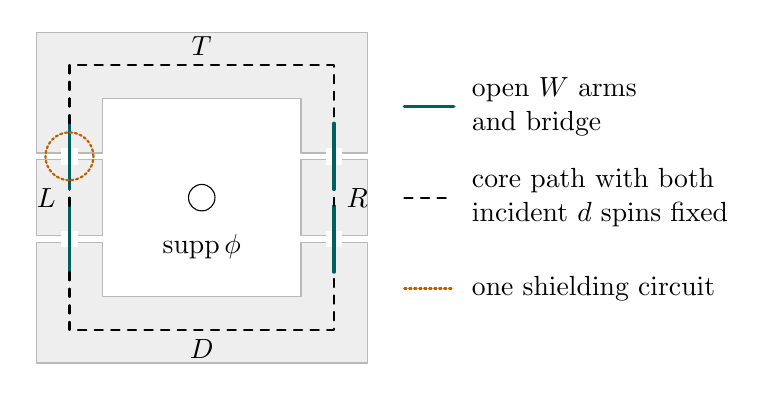
\begin{tikzpicture}[scale=1.05,line cap=round,line join=round]
 \filldraw[fill=gray!13,draw=gray!55]
  (-2,2)--(2,2)--(2,.54)--(1.2,.54)--(1.2,1.2)
  --(-1.2,1.2)--(-1.2,.54)--(-2,.54)--cycle;
 \filldraw[fill=gray!13,draw=gray!55]
  (-2,-2)--(2,-2)--(2,-.54)--(1.2,-.54)--(1.2,-1.2)
  --(-1.2,-1.2)--(-1.2,-.54)--(-2,-.54)--cycle;
 \filldraw[fill=gray!13,draw=gray!55] (-2,-.46) rectangle (-1.2,.46);
 \filldraw[fill=gray!13,draw=gray!55] (1.2,-.46) rectangle (2,.46);
 \foreach \x in {-1.6,1.6}{
  \foreach \y in {-.5,.5}{
   \fill[white] (\x-.1,\y-.1) rectangle (\x+.1,\y+.1);
  }
 }
 \draw[teal!75!black,very thick]
  (-1.6,.1)--(-1.6,.9) (1.6,.1)--(1.6,.9)
  (-1.6,-.1)--(-1.6,-.9) (1.6,-.1)--(1.6,-.9);
 \draw[black,dashed,thick]
  (-1.6,.9)--(-1.6,1.6)--(1.6,1.6)--(1.6,.9)
  (-1.6,-.9)--(-1.6,-1.6)--(1.6,-1.6)--(1.6,-.9)
  (-1.6,-.1)--(-1.6,.1) (1.6,-.1)--(1.6,.1);
 \draw[orange!75!black,densely dotted,thick] (-1.6,.5) circle (.29);
 \node at (0,1.83) {$T$};
 \node at (0,-1.83) {$D$};
 \node at (-1.88,0) {$L$};
 \node at (1.88,0) {$R$};
 \draw (0,0) circle (.16);
 \node[below=5pt] at (0,-.16) {$\supp\phi$};
 \draw[teal!75!black,very thick] (2.45,1.1)--(3.05,1.1);
 \node[right,align=left] at (3.15,1.1) {open $W$ arms\\and bridge};
 \draw[black,dashed,thick] (2.45,0)--(3.05,0);
 \node[right,align=left] at (3.15,0) {core path with both\\incident $d$ spins fixed};
 \draw[orange!75!black,densely dotted,thick] (2.45,-1.1)--(3.05,-1.1);
 \node[right,align=left] at (3.15,-1.1) {one shielding circuit};
\end{tikzpicture}
\caption{The separator after successful trial selection. Gray regions carry
complete $(s,W)$ patterns. Short bridges join the selected open arms across
the gaps; their transverse colors need not be observed. On the dashed core
portions both incident transverse spins are fixed. A surrounding circuit
protects the outside data during each bridge insertion. Only one shielding
circuit and one selected trial per gap are shown.}
\label{fig:screen-separator}
\end{figure}

\begin{lemma}[Selected-arm shielding]
\label{lem:screen-shielding}
For fixed $q$, each trial has conditional two-arm success probability
at least $p(q)>0$, given all earlier trial data. If the first successful
trial is selected, the probability that no trial succeeds is at most
$(1-p(q))^M$. The probability that the selected hole has no surrounding
plus $W$ circuit between scales $Cw$ and $R/10$ is at most $\eta(q)$,
where $\eta(q)\to0$ as $q\downarrow0$. These bounds hold after
averaging over the complete block patterns.
\end{lemma}

\begin{proof}
Reveal previous trials completely before testing the next. Their buffered
neighborhoods are disjoint, so this is exterior $(s,W)$ data for the
current trial. The tube version of \cref{prop:circuits} gives $p(q)$;
the aspect ratios are fixed once $q$ is fixed. A stack of separated
annuli between $Cw$ and $R/10$ gives circuit failure probability at most
$\eta(q)\le Cq^\alpha$ for some $\alpha>0$.

Write $A_j$ for the increasing two-arm event, $G_j$ for the surrounding
plus-circuit event, and $\mathscr H_j$ for the full previous trial
history. Positive association in the remaining law gives
\begin{equation}
 \P(A_j\cap G_j^c\mid\mathscr H_j)
 \le \eta(q)\P(A_j\mid\mathscr H_j).
 \label{eq:screen-relative-shielding}
\end{equation}
If $J$ is the first successful trial, sum this inequality over the
disjoint events $\{J=j\}$. Their total probability is at most one;
there is no factor $M$ in the resulting shielding error. Iterating the
conditional arm bound gives the failure probability. Revealing all
remaining block patterns afterward does not change either averaged
estimate. We do not assert \eqref{eq:screen-relative-shielding} after
conditioning on each individual complete pattern.
\end{proof}

Retain the original marginal law of $S_\delta$. Given this pattern,
select the first successful trial at every gap using a fixed order,
and select its two arms by a deterministic rule. For each selected pair
of arms, choose by a fixed deterministic rule a $W$-lattice path inside
the hole joining their endpoints and meeting the prescribed pattern only
at those plus endpoints. The fixed hole geometry provides such a path for
all sufficiently small meshes. On success, replace the conditional law
by the upper law obtained by pinning these paths open and plus. The new
conditional law is therefore well defined, and its bridge pins are
functions of $S_\delta$.
On unsuccessful patterns leave the conditional law unchanged, couple it
identically to the original law, and take no core-color observations.
Call the resulting law $\mathbb Q_\delta$.

\begin{lemma}[Bridge coupling and exact separation]
\label{lem:screen-bridge-coupling}
The laws $\P_\delta$ and $\mathbb Q_\delta$ can be coupled with their
block patterns identical. Except on probability at most $4\eta(q)$,
their insertion, full exterior data, and all $d$ colors at core sites
outside the shielding disks agree, on the event that all four gaps
have successful trials. Under $\mathbb Q_\delta$, on that success
event one can choose pattern-measurable core paths and condition on
their incident $d$ sites so that the insertion and the full exterior
are conditionally independent given $Y_\delta=(S_\delta,C_\delta)$.
\end{lemma}

\begin{proof}
Fix a block pattern $S$, and write $H(S)$ for success at all four gaps.
On this event let $G_i(S)$ be the plus-circuit event around the selected
hole at gap $i$, and let $\mu_i^S$ be the conditional law after the first
$i$ selected bridges have been pinned, with $\mu_0^S$ the original
conditional law. On unsuccessful patterns put $\mu_i^S=\mu_0^S$ and
$G_i(S)=\Omega$. For two successive laws use the monotone stopping
coupling of \cref{prop:comparison}, searching outward from the newly
pinned hole inside its shielding disk. Stop at the disk's outer boundary
and declare this adjacent coupling unsuccessful if no surrounding plus
circuit has been found. All previously inserted pins are identical in
these two laws.
In the lower law the first plus circuit surrounding that hole is also
open in the upper law. All changed data are inside this common cut. By
\cref{lem:finite-cuts}, the configurations outside it can be sampled
identically, including complementary-component colors. In particular
their exterior color connections are unchanged. The exact neutrality of
the insertion removes any change in the chosen additive height anchor.
If $G_i(S)$ occurs in the lower law, this cut is found inside the
shielding disk, so the required insertion, exterior data, and core colors
outside that disk agree.

To realize these adjacent couplings in the plane, first run each disk-stopped
search in finite flat exhaustions at fixed $\delta$ and $S$, retaining a
binary failure marker. Each conditioning event involves finitely many
prescriptions and has positive plane probability. To verify positivity,
place $S$ and the compatible bridge pins in a larger buffered flat box
with an open plus $W$ perimeter. Keep every prescribed state, put plus
on all remaining $s$ sites, close all remaining interior $W$ edges, and
take all $d$ spins equal. Every factor in \cref{eq:spatial-edge-weight}
is positive because $t\in[1/2,1)$. Let $\mu_{\mathrm{box}}$ denote the
flat law in this box. The restriction $p$ of this filling to a regular
inner core containing the prescriptions is a complete pattern with
$\mu_{\mathrm{box}}(p)>0$. The upper bound
$\mu_{\mathrm{box}}(p)\le C\pi(p)$ in \cref{prop:pattern-comparison}
gives $\pi(p)>0$, and hence positive plane probability for the conditioning
event containing it.

The conditional marginals therefore converge on cylinder events. Extract
a joint limit on the countable product of spin and edge coordinates,
together with the failure marker. Its probability bound passes to the limit,
as does equality of each fixed exterior coordinate on success. Taking their
countable intersection gives equality of the full exterior configuration;
its computable height increments agree as well. Thus this limit has the
plane marginals and the coupling properties just proved in finite volume.

For fixed $S$, the event $G_i(S)$ is now fixed and increasing. The previous
plus pins can only increase its probability. With $\E_S$ denoting
expectation over the original pattern marginal, this gives
\[
 \E_S\!\left[\ind_{H(S)}
       \mu_{i-1}^S\bigl(G_i(S)^c\bigr)\right]
 \le
 \E_S\!\left[\ind_{H(S)}
       \mu_0^S\bigl(G_i(S)^c\bigr)\right]
 \le \eta(q).
\]
The first inequality is the comparison at each fixed pattern; the second
is \cref{lem:screen-shielding} after averaging over the selected trial.
At a fixed mesh the pattern space is finite, so choose these adjacent
conditional couplings measurably in $S$. Apply the displayed estimate to
each of their marginal failure probabilities, then glue the four couplings
and use a union bound. Their searches stay in disjoint buffers, and every
intermediate law retains the original pattern marginal. This proves the
asserted joint coupling.

On a successful pattern, join the outer arm ends through compact cores
of the blocks. The core portions together with the open arms and the
new bridges give a closed walk winding once around $B$ and lying inside
$Q$. Extract a simple winding cycle, with its lattice-width incident
sites, by deterministic loop erasure. On every non-open core edge,
condition on both incident $d$ sites; include the incident sites at the
transitions. Along the arms and bridges no $d$ observation is needed.
Indeed the local factor there is $t\ind_{s_i=s_j}$, independent of
transverse colors. Along a remaining core edge all its $s,W$ data and
the two incident $d$ values are fixed. Every local factor crossing the
cycle is consequently either fixed or independent of the transverse
variables. The Gibbs weight factors into an inside weight and an
outside weight after these observations. This proves conditional
independence. This factorization is made with colors as actual spin
variables, before summing them into cluster-count factors; no hidden
connectivity weight remains across the separator. All observed $d$
sites lie in the compact cores and outside the shielding disks.
\end{proof}

\begin{proof}[Proof of \cref{prop:screened-orthogonality} in the plane]
Truncate the insertion to $[-T,T]$, writing the result as
$X_\delta^{(T)}$, and set
\[
 r(T)=\sup_\delta\E_{\P_\delta}
             |X_\delta-X_\delta^{(T)}|.
\]
The moment bound gives $r(T)\to0$. Suppose the coupling mismatch
probability is $\varepsilon$, and the unsuccessful-pattern probability
is $\zeta$. Duality against bounded functions gives
\begin{align}
 \|\E_{\P_\delta}[X_\delta^{(T)}\mid\mathscr E_\delta]\|_1
 &\le
 \|\E_{\mathbb Q_\delta}
            [X_\delta^{(T)}\mid\mathscr E_\delta]\|_1
       +2T\varepsilon\notag\\
 &\le
 \|\E_{\mathbb Q_\delta}[X_\delta^{(T)}\mid Y_\delta]\|_1
       +2T\varepsilon+2T\zeta\notag\\
 &\le
 \|\E_{\P_\delta}[X_\delta^{(T)}\mid Y_\delta]\|_1
       +4T\varepsilon+2T\zeta.
 \label{eq:screen-bounded-coupling}
\end{align}
For the middle inequality use conditional independence on success and
bound the unsuccessful histories by their probability times $2T$.
The outer inequalities use agreement of the joint insertion and
conditioning data. They do not require equal laws of $Y_\delta$.

By \cref{lem:screen-core-colors}, at each fixed layout the final
conditional norm has limsup at most $r(T)$. The coupling and trial
lemmas give $\varepsilon\le4\eta(q)$ and
$\zeta\le4(1-p(q))^M$. Returning from $X_\delta^{(T)}$ to $X_\delta$
therefore gives
\[
 \limsup_{\delta\downarrow0}
 \|\E[X_\delta\mid\mathscr E_\delta]\|_1
 \le 2r(T)+16T\eta(q)+8T(1-p(q))^M.
\]
Given an error tolerance, first fix $T$ large, then $q$ small, then
$M$ large, and finally fix a layout as in \eqref{eq:screen-scale-order}.
Taking its mesh limit proves \eqref{eq:plane-exterior-orthogonality}.
Only original-law moments have been used; there is no moment assumption
for the artificially pinned law.
\end{proof}

\subsection{Transfer to flat domains}

\begin{proof}[Completion of the proof of
\cref{prop:screened-orthogonality}]
Choose a regular, fixed-width spin ring $A$ between the insertion and
$\partial Q$, with positive clearance from both. Let $R_\delta$ denote
both spins on a lattice-width enlargement of this ring. For a ring
assignment $r$ admitting an interior filling, let $\mathsf K_\delta^r$
be the finite interior spin Gibbs kernel obtained from
\cref{eq:spin-constraint,eq:spin-weight}, with $r$ fixed on the ring and
all factors meeting the interior retained. Define
\[
 g_\delta(r)=\int X_\delta\,\dd\mathsf K_\delta^r,
\]
and put $g_\delta(r)=0$ when no interior filling is admissible.
The neutral insertion is determined by the interior height increments,
so its value in this formula is independent of an additive height anchor.
The finite product weights give this same conditional interior kernel in
every flat domain; the identity also passes from flat exhaustions to the
plane on cylinder events. Thus $g_\delta(R_\delta)$ is a version of the
conditional mean of $X_\delta$ under each of these laws, including on
admissible ring assignments that may have zero plane probability. All
these expectations are finite at each mesh.

Apply the separated-block proof to a slightly smaller surrounding square,
whose exterior contains the ring. All its strict projection clearances
persist under this small change of the surrounding square. Since the ring
data belong to that exterior sigma-field, conditional Jensen gives
$\E_{\P_\delta}|g_\delta(R_\delta)|\to0$, hence convergence in plane
probability. The uniform full-spin
contiguity of \cref{prop:full-contiguity}, on a fixed larger box,
transfers this convergence in probability to the flat laws, even for
mesh-dependent tests of the ring data. The neutral moment estimate in
\cref{lem:screen-pattern-moments}, with no patterns, gives uniform
integrability of these conditional means by conditional Jensen.
Consequently their absolute means tend to zero uniformly over the
flat laws. Finally the Markov property across the ring gives
\[
 \E[X_\delta\mid\mathscr E_\delta(Q)]
    =\E[g_\delta(R_\delta)\mid\mathscr E_\delta(Q)],
\]
and conditional Jensen proves the asserted exterior estimate. Uniformity
can equivalently be checked by taking an arbitrary contradicting
sequence of flat domains; all buffers remain fixed and the same argument
applies. At a random exact cut, the statement is used for the realized
conditional flat law. Subsequent conditioning is not included in this
claim.
\end{proof}

In particular, if finitely many spectator height differences or heights
anchored on an exterior wall are evaluated along paths outside $Q$,
their bounded functions are legitimate exterior observables. Unbounded
products are handled by the moment estimates of the next section. This
is the conditional harmonicity input, with no box shrinking at the
lattice scale.

\section{Flat-domain Gaussian limits}
\label{sec:gaussian}

We prove the Gaussian limit for the unit-increment height
\(K_\delta=2H_\delta\), first in deterministic flat chambers and then
conditionally in chambers produced by a stopping exploration. The uniformity
in the chamber is what permits the second use.

Every chamber in this section is an accessible component behind a connected
matching \(W\) perimeter, with the medial resolution at pinches from
\cref{lem:finite-cuts}. Its open face domain is simply connected. The
perimeter carries its actual wire, and incident faces are not joined across a
pinch. We subtract its constant height. For the moment arguments choose \(N\)
to be the free current complementary to this wall percolation \(W\); all its
interior components then have fair colors. The initial flat domain is
included by taking \(N\) to be the free dual current. Either corner parity
may carry the wall.

A collection of chambers will always have pairwise disjoint open interiors;
their closures may touch. Sample their centered flat laws independently,
patch the fields on these disjoint cell interiors, and set the field to zero
on the exposed complement. Let \(U_\delta\) denote their open union. Fix an
open disk \(B_0\) containing all chamber closures with a fixed outer margin,
and put
\[
             F_\delta=\overline B_0\setminus U_\delta.
\]
Thus \(F_\delta\) is the closed complement in a common compact ambient set.
Hausdorff convergence of these \(F_\delta\) is equivalent here to local
Hausdorff convergence of the closed complements in the plane. Constants may
depend on \(B_0\), the fixed parameter, and the moment order, but not on the
shapes or the number of chambers.

\begin{theorem}[Flat-domain limit]\label{thm:flat-gff}
Let \(U_\delta\) be a single deterministic flat chamber, or a finite
mesh-dependent union of independent chambers with pairwise disjoint
interiors, as above. Suppose \(F_\delta\) converges in Hausdorff distance to
\(F\), and set \(U=B_0\setminus F\). Then
\[
                K_\delta\ \Longrightarrow\ h_U/a
             \quad\text{in }H^s_{\mathrm{loc}}(U),\qquad s<-1,
\]
where the restrictions of \(h_U\) to the components of \(U\) are independent
zero-Dirichlet GFFs with logarithmic singularity \(-\log|x-y|\). All finite
joint smooth-test moments with supports in \(U\) converge. Different limiting
components are independent even if their discrete precursors were the same
chamber. Either wall parity and either atomic or interpolated smearing gives
the same limit. The fields extended by zero off \(U_\delta\) are uniformly
tight in \(H^s_{\mathrm{loc}}(B_0)\) for every \(s<-1\).
\end{theorem}

The proof first bounds all moments and their boundary traces. Screened
orthogonality then makes the limiting moments harmonic away from collisions;
a local neutral-pair comparison identifies their logarithmic poles and hence
their Wick recursion. We determine its coefficient from the plane limit
before completing the theorem. The last proposition turns the deterministic
result into the conditional statement needed for stopped explorations.

\subsection{Limiting chambers and their Green kernels}

For an open set \(V\) whose components are simply connected, write \(G_V\)
for the Dirichlet kernel with logarithmic singularity \(-\log|x-y|\) in
each component, extended by zero between different components and when
either argument lies outside \(V\). For tests put
\[
 G_V(f,g)=\iint f(x)G_V(x,y)g(y)\,\dd x\,\dd y.
\]
The planar connected-complement criterion shows that \(F_\delta\) above is
connected: an open subset of the sphere has simply connected components
exactly when its complement is connected. This uses disjoint interiors, not
disjoint closures. The next lemma supplies the boundary facts used twice
below, first in Wick's rule and then in the conditional limit.

\begin{lemma}[Connected complements and Green convergence]
\label{lem:flat-green-geometry}
Let \(F_n\) be connected compact subsets of \(\overline B_0\) containing
\(\partial B_0\), and suppose \(F_n\to F\) in Hausdorff distance. Put
\(V_n=B_0\setminus F_n\) and \(V=B_0\setminus F\). Every component of
\(V_n\) and \(V\) is simply connected, every compact subset of \(V\) is
eventually contained in \(V_n\), and
\[
                G_{V_n}(x,y)\longrightarrow G_V(x,y)
\]
locally uniformly for distinct \(x,y\in V\), including when they lie in
different components of \(V\).
The zero-extended kernels satisfy \(0\le G_{V_n},G_V\le G_{B_0}\).
As a function of the closed complement and its two arguments, this
zero-extended Green kernel is Borel measurable.

For any proper simply connected domain \(W\), with
\(d_W(x)=\dist(x,\partial W)\), one has
\begin{equation}
 0\le G_W(x,y)\le
       4\sqrt{\frac{d_W(x)}{|x-y|}}
 \quad\text{if }d_W(x)\le\frac{|x-y|}{16}.
 \label{eq:flat-green-boundary}
\end{equation}
In particular these Green kernels have zero boundary trace without a
boundary smoothness assumption.
\end{lemma}

\begin{proof}
Adjoin the exterior of \(B_0\) in the sphere. The complements remain
connected, and so does their Hausdorff limit. The planar criterion just
stated gives simple connectivity of every open component. Hausdorff
convergence of compact sets gives uniform convergence of their distance
functions, which proves compact containment.

For the estimate, choose a conformal map \(f:\mathbb D\to W\) with
\(f(0)=x\), and write \(f(z)=y\). The growth bound and the quarter theorem
recalled in \cref{sec:conformal-growth} give
\[
 |x-y|\le |f'(0)|\frac{|z|}{(1-|z|)^2}
          \le \frac{4d_W(x)}{(1-|z|)^2}.
\]
Under the stated hypothesis this implies \(|z|\ge1/2\). The conformal
Green identity and \(-\log t\le2(1-t)\) for \(1/2\le t\le1\) now give
\cref{eq:flat-green-boundary}.

For convergence, domain monotonicity gives the common bound
\(0\le G_{V_n}\le G_{B_0}\), with zero understood between components.
The upper kernel is bounded on compact sets away from the diagonal and
has only an integrable logarithmic singularity on the diagonal. Fix \(y\in V\) and a
component \(C\) of \(V\). On compact subsets of \(C\setminus\{y\}\),
harmonic compactness gives subsequential limits in the first variable.
If \(y\in C\), a fixed disk about \(y\) is eventually contained in one
component of \(V_n\). On that disk subtract \(\log(1/|x-y|)\).
The difference is harmonic and uniformly bounded on a fixed interior
circle by the common upper bound; the Poisson formula therefore preserves
the unit logarithmic pole in the limit. If \(y\notin C\), there is no pole.

For \(x\in V_n\), its distance to the boundary of its component equals
\(\dist(x,F_n)\). Passing \cref{eq:flat-green-boundary} to a subsequential
limit shows that this limit has zero trace on \(\partial C\), since
\(\dist(x,F_n)\to\dist(x,F)\). The maximum principle now identifies it
as \(G_C(\,\cdot\,,y)\) when \(y\in C\), and as zero when \(y\notin C\).
The removable difference is bounded near its pole and near the boundary,
so the maximum principle applies on the whole component. Every
subsequential limit is the same. Interior harmonic estimates in both
variables give the asserted local uniform convergence. The common
logarithmic upper bound also gives convergence of \(G_{V_n}(f,g)\) for
fixed smooth tests with supports compactly contained in \(V\).
On the space of connected complements, the local uniform assertion gives
continuity of \(G_{B_0\setminus F}(x,y)\) where \(x,y\notin F\) and \(x\ne y\).
These positive-clearance sets form a countable cover of the interior
off-diagonal pairs. Extension by zero off the open set and the usual
diagonal value therefore give a Borel kernel, and hence Borel smeared
covariances.
\end{proof}

\subsection{Moments and boundary traces}

Choose once \(R_0>2\diam(B_0)\).

\begin{proposition}[Logarithmic moments]
\label{prop:log-moments}
Let $z_1,\ldots,z_{2m}$ be corner-grid sites in a flat chamber of
diameter at most $R_0/2$. They may lie on either parity. Then
\begin{equation}
 \left|\E\prod_{i=1}^{2m}K(z_i)\right|
 \le C_m\sum_{\mathcal P}\prod_{\{i,j\}\in\mathcal P}
 \left(1+\log^+\frac{R_0}{|z_i-z_j|\vee\delta}\right),
 \label{eq:flat-log-moments}
\end{equation}
where the sum is over pairings. Odd moments vanish. The same bound holds for
independent flat chambers after setting the field to zero off those chambers.
For a compactly supported bounded test $f$, uniformly over all such chambers,
\begin{equation}
 \E|K_\delta(f)|^{2m}\le C_m\|f\|_\infty^{2m}.
 \label{eq:flat-smearing-moments}
\end{equation}
For any fixed smooth compactly supported profile $f$, put
$f_{r,z}(x)=r^{-2}f((x-z)/r)$. If $0<\delta\le r$, then
\begin{equation}
 \E|K_\delta(f_{r,z})|^{2m}
       \le C_{m,f}\left(1+\log^+\frac{R_0}{r}\right)^m.
 \label{eq:flat-scaled-moments}
\end{equation}
This includes a mass-one smooth average of radius $r$ for a fixed profile.
\end{proposition}

\begin{proof}
Condition on the current $N$ and the $s$ spins. By \cref{lem:finite-cuts},
the centered height at a wall-parity site is a sum of jumps of size two with
independent fair signs, one sign per contributing cluster. A cluster's
coefficient at a site is zero or has absolute value two. Its sign is shared
by all its odd holes.

The same signed expansion controls opposite-parity sites. For such a site
$x$, choose an incident wall-parity site $v$, and let $C_x$ be the free
$N$ component containing $x$. The corner rule gives
\[
          K(x)=K(v)+\varepsilon_W s(v)d(C_x),
\]
where the fixed sign $\varepsilon_W$ records which parity carries $W$.
Absorb this term into the coefficient of $d(C_x)$. Conditional on $(N,s)$,
every height is still a sum of the independent fair component colors,
now with coefficients of absolute value at most three. If a component has
a nonzero coefficient at a site, that site lies in the component or its
filled hull up to distance $O(\delta)$: wall-parity contributions come from
odd holes, and the extra contribution is incident to the component.
Consequently a component shared by two sites has diameter at least their
separation minus $O(\delta)$.

Expanding an even product and summing the independent signs leaves only
terms in which every sign appears an even number of times.
Pair the occurrences of each such sign. Overcounting by all pairings gives
an upper bound by $C_m$ times sums of products of shared-cluster counts
$M(z_i,z_j)$. This argument does not assert independence of the counts.

A contributing cluster surrounds or is incident to the relevant site.
The preceding support observation gives the required diameter lower bound
for a shared cluster. At a fixed site only boundedly many components of
diameter at most $C\delta$ can contribute, including isolated vertices;
put all of these contributions in the lattice cutoff. Above that cutoff,
a fixed number of boxes at a cluster's diameter scale detect its passage
or enclosure. By
\cref{prop:cluster-counts}, the count in each such dyadic shell has uniformly
bounded moments of every fixed order. Minkowski's inequality therefore gives
\[
 \|M(z_i,z_j)\|_{L^m}
 \le C_m\left(1+\log^+\frac{R_0}{|z_i-z_j|\vee\delta}\right).
\]
Holder's inequality for the product of the $m$ counts proves
\cref{eq:flat-log-moments}. Height reflection about the flat value proves
vanishing of odd moments. The argument is unchanged in several independent
chambers; shared-cluster counts between different chambers are zero.

Integrate the estimate against the interpolation weights, or the atomic
Riemann weights, of the tests. Each logarithmic factor is uniformly
integrable in its two variables, including its lattice diagonal: the latter
contributes $O(\delta^2\log(1/\delta))$. Since the pairs have disjoint sets
of variables, this proves \cref{eq:flat-smearing-moments}. Rescaling a
fixed profile by $x=z+ru$ gives \cref{eq:flat-scaled-moments}. Here
$\delta/r\le1$ is essential for an atomic smearing: after the rescaling
the diagonal part has the additional uniformly bounded factor
$(\delta/r)^2\log(r/\delta)$, while the common scale contributes
$1+\log^+(R_0/r)$.
\end{proof}

\begin{proposition}[Boundary decay]
\label{prop:boundary-decay}
Consider deterministic flat chambers in a fixed bounded region, with
connected accessible walls, and a Hausdorff limit of their complements.
For any limiting open component, moment kernels obtained from
\cref{eq:flat-log-moments} have zero boundary trace in a distinguished
variable when the other variables remain at distinct interior points.
The bounds and the trace conclusion are uniform for the discrete chambers.
More precisely, a shared cluster joining the height contribution at a site
within distance $r$ of a matching connected wall to one at distance at least
$R$ from that site has probability at most $C(r/R)^\eta$, with fixed
positive outer clearance and $\delta\le r\ll R$.
\end{proposition}

\begin{proof}
The relevant wall component reaches from the small scale to the outside of
the fixed testing window. A shared cluster either is incident to the
distinguished site or encloses it. In the incident case its connected
passage reaches the outer scale forced by the distant spectator. In both cases it must
avoid matching circuits attached to this wall at every scale between
$r$ and $R$: such a circuit separates the distinguished contribution
from the distant one. The conditional circuit estimate in \cref{prop:circuits}
gives a uniformly positive success probability at a fixed fraction of these
separated scales. An attached circuit blocks the cluster, so iteration gives
$C(r/R)^\eta$. The argument is within the accessible chamber with its wire
retained; no regularity of the geometric wall is used.

In every pairing contributing to a mixed even moment, the distinguished
site is paired with one spectator. The corresponding shared cluster has
a fixed positive minimum diameter. Its count, restricted to surviving the
attached-circuit trials, tends to zero in every smaller $L^p$ norm: apply
Holder to the survival indicator and the higher count-moment bound from
\cref{prop:cluster-counts}. The remaining counts are bounded by
\cref{eq:flat-log-moments}. This proves vanishing of the mixed moment as
the distinguished site approaches the wall. For fixed distinct spectators
the pairing bound itself is uniformly bounded near the wall. Smearing first
at a radius smaller than the site's wall distance gives the same result
for distributional moment limits. Once harmonicity is established below,
the mean-value property identifies these smearing limits with the pointwise
boundary trace. The proof also applies when the wall develops a pinch:
only the actual connected wall crossing the testing scales is used.
\end{proof}

\begin{lemma}[Parity and interpolation]
\label{lem:parity-interpolation}
On compact subsets with positive clearance from the wall, the two parity
smearings of $K$, and their smooth nodal interpolation, have the same
subsequential distributional limits and the same joint test moments.
Here each original parity has Riemann weight $\delta^2$; the combined
corner grid has weight $\delta^2/2$ per site. Thus its interpolation is
compared to the average of the two parity smearings, not their sum.
\end{lemma}

\begin{proof}
Pair each site of one parity with an incident site of the other parity by a
fixed lattice translation. The paired height difference is $Z_e\in\{-1,1\}$.
Conditional on $(N,s)$ it is, up to a deterministic orientation, a fixed
$s$ spin times the fair color of the adjacent $N$ component. Thus for two
well-separated paired edges,
\[
 |\E[Z_eZ_{e'}]|\le
 \P(\text{their adjacent sites belong to the same }N\text{ component}).
\]
A matching $W$ circuit around the first edge separates these components.
Bulk circuit trials between the lattice scale and their separation imply
that, for separation at least $r$ and fixed wall clearance,
$|\E[Z_eZ_{e'}]|\le C(\delta/r)^\eta$. This is equivalently the conditional
fair-color coupling in disjoint pin-free buffers. In particular it does not
infer smallness merely from the deterministic bound $|Z_e|=1$.

For a smooth test, the variance of its averaged paired differences is bounded
by $C r^2+C(\delta/r)^\eta$: separate pairs at distance below $r$ from all
other pairs. First let $\delta$ decrease to zero and then let $r$ decrease
to zero. Changing the test's evaluation point within a paired cell gives an
$O(\delta)$ smooth-test error in $L^2$ by
\cref{eq:flat-smearing-moments}. This proves convergence of the difference
to zero in $L^2$. Uniform higher moments and interpolation give convergence
in every finite $L^p$. Nodal interpolation is an average of the same local
pairings with smooth weight errors, so the argument includes it.
\end{proof}

\begin{lemma}[Tightness and absence of collision measures]
\label{lem:flat-tightness}
Centered flat heights are tight in $H^s_{\mathrm{loc}}$, for every $s<-1$,
uniformly over the chambers above. Every finite joint test moment converges
along distributional convergence. Once the limiting moment distributions
are harmonic off their collision diagonals, their smooth representatives
there represent the full distributions: there are no additional measures
or distributions supported on those diagonals.
\end{lemma}

\begin{proof}
Put a cutoff $\chi$ in a fixed square regarded as a torus, with normalized
Fourier basis $e_n$. The uniform second-moment bound for
$K_\delta(\chi e_n)$ is independent of $n$. Hence, for $q>1$,
\[
 \sup_\delta\E\|\chi K_\delta\|_{H^{-q}}^2
 \le C\sum_{n\in\Z^2}(1+|n|^2)^{-q}<\infty.
\]
For $1<q<-s$, compactness of $H^{-q}\hookrightarrow H^s$ gives tightness.
Use a countable exhaustion of cutoffs and summable exceptional probabilities.
Higher versions of \cref{eq:flat-smearing-moments} give uniform
integrability of all finite test products, proving convergence of moments.
These statements also hold for a finite independent collection of chambers or
for fields set to zero on their already exposed complement.

Here is a direct verification of the last assertion, independent of any
pointwise choice on diagonals. Mollify each variable of a $j$th moment
distribution at the same radius $r$. For each fixed $r$ the mesh limit is
taken first, so eventually $\delta\le r$. Holder and
\cref{eq:flat-scaled-moments} bound the mollified kernel by
$C_j(1+|\log r|)^{j/2}$ on compact sets, even at collisions. Away from
pairwise distances at most $2r$, separate harmonicity and radial mollifiers
make it exactly the smooth unmollified kernel. Taking the mollification
radius to be a fixed fraction of the smallest pair distance also bounds
that kernel by a power of its logarithm. The collision neighborhood has
volume $O(r^2)$, so both integrals over it tend to zero. The mollified kernels
therefore converge locally in $L^1$ to the smooth kernel extended across
the diagonals. Their distributional limit is the original moment
distribution, proving the assertion.
\end{proof}

\begin{lemma}[Centered remainders on small revealed sets]
\label{lem:small-set-remainders}
Conditional on a stopped exploration using \cref{lem:finite-cuts}, let
$R_\delta$ be its centered flat remainders, set to zero on exposed sites.
Let $E_\delta$ be a set of sites measurable in the stopped data, in a fixed
bounded region,
and write $m_\delta$ for the area of their lattice cells. If
$m_\delta\to0$ in probability, then, for every bounded deterministic test $f$,
\[
           R_\delta(f\ind_{E_\delta})\longrightarrow0
                           \quad\text{in }L^2.
\]
The conclusion is uniform over the stopped geometries. An additional
revealed mean bounded by a fixed constant has a vanishing contribution on
these sets as well.
\end{lemma}

\begin{proof}
Condition on the stopped data and apply the second-moment case of
\cref{prop:log-moments}. If the ambient diameter is at most $R_0$, a
rearrangement bound for the logarithmic kernel gives
\[
 \E\bigl[|R_\delta(f\ind_{E_\delta})|^2\mid\mathcal E_\delta\bigr]
 \le C\|f\|_\infty^2 m_\delta^2
          \left(1+\log^+\frac{R_0^2}{m_\delta}\right),
\]
with value zero at $m_\delta=0$. To verify the discrete bound, for each
fixed site sum the decreasing logarithmic kernel first over its nearest
$O(m_\delta/\delta^2)$ cells, allowing the fixed cell-area factor of either
parity. A disk of radius comparable to
$\sqrt{m_\delta}$ bounds this sum by
$C m_\delta(1+\log^+(R_0^2/m_\delta))$; its central cell uses the cutoff
$|x-y|\vee\delta$. Sum once more over $E_\delta$. The right side is a
bounded function of $m_\delta$ tending to zero at zero, so averaging proves
the claim. A mean bounded by $M$ contributes at most
$M\|f\|_\infty m_\delta$. In particular the lemma applies to shrinking
neighborhoods of an explored set once their areas have been shown to vanish;
it does not presume that area estimate or thinness.
\end{proof}

\subsection{Harmonic moment kernels and their collision coefficients}

Fix a subsequence along which the flat fields and their moment
distributions converge, and extract the plane covariance on the same
subsequence. Write $\kappa>0$ for the coefficient denoted by $\beta$ in
\cref{prop:plane-green}:
for smooth compactly supported tests $\alpha,\beta$ of integral zero,
\begin{equation}
 \lim_{\delta\downarrow0}
 \E[K^{\mathrm{pl}}_\delta(\alpha)
       K^{\mathrm{pl}}_\delta(\beta)]
 =\kappa\iint\alpha(x)\beta(y)\log\frac1{|x-y|}\,\dd x\,\dd y.
 \label{eq:subsequential-kappa}
\end{equation}
At this stage $\kappa$ may depend on the subsequence. In particular,
neither Gaussianity nor the final normalization is being assumed.

The complementary open limit \(U\) may have several components even when
their discrete precursors belong to one component. Let \(T_j\) denote a
subsequential \(j\)th moment distribution on \(U^j\), with \(T_0=1\).
Their existence and convergence against test products follow from
\cref{lem:flat-tightness}.

We explain why separated spectator heights are legitimate exterior
observations in the first application of screening. Localize the Laplace
test to a disk \(B\), and choose \(B,Q,Q^+\) concentric, with squares
\(Q\Subset Q^+\), so that the radius of \(B\) is less than one thousandth
of the side of \(Q\).
Choose \(Q^+\) compactly inside the limiting component containing \(B\),
disjoint from the spectator disks. An arbitrary local harmonicity test can be
partitioned into tests with such small supports. Fix a simple curve surrounding \(Q\)
inside \(Q^+\setminus\overline Q\), at positive distance from both
boundaries. For all sufficiently fine meshes, choose a simple corner-grid
approximation \(\Gamma_\delta\) of this curve in the discrete chamber and
outside \(Q\).

A spectator in that chamber is read by summing corner increments from
its flat wall. Start with any such path. If it enters \(Q\), replace the
portion between its first and last encounters with \(\Gamma_\delta\) by
an arc of \(\Gamma_\delta\). The resulting path stays outside \(Q\). This
also works for spectators in a different limiting component of the same
discrete precursor. Spectators in other independently sampled chambers
may be adjoined to the exterior sigma-field: independence preserves the
screened conditional-mean bound. Thus a bounded function of all these
wall-anchored spectators is an allowed exterior observable.

On a product of disjoint interior disks, truncate the spectator product,
apply \cref{prop:screened-orthogonality}, and remove the truncation by
Holder's inequality and the higher moment bounds. This gives
\[
                     \Delta_{x_i}T_j=0\qquad(1\leq i\leq j).
\]
Summing these equations gives an elliptic equation on the product space.
Thus $T_j$ has a smooth,
separately harmonic representative off the diagonals.
\cref{lem:flat-tightness} now excludes any additional distribution on the
diagonals. Flat height
reflection gives $T_1=0$. The logarithmic moment bound and
\cref{prop:boundary-decay} apply to these representatives, by averaging
on disjoint circles. They give, respectively, polylogarithmic growth
at a collision and zero boundary trace in each variable away from the
other insertions.

\begin{lemma}[Uniform logarithmic expansion]
\label{lem:log-singularity}
If $(y,\mathbf z)$ is a collision-free list of interior points, then,
near $x=y$,
\begin{equation}
 T_j(x,y,\mathbf z)
   =L_j(y,\mathbf z)\log\frac1{|x-y|}
       +R_j(x;y,\mathbf z),
 \label{eq:logarithmic-expansion}
\end{equation}
where $R_j$ extends harmonically in $x$ across $y$. The coefficient
$L_j$ is smooth in all its arguments. On a compact set of allowed
$(y,\mathbf z)$, the expansion holds on a common radius, and the
remainder and each fixed order of its $x$-derivatives are uniformly
bounded on a smaller common radius.
\end{lemma}

\begin{proof}
A harmonic function on a punctured disk has constant angular mode
$a+b\log r$ and nonconstant modes $a_n r^n+b_n r^{-n}$, $n\geq1$.
Polylogarithmic growth forces every $b_n$ to vanish. This proves the
expansion and removability of its remainder. To obtain parameter
uniformity, choose a fixed radius $q$ avoiding all other insertions.
The coefficient is the outward flux
\begin{equation}
 L_j(y,\mathbf z)
 =-\frac1{2\pi}\int_{|w-y|=q}
                      \partial_{n_w}T_j(w,y,\mathbf z)\,\dd s_w.
 \label{eq:collision-flux}
\end{equation}
After writing $w=y+q\exp(i\vartheta)$, the integrand varies smoothly
on a collision-free compact set. This proves smoothness of $L_j$.
Subtract its logarithm from the boundary values on the circle and
apply the Poisson formula. Interior derivative estimates give the
claimed uniform bounds on $R_j$. This obtains uniformity from a
fixed circle, not from a potentially nonuniform singular limit.
\end{proof}

We next state the precise local independence needed to read this flux.
For a smooth test $\alpha$, put
$\alpha_r(x)=r^{-2}\alpha((x-y_0)/r)$. For the neutral insertions below,
use the bilinear nodal smearing of \cref{sec:spectral} in both the flat and
plane laws. Its coefficient array has exactly zero sum, and this is
precisely the discretization in \cref{eq:subsequential-kappa}.
In flat chambers \cref{lem:parity-interpolation} identifies this choice
with either parity smearing.

\begin{lemma}[A neutral pair and distant observations]
\label{lem:neutral-pair-mixing}
Fix an interior disk $B(y_0,4R)$ and a finite family of spectator
tests supported outside it. Let $Y_\delta$ be a product of the
corresponding flat height averages, or of smoothed plane increments.
If $\alpha,\beta$ are smooth zero-integral tests in disjoint bounded
disks, then
\begin{align}
 \lim_{r\downarrow0}\limsup_{\delta\downarrow0}
 \big|&\E[K_\delta(\alpha_r)K_\delta(\beta_r)Y_\delta]
 \notag\\[-1mm]
 &-\E[K^{\mathrm{pl}}_\delta(\alpha_r)
                   K^{\mathrm{pl}}_\delta(\beta_r)]\,
                      \E Y_\delta\big|=0.
 \label{eq:neutral-factorization}
\end{align}
For flat fields, the assertion is uniform over patched collections in a
common bounded region for which the local chamber contains this disk and
every spectator buffer lies in its assigned chamber. All boundary constants have been
subtracted. Spectators in other independently sampled pieces are allowed.
\end{lemma}

\begin{proof}
Here are the stopping and coloring details of the coupling. Rescale
$R$ to one and take $\rho=r^{1/2}$; all sufficiently small $r$ have
both local supports in $B(y_0,Cr)\subset B(y_0,\rho)$.
Search inward using only $(s,W)$ for a monochromatic open $W$ circuit
in the stack of annuli between radii $\rho$ and $R$. The search stops
on the first complete circuit and does not inspect its interior.
By \cref{prop:circuits,prop:comparison}, the probability of exhausting
the stack without finding a circuit is at most $C\rho^\eta$, for
some $\eta>0$. The exponent and constants depend on the fixed model
parameter and the buffered shapes, not on the flat domain.

On success reveal the entire exterior of the stopped circuit,
including its transverse colors. No $N$-cluster crosses an open
$W$ circuit, so this revelation determines the outside color
identifications without imposing an interior color constraint.
By \cref{lem:finite-cuts}, the unexplored interior is a flat law,
with its constant $s$ boundary value and independent fair colors on
its free $N$-clusters. The sign of the wall causes no change to the
law of neutral height increments: reflect a spin sign if necessary.

The spectator heights are measurable in the revealed exterior.
For a bounded flat piece, read each of them by summing corner
increments from its prescribed wall along paths avoiding
$B(y_0,R)$. Such paths exist: any path entering this interior disk
can be detoured through an annulus contained in the domain. The
same detour works in all sufficiently fine approximations, and
averaging uses only nearby exterior sites. For plane increments,
choose the integration paths between their two spectator buffers
outside the disk. Thus we have not conditioned on absolute heights
before obtaining a genuine stopping cut.

Inside the circuit apply the common-cut monotone coupling from
\cref{prop:comparison,prop:circuits} to the flat law and the plane
law. Between scales $Cr$ and $\rho$ there are order
$\log(\rho/r)$ buffered trials. Each successful common signed
$W$ circuit makes the two unexplored interiors identical in law.
After this cut, couple their $(s,W)$ configurations identically
and assign the same fair colors to the corresponding interior
$N$-clusters. Failure has probability at most $C(r/\rho)^\eta$.
This construction is valid for every exposed exterior history;
in each conditional coupling its second marginal is the same
unconditioned plane law. Consequently that marginal is independent
of the spectator observations. On a failed initial search choose
the plane copy independently. If necessary, first perform the
construction in finite flat exhaustions and then pass to the
plane law.
More explicitly, a completed $W$ cut removes every transverse interaction,
so fixing exterior colors leaves a kernel determined only by its signed
wall, with no interior color pins. For each history, bracket this kernel
and a plane exhaustion by the same ordered extreme boundary laws on an
interior buffered region. The common-cut coupling preserves both marginals;
after its cut use the identical free interior colors. Its plane marginal
does not depend on the history. Thus the circuit trials use only $(s,W)$
conditioning, never a residual law with arbitrary transverse-color pins.

The coupled local increments therefore agree outside an event
$\mathcal B_{\delta,r}$ satisfying
\begin{equation}
 \limsup_{\delta\downarrow0}\P(\mathcal B_{\delta,r})
 \leq C\{\rho^\eta+(r/\rho)^\eta\}
 \leq C r^{\eta/2}.
 \label{eq:local-coupling-error}
\end{equation}
Agreement determines local heights up to a constant, which the
exactly neutral weights remove. In particular both local smeared
variables agree on the successful event.

For completeness, the unbounded factors cost only logarithms.
For each fixed \(r\), the exactly neutral lattice coefficients are
discretizations of fixed scaled smooth profiles, with the same bounds
once \(\delta/r\) is sufficiently small. Thus
\cref{eq:flat-scaled-moments} gives, for every fixed finite $p$,
\begin{equation}
 \limsup_{\delta\downarrow0}
 \|K_\delta(\alpha_r)\|_{L^p}
 +\limsup_{\delta\downarrow0}
 \|K_\delta(\beta_r)\|_{L^p}
 \leq C_p(1+|\log r|)^{1/2}.
 \label{eq:shrinking-smearing-moment}
\end{equation}
The logarithmic diagonals are integrable, including their lattice
cells. The corresponding plane bounds are uniform in $r$, by
the scale-invariant regularity estimate
\cite[Theorem~4.5]{DKLM2026}. The fixed, smoothed spectator product
has bounded moments of every finite order. H\"older's inequality
with four factors, namely the two insertions, the spectator product,
and the failure indicator, now bounds the discrepancy by
\[
                C r^{\eta/8}(1+|\log r|)=o(1).
\]
Only original-law and plane-law moments were used. No uniform
pointwise height moments or moment bounds under an artificially
conditioned law are required. The mesh limit is always first,
with the two continuum radii fixed.
\end{proof}

\begin{proposition}[Collision coefficient]
\label{prop:collision-coefficient}
For $j\geq2$ and distinct $(y,\mathbf z)$ in $U$,
\begin{equation}
                    L_j(y,\mathbf z)=\kappa T_{j-2}(\mathbf z).
 \label{eq:collision-coefficient}
\end{equation}
\end{proposition}

\begin{proof}
Choose two smooth zero-mass tests $\alpha,\beta$ with disjoint
supports and
\[
 J=\iint\alpha(u)\beta(v)\log\frac1{|u-v|}\,\dd u\,\dd v\ne0.
\]
For an explicit choice let $\varrho_b$ be a smooth radial unit
bump supported within distance $1/10$ of $(b,0)$ and obtained by
translating one fixed bump. Take
$\alpha=\varrho_0-\varrho_1$ and
$\beta=\varrho_3-\varrho_4$. Radial harmonic averaging gives
$J=\log(8/9)\ne0$ exactly.

Take fixed radial unit mollifiers in disjoint disks around the
spectator points $\mathbf z$. By separate harmonicity, averaging
$T_{j-2}$ in those disks gives exactly $T_{j-2}(\mathbf z)$.
The same is true of $T_j$ when its first two points lie in a
small disk around $y_0$ disjoint from the spectator disks.
Apply \cref{lem:neutral-pair-mixing} and
\eqref{eq:subsequential-kappa}. For each fixed $r$, the latter
plane pairing is $\kappa J$: the added constant $\log(1/r)$
vanishes against neutral tests. Thus
\begin{equation}
 \lim_{r\downarrow0}
 \iint\alpha(u)\beta(v)
 T_j(y_0+ru,y_0+rv,\mathbf z)\,\dd u\,\dd v
       =\kappa J T_{j-2}(\mathbf z).
 \label{eq:collision-local-limit}
\end{equation}
There is no additional large-$L$ limit in this choice of tests.

On the other hand insert \cref{lem:log-singularity} in the left
side. The term
$L_j(y_0+rv,\mathbf z)\log(1/r)$ integrates to zero in $u$
\emph{exactly}, before any continuity estimate. The remaining
logarithmic term tends to $L_j(y_0,\mathbf z)J$, uniformly for
spectator configurations in compact sets. For the remainder,
subtract $R_j(y_0;y_0+rv,\mathbf z)$ inside the $u$ integral.
The subtracted term again integrates to zero, and the uniform
first-variable derivative bound gives an $O(r)$ error.
Comparison with \eqref{eq:collision-local-limit} proves the formula.

\end{proof}

\subsection{Wick's rule in the limiting chambers}

The following argument is local at
collisions and uses boundary decay, not a parametrization of the
rough boundary. It is the collision method of
\cite[Sections~9--10]{Triangular}, with the present cut and
coupling estimates supplied above.

\begin{proposition}[Gaussian moment recursion]
\label{prop:gaussian-moments}
For every $j\geq2$ and distinct points in $U$,
\begin{equation}
 T_j(x_1,\ldots,x_j)
 =\kappa\sum_{i=2}^j G_U(x_1,x_i)
          T_{j-2}(x_2,\ldots,\widehat{x_i},\ldots,x_j).
 \label{eq:bounded-wick-recursion}
\end{equation}
Consequently the limiting centered field in $U$ is a Gaussian
field with covariance $\kappa G_U$. In particular its restrictions
to different components are independent.

\end{proposition}

\begin{proof}
Fix $x_2,\ldots,x_j$ and subtract the right side of
\eqref{eq:bounded-wick-recursion}. As a function of $x_1$ the
difference is harmonic away from these points.
\cref{prop:collision-coefficient} cancels every logarithmic pole
in its component; \cref{lem:log-singularity} removes the remaining
punctures. Points in other components do not produce a pole.
The resulting harmonic function has zero boundary trace by
\cref{prop:boundary-decay}. The Dirichlet Green functions have
the same zero trace by \cref{lem:flat-green-geometry}. The difference is
bounded, since it is bounded near the boundary and its finitely
many interior punctures are removable. The maximum principle
therefore makes it zero on each component. This proves the
recursion, including mixed moments when discrete components
have separated only in the limit.

Starting with $T_0=1$ and $T_1=0$, the recursion gives zero odd
moments and the sum over perfect pairings of products
$\kappa G_U(x_i,x_j)$ for even moments. The products are locally
integrable. Since \cref{lem:flat-tightness} excludes diagonal mass,
the identity holds for the full smeared moment distributions.
These moments determine the law: if a real linear combination
$Z$ of smeared fields has variance $s^2$, then
\[
 \E Z^{2n}=(2n-1)!!s^{2n},\qquad
 \E Z^{2n+1}=0,\qquad
 \E|Z|^n\leq s^n(2n)^{n/2}.
\]
The exponential series is integrable for every real argument,
so the characteristic function is $\exp(-s^2u^2/2)$.
Apply this to all finite linear combinations and then to a
countable determining family of tests in the local Sobolev space.
The zero cross-component covariance proves independence.
\end{proof}

\subsection{Plane increment kernels and their collisions}

The free-energy correspondence used below asks for compact-uniform
convergence of all plane increment correlations. We now obtain that
conclusion from the same screened identity and neutral-pair comparison,
keeping the point correlations distinct from the smeared fields.

Use the unit corner-grid coordinates of \cref{sec:spectral}. Let
\(\widetilde K_\delta^{\mathrm{pl}}(x)\) be the piecewise constant extension
of the plane unit height used in \cite[Definition~2.4]{DKLM2026}. For an
increment \(d_i=(x_i,y_i)\), define
\[
 \Phi_{m,\delta}(d_1,\ldots,d_m)
   =\E\prod_{i=1}^m
       \bigl(\widetilde K_\delta^{\mathrm{pl}}(x_i)
             -\widetilde K_\delta^{\mathrm{pl}}(y_i)\bigr).
\]
After the fixed rotation and dilation of the grid, this is the source
correlation \(\Phi_m^{(\delta)}\) with endpoint convention
\(u_i=y_i,\ u_i'=x_i\), at the corresponding mesh. Its configuration space is
\[
 \mathcal D_m=
 \bigl\{(d_1,\ldots,d_m)\in(\R^2\times\R^2)^m:
   \{x_i,y_i\}\cap\{x_j,y_j\}=\varnothing\text{ for }i\ne j\bigr\}.
\]
The two endpoints of one increment may coincide. Put \(Q_0=1\).
Height-flip symmetry gives \(\Phi_{m,\delta}=0\) for odd \(m\), so their
limits \(Q_m\) are zero. For even \(m\), the regularity estimate and
precompactness result \cite[Theorem~4.5 and Corollary~4.6]{DKLM2026} give,
after a diagonal extraction on the chosen subsequence,
\[
              \Phi_{m,\delta}\longrightarrow Q_m
              \quad\text{uniformly on compact subsets of }\mathcal D_m
\]
at every order. Each \(Q_m\) is continuous there. These are correlation
kernels, not products of point values of a continuum field.

We first relate these kernels to the nodal smooth insertions used above.
For each neutral smooth test \(\alpha_i\), choose a smooth mass-one density
\(\rho_i\) in a separate remote disk, with all these disks disjoint from
the test supports and from each other. Let \(b_{\delta,v}^{(i)}\) be the
nodal interpolation coefficients for \(\alpha_i\), and let
\(r_{\delta,w}^{(i)}\) be discrete weights approximating \(\rho_i\) with
sum one. The corresponding signed measures converge to
\(\alpha_i(x)\dd x\) and \(\rho_i(y)\dd y\), and their atoms have absolute
weights \(O(\delta^2)\). Exact neutrality gives the finite identity
\[
 \sum_v b_{\delta,v}^{(i)}K(v)
 =\sum_{v,w} b_{\delta,v}^{(i)}r_{\delta,w}^{(i)}
                    \bigl(K(v)-K(w)\bigr).
\]
Thus products of nodal insertions test \(\Phi_{m,\delta}\) with
independently integrated reference variables, rather than coincident
fixed anchors. Away from collisions between endpoints of different
increments, use compact-uniform convergence. The regularity estimate
bounds the omitted neighborhoods by integrable powers of logarithms,
uniformly after the lattice cutoff; their exact coincidence cells
contribute at most \(C\delta^2(1+|\log\delta|)^q\) for a fixed \(q\).
These integrals vanish as the neighborhoods shrink. Coincidence of an
increment's own endpoints has the vanishing increment-collapse bound,
not a singular term. This identifies the full smeared moment distributions
with the integrals of \(Q_m\), without losing a contribution at an anchor
or a collision.

For \(m=2\), this identification and \cref{eq:subsequential-kappa} give
the covariance kernel
\begin{equation}
 C_\kappa(d_i,d_j)
   =\kappa\log
       \frac{|x_i-y_j|\,|y_i-x_j|}
            {|x_i-x_j|\,|y_i-y_j|}.
 \label{eq:increment-covariance}
\end{equation}
as \(Q_2\). Indeed one may approximate each endpoint by a smooth mass-one
bump in a disjoint disk; the finite increment additivity and continuity of
\(Q_2\) then recover the displayed point kernel from the neutral pairings.

Screening gives separate harmonicity of \(Q_m\) in every endpoint away
from the endpoints of other increments. To see the required exterior
measurability, localize a Laplace test in \(B\Subset Q\Subset Q^+\) as
before, with \(Q^+\) disjoint from the other endpoint buffers. In the
differentiated increment the remote endpoint cancels against the exactly
neutral Laplace coefficients. Each remaining increment is read along a
path between its two buffers outside \(Q\), using a fixed annular detour
when necessary. Smooth the remote endpoints in their buffers, apply
\cref{prop:screened-orthogonality} to the truncated spectator product, and
remove the truncation by the regularity moment bounds. The smearing
identification just proved gives distributional harmonicity of \(Q_m\).
Elliptic regularity gives its smooth separately harmonic representative
where endpoints of different increments are distinct. The argument also
allows the two endpoints of the differentiated increment to coincide,
since its reference term has canceled.

Near a collision between different increments, the source regularity
estimate bounds \(Q_m\) by a power of the logarithm of the separation.
The analytic proof of \cref{lem:log-singularity} therefore applies to
each such endpoint collision: there is one logarithmic term, its coefficient
is given by a flux on a fixed circle, and the harmonic remainder and its
derivatives are uniformly bounded on compact sets of the other endpoints.
We can now identify that coefficient.

\begin{lemma}[Signed plane collision coefficients]
\label{lem:plane-collision-coefficient}
Fix \(m\ge2\), and keep all endpoints other than \(x_1\) distinct. For
\(i\ge2\), the coefficient of \(\log(1/|x_1-z|)\) in \(Q_m\) is
\[
 \begin{cases}
  \kappa Q_{m-2}(d_2,\ldots,\widehat{d_i},\ldots,d_m),&z=x_i,\\
  -\kappa Q_{m-2}(d_2,\ldots,\widehat{d_i},\ldots,d_m),&z=y_i.
 \end{cases}
\]
After subtracting this logarithm, the remainder extends harmonically
through the collision. Swapping \(x_1\) and \(y_1\) gives the corresponding
rule with the opposite sign for the negative endpoint.
\end{lemma}

\begin{proof}
First consider two positive endpoints. Use the neutral tests
\(\alpha,\beta\) from the proof of \cref{prop:collision-coefficient}, whose
logarithmic pairing is \(J=\log(8/9)\). Smooth every remote endpoint in a
small fixed radial disk. Integrating the two colliding endpoints against
\(\alpha_r,\beta_r\) cancels their two remote reference terms exactly.
By the smearing identification, the resulting expression is the limit
of the two neutral lattice insertions times a product of smoothed plane
increments. These spectators have the bounded moments required by
\cref{lem:neutral-pair-mixing}. That lemma and
\cref{eq:subsequential-kappa} give the limit
\[
       \kappa J\,Q_{m-2}(d_2,\ldots,\widehat{d_i},\ldots,d_m)
       \qquad(r\downarrow0).
\]
Separate harmonicity removes the spectator mollifiers. In the uniform
logarithmic expansion, the term containing \(\log(1/r)\) integrates to
zero against \(\alpha\) before any limit; smoothness of the coefficient
and the uniform first-variable derivative bound for the remainder leave
the coefficient times \(J\). Comparing the two expressions proves the
positive sign. Antisymmetry under reversal of either increment gives the
negative signs. This calculation uses only smoothed spectator moments.
\end{proof}

\begin{proposition}[Plane Gaussian correlations]
\label{prop:plane-gaussian-moments}
Along the chosen subsequence, all plane increment correlation functions
satisfy Wick's rule with covariance \(C_\kappa\). More precisely,
\(\Phi_{m,\delta}\to Q_m\) uniformly on compact subsets of \(\mathcal D_m\)
at every order, and \(Q_m\) is zero for odd \(m\), while for even \(m\)
it is the sum over pairings of products of \(C_\kappa(d_i,d_j)\).
\end{proposition}

\begin{proof}
The cases \(m=0,1,2\) have been established. For even \(m\ge4\), induct
on \(m\) and subtract
\begin{equation}
 \sum_{i=2}^m C_\kappa(d_1,d_i)
                 Q_{m-2}(d_2,\ldots,\widehat{d_i},\ldots,d_m)
 \label{eq:plane-wick-recursion}
\end{equation}
from $Q_m$. In the variable $x_1$,
\cref{lem:plane-collision-coefficient} cancels all logarithmic poles at
$x_i$ and $y_i$, $i\geq2$, and its harmonic remainders remove the
punctures. The regularity estimate gives continuous extension through
$x_1=y_1$, with
value zero there; this is the collapse of the first increment,
not an additional collision between different factors. The
remainder is consequently entire harmonic. With all other
endpoints fixed, the same estimate bounds its growth by a fixed
power of $1+\log(2+|x_1|)$, in particular by $o(|x_1|)$.
An entire harmonic function of sublinear growth is constant:
the interior gradient bound on disks of radius $M$, followed
by $M\to\infty$, makes its gradient zero. At $x_1=y_1$ both
$Q_m$ and \eqref{eq:plane-wick-recursion} vanish. The constant
is therefore zero. This proves the plane Wick recursion.

The argument initially identifies the kernels where all the
endpoints are distinct. The quoted equicontinuity and the
increment-collapse estimate extend the identity locally
uniformly to the full configuration spaces allowing the two
endpoints of one increment to coincide. Thus all orders, not
only covariance or smooth-test laws, have been identified on
one common subsequence.
\end{proof}

\subsection{Identifying the coefficient without circularity}

\begin{proposition}[Plane normalization]
\label{prop:plane-normalization}
For every subsequence considered above,
\begin{equation}
 \kappa=\frac1{2\pi\arcsin(c/2)}=\frac1{a^2}.
 \label{eq:identified-kappa}
\end{equation}
\end{proposition}

\begin{proof}
The coefficient is strictly positive by \cref{prop:plane-green}.

Set $\sigma^2=2\pi\kappa$. The plane Wick kernels just proved
are precisely those of $\sigma$ times a plane GFF in the
normalization with singularity $-(2\pi)^{-1}\log|x-y|$.
The fixed rotation and dilation used above leave the increment
cross-ratio in \cref{eq:increment-covariance} unchanged.
Their compact-uniform convergence at every order is the exact
hypothesis of \cite[Theorem~8.1]{DKLM2026}. That convergence
criterion, whose input is the regularity estimate, supplies
the full-plane subsequential scaling limit in the sense required
by its Definition~2.7. We may therefore apply
\cite[Theorems~4.3 and~4.4]{DKLM2026}: their free-energy correspondence
and explicit computation give
\[
                    \sigma^2=\frac1{\arcsin(c/2)}.
\]
The source uses the column slope $I_{\rm col}/L$ and per-site free
energy, as reconciled in \cref{sec:input-amplitude}; that appendix
also records the finite-error factors before their final limits.
All three cited inputs apply for $1\leq c\leq2$; the present
fixed parameter satisfies $1<c\leq2$. This use does not invoke
the narrower-range height convergence theorem of that paper.
It follows that $2\pi\kappa=1/\arcsin(c/2)$. Finally
$a^2=g(\pi/2)^2=2\pi\arcsin(c/2)$, proving
\eqref{eq:identified-kappa}.

The logical order is important. The spectral argument supplied
only a subsequential coefficient; the local collision argument
identified every Gaussian correlation with that coefficient;
the convergence criterion established the requisite plane GFF
limit; only now has the free energy fixed the coefficient.
\end{proof}

\subsection{Completion of the flat limit and conditioning at a cut}

\begin{proof}[Proof of \cref{thm:flat-gff}]
By \cref{lem:flat-green-geometry}, every compact subset of $U$ eventually
lies inside the discrete open set.
On a finite list of interior buffers, \cref{lem:flat-tightness} gives joint
subsequential field and moment convergence. The screened identity applies
there with their fixed positive clearances. The boundary estimate uses the
connected accessible wall in each chamber, and remains valid at every
boundary point of the limiting components, as proved in
\cref{prop:boundary-decay}. The Green boundary estimate in
\cref{lem:flat-green-geometry} supplies the matching zero trace.
Thus the proofs of
\cref{prop:collision-coefficient,prop:gaussian-moments} apply to these
components without a smooth-boundary assumption. They identify all mixed
moment kernels, including those in different components, with the block
Dirichlet covariance $\kappa G_U$.

The plane coefficient on any simultaneous subsequence is
$\kappa=1/a^2$ by \cref{prop:plane-normalization}. Hence all subsequential
laws agree. Tightness proves full convergence, and the moment bounds give
convergence of moments. \cref{lem:parity-interpolation} supplies the asserted
parity and interpolation equivalences. For a mesh-dependent number of
independent chambers, the moment proof is unchanged: each retained site
belongs to at most one chamber, and shared-cluster counts between different
chambers are zero.
In particular the constants do not accumulate with the number of chambers.
The same uniform bounds, with zero extension, prove the final tightness
assertion. That assertion does not identify an extra field supported on a
possibly positive-area limiting exposed set; subsequent uses of thinness
will address the full decomposition across that set.
\end{proof}

At a stopped cut, let \(A_\delta\) be the revealed closed set with its
lattice-scale thickening. On any fixed compact test region \(Q\) separated
from the initial domain boundary, the closed complement of the resolved
chamber faces satisfies
\[
 F_\delta\cap Q\subset A_\delta^{C\delta},
 \qquad
 A_\delta\cap Q\subset F_\delta^{C\delta},
\]
where \(E^\eta=\{x:\dist(x,E)<\eta\}\). Both descriptions contain the same
exposed cells and perimeter edges; only the one-cell medial displacement
differs. These inclusions transfer the neighborhood estimates in
\cref{sec:local-sets} between the revealed cut and the resolved complement.

\begin{proposition}[Conditional flat remainders]
\label{prop:conditional-flat-gff}
Suppose a stopping exploration uses the cuts in \cref{lem:finite-cuts}, so
that, conditional on its revealed data $\mathcal E_\delta$, the unexplored
chambers have independent flat laws with pairwise disjoint interiors. Let
$R_\delta$ be their centered unit-height remainders, patched by zero, and
let $U_\delta,F_\delta$ be their open union and closed complement in
$\overline B_0$. Fix real tests $f_1,\ldots,f_\ell\in C_c^\infty(B_0)$,
$u_1,\ldots,u_\ell\in\R$, and $d_0>0$. Put
\[
 A_{\delta,d_0}
 =\left\{\dist\left(\bigcup_i\supp f_i,F_\delta\right)\ge d_0\right\}.
\]
Then
\begin{equation}
\begin{split}
 \E\Bigg[\ind_{A_{\delta,d_0}}
 \Bigg|&
 \E\left[\exp\left(i\sum_i u_iR_\delta(f_i)\right)
                  \,\middle|\,\mathcal E_\delta\right]\\
 &-\exp\left(-\frac1{2a^2}
                  \sum_{i,j}u_i u_jG_{U_\delta}(f_i,f_j)\right)
 \Bigg|\Bigg]\longrightarrow0.
\end{split}
\label{eq:conditional-flat-characteristic}
\end{equation}
Here \(G_{U_\delta}\) is the continuum Dirichlet kernel of the resolved
open chamber union, with zero covariance between its components.

Multiplying the displayed difference by any uniformly bounded
\(\mathcal E_\delta\)-measurable variable preserves the same estimate with
its clearance indicator. To state the limiting consequence, let
\(\mathsf E\) be a Polish space and let \(e_\delta\) be an
\(\mathcal E_\delta\)-measurable \(\mathsf E\)-valued variable. Suppose,
for one fixed \(s<-1\), that along a subsequence
\[
 (e_\delta,F_\delta,R_\delta)\Longrightarrow(e,F,R)
 \quad\text{in }\mathsf E\times\mathcal K(\overline B_0)
                   \times H^s_{\mathrm{loc}}(B_0),
\]
where \(\mathcal K(\overline B_0)\) is the space of nonempty compact sets
with the Hausdorff metric. The limit \(F\) is almost surely connected and
contains \(\partial B_0\). Put \(U=B_0\setminus F\) and
\[
 A_F=\left\{\dist\left(\bigcup_i\supp f_i,F\right)>0\right\}.
\]
Then, almost surely,
\begin{equation}
\begin{split}
 &\ind_{A_F}\,
 \E\left[\exp\left(i\sum_i u_iR(f_i)\right)
             \,\middle|\,\sigma(e,F)\right]\\
 &\qquad=\ind_{A_F}\,
 \exp\left(-\frac1{2a^2}
                \sum_{i,j}u_i u_jG_U(f_i,f_j)\right).
\end{split}
\label{eq:conditional-flat-limit}
\end{equation}
Thus, conditional on \(\sigma(e,F)\), the restrictions of \(R\) to the
component interiors of \(U\) are independent zero-boundary GFFs divided by
\(a\), including components born from a pinched single precursor. This is
first tested on deterministic compact buffers with positive limiting
clearance and then extended by a countable exhaustion. The retained variable
\(e_\delta\) may encode any exact-cut coordinates and flat constants for
which this joint convergence holds; the constants are added after the
centered assertion. Its \(\mathcal E_\delta\)-measurability excludes data
from any later revelation.
\end{proposition}

\begin{proof}
For a deterministic realized chamber configuration, let its flat product
law supply the characteristic function in the first line of
\cref{eq:conditional-flat-characteristic}. The error from the displayed
Gaussian characteristic function tends to zero uniformly over all such
configurations with the stated clearance. Otherwise choose a sequence with
error bounded away from zero. Compactness of the closed complements in
\(\overline B_0\) gives a Hausdorff-convergent further subsequence, and the
clearance persists in its limit. The deterministic theorem gives convergence
of the flat characteristic function to the Gaussian one for that limit.
\Cref{lem:flat-green-geometry} gives
\(G_{U_\delta}(f_i,f_j)\to G_U(f_i,f_j)\) on the same subsequence.
The two characteristic functions therefore have the same limit, a
contradiction.

Condition now on the stopped data. By \cref{lem:finite-cuts}, the
conditional kernel is exactly the deterministic product kernel just
considered, with its constants subtracted. The uniform error proves
\cref{eq:conditional-flat-characteristic}. Multiplication by any bounded
stopped-measurable variable preserves convergence to zero.

Assume the displayed joint convergence and write
\(d(F)=\dist(\bigcup_i\supp f_i,F)\). Choose a bounded continuous function
\(\chi\) of the clearance whose support is contained in \([d_0,\infty)\)
for some \(d_0>0\), and a bounded continuous function
\(v\) on \(\mathsf E\times\mathcal K(\overline B_0)\).
Multiply the conditional difference by
\(\chi(d(F_\delta))v(e_\delta,F_\delta)\), and use the tower property for
the term involving \(R_\delta\). The estimate just proved makes the
resulting expectation tend to zero. Evaluation of \(R\) on a smooth test
and the clearance \(d(F)\) are continuous in the displayed state space.
The connected complements containing \(\partial B_0\) form a closed
subspace supporting every \(F_\delta\) and \(F\). On that subspace,
\cref{lem:flat-green-geometry} makes the Gaussian expression continuous
where \(\chi\) is supported. Joint convergence therefore gives
\begin{align*}
 &\E\left[\chi(d(F))v(e,F)
       \exp\left(i\sum_i u_iR(f_i)\right)\right]\\
 &\qquad=\E\left[\chi(d(F))v(e,F)
       \exp\left(-\frac1{2a^2}
                 \sum_{i,j}u_i u_jG_U(f_i,f_j)\right)\right].
\end{align*}
The monotone class theorem on the Polish space
\(\mathsf E\times\mathcal K(\overline B_0)\) extends this identity to
bounded measurable \(v\). A countable family of cutoffs \(\chi\) whose
positive sets cover \(d(F)>0\) now gives
\cref{eq:conditional-flat-limit}. A countable determining family of
smooth tests then identifies the regular conditional law on the component
interiors. The zero cross-component Green kernel gives their independence,
including when one precursor separates into several limiting components.
Increasing the list of buffers and decreasing their required clearance
gives the full interior statement. Jointly retained constants can then be
added.
\end{proof}

\section{Stopped local sets and canonical clusters}
\label{sec:local-sets}

We now identify the field left by a stopped current exploration. The
discrete field in this section is \(h_\delta=aK_\delta\), whose limit has
the normalization of \(h\). Two kinds of stops are needed. Stopping at a
fixed number of odd rims gives the two-valued carpets. A seed exploration
instead reveals whole current clusters; its limiting conditional field
will be used to decide which odd rims belong to one cluster. For both
stops we prove the conditional law on tests that cross the limiting cut.
This is stronger than identifying the field only in its open components.

A closed set \(A\), together with information \(\mathscr E\), is a local
set of \(h\) when, conditionally on \(\mathscr E\),
\(h=h_A+h^{D\setminus A}\), where \(h_A\) is
\(\mathscr E\)-measurable and harmonic off \(A\), and
\(h^{D\setminus A}\) is the zero-extended GFF with independent
zero-boundary restrictions to the components of \(D\setminus A\).
Conditioning down to \(\sigma(A,h_A)\) gives the usual local-set definition.
It is \emph{thin} when \(h_A\) is integration against that harmonic
function, with no further distribution supported on \(A\). We include
the domain boundary in every closed local set. Thus statements about
zero area below concern its intersection with the open domain; a Jordan
boundary itself need not have zero area.

For \(p,q>0\) with \(p+q\ge2\lambda\), a boundary-connected thin local
set with complementary values in \(\{-p,q\}\) is the canonical
\(\TVS{p}{q}\), by \cite[Proposition~2]{ASW2017}. Here
boundary-connected means that the closed set, with the boundary adjoined,
is connected; it supplies the topological condition in the bounded-type
thin-local-set theorem. This uniqueness does not assume that the candidate
was already measurable in the field. The resulting canonical set is
field-measurable. We use the Jordan-hole property in Jordan parents. When
a first odd carpet is constructed in a rough simply connected parent, its
two label magnitudes are \(2a>2\lambda\); its loops avoid the parent
boundary and hence remain Jordan under the interior conformal map.
These geometric facts and the nested constructions are in
\cite[Sections~3--4]{AS2018}. In particular
\(\TVS{2\lambda}{2\lambda}\) has \(\CLE_4\) holes with independent fair
signs and conditionally independent zero-boundary remainders.

\subsection{Stops and their cut neighborhoods}

We first specify the finite stops. In a free-current chamber of flat value
\(b\), descend through surrounding current clusters, continue through even
holes, and stop on the first odd rim along each branch. The closed complement
of the unsearched holes is the \emph{first odd carpet}; its hole values are
\(b-2a\) and \(b+2a\). Repeating this operation in the holes defines the
odd depth. This counts odd rims, not all clusters inspected: any number of
even holes may be passed before the next odd rim. All holes are the sealed
component faces of \cref{lem:finite-cuts}, with its medial resolution at
pinches.

For a seed stop, use a fixed predictable growth rule: from the current
revealed data choose the next vertex and an attachment to the revealed
region, reveal the entire current cluster first met there, and stop using
the revealed data. Apart from the new vertex, the attachment uses only
already revealed vertices or known seed edges, with no unsearched free
vertex in between. The rule may follow a preassigned column sweep or choose
the lexicographically first unvisited vertex adjacent to the revealed
region. It may use discovery indices, observed diameters, or the first
observed odd jump around specified points. The seed trace may therefore
be adaptive; its union with the revealed clusters remains connected to
the exterior.
The terminal sigma-field \(\mathcal E_\delta\) includes the revealed
spins, edges, colors, heights, and the seed. The initial sigma-field
\(\mathcal E_{0,\delta}\) records only the exact flat cut from which this
exploration starts. Conditional on it, the initial unsearched chambers
have the independent flat laws of \cref{lem:finite-cuts}.

We also use a composite seed stop for the wired current. Expose its
boundary cluster first, and then run one fixed global seed rule through
the remaining free chambers, attaching each newly visited seed piece
through the already revealed region containing that layer. A half-column sweep can be ordered
this way. Seed edges are edges of the underlying graph and need not be
current-open. After every added vertex, reveal the whole cluster met
there. The revealed union remains connected to the original boundary,
and the finite cut law applies simultaneously to all its residual
chambers. This is one exploration of the original field, even when one
discrete wired hole will later separate into several limiting holes.

Write \(A_\delta\) for the revealed closed set with its one-cell
thickening, \(S_\delta\) for the seed at the stop, and \(W_{0,\delta}\)
for the initial revealed wall. For a carpet the seed is empty. Let
\(U_{0,\delta}\) be the union of the initial open chamber faces and let
\(F_{0,\delta}\) be its closed complement in the fixed enclosing disk
\(\overline B_0\) of \cref{sec:gaussian}. Define \(U_\delta,F_\delta\)
in the same way for the residual faces at the terminal stop. On compact
subsets of the initial domain, \(F_\delta\) and \(A_\delta\) differ only
by the \(O(\delta)\) medial displacement described immediately before
\cref{prop:conditional-flat-gff}.

Use the same atomic smearing for all three finite distributions
\[
 M_\delta(\phi)=\E[h_\delta(\phi)\mid\mathcal E_\delta],
 \qquad R_\delta=h_\delta-M_\delta,\qquad h_\delta=M_\delta+R_\delta.
\]
Thus \(R_\delta\) is \(a\) times the centered flat remainders of
\cref{prop:conditional-flat-gff}, patched by zero on exposed sites.
For bounded nonsmooth tests, a set denotes the union of its lattice
cells and the pairing is the corresponding atomic sum. This convention
also identifies it with piecewise constant integration up to the
smooth-test cell error.

For a discovered cluster \(C\), let \(\mathcal O_\delta(C)\) be the union
of its odd holes. A contributor to a compact set \(Q\) is a discovered
\(C\) for which \(C\) or \(\mathcal O_\delta(C)\) meets \(Q\); write
\(N_\delta(Q)\) for their number. On the event
\[
 d_\delta(Q):=\dist(Q,F_{0,\delta}\cup S_\delta)\ge\rho>0,
\]
each contributor either reaches \(Q\) from the seed or surrounds a point
of \(Q\), and has diameter at least a fixed multiple of \(\rho\).
Consequently \(N_\delta(Q)\) is pathwise bounded by the initial
whole-box count of free clusters of that diameter. The domination and
tail in \cref{cor:global-cluster-counts}, conditional only on
\(\mathcal E_{0,\delta}\), make these counts uniformly tight over the
stopping rules. A completed terminal history can already record many
contributors, so no count tail conditional on that history is used.

\begin{lemma}[Negligible cut neighborhoods]
\label{lem:cut-neighborhoods}
Let \(Q\) be a compact subset of the initial domain and fix \(\rho>0\).
Consider a seed stop just described, a carpet of fixed odd depth, or the
first wired layer. For the last two cases omit \(S_\delta\) in
\(d_\delta(Q)\). There are \(C,\alpha>0\), depending on \(Q,\rho\) and
the fixed depth when applicable, such that for \(0<\eta<\rho/20\),
\begin{equation}
 \E\!\left[
   \ind_{\{d_\delta(Q)\ge\rho\}}\,|Q\cap A_\delta^\eta|
       \,\middle|\,\mathcal E_{0,\delta}\right]
 \le C(\eta+\delta)^\alpha .
 \label{eq:cut-area}
\end{equation}
The bound is averaged over the production of the stop and is uniform
over the allowed initial flat data and stopping rules.

Let \(\zeta_\rho\) be a continuous function on \([0,\infty)\), with
values in \([0,1]\), equal to zero on \([0,\rho]\) and to one on
\([2\rho,\infty)\). For every bounded \(\phi\) supported in \(Q\),
\begin{equation}
 \lim_{\eta\downarrow0}\limsup_{\delta\downarrow0}
 \E\!\left[\zeta_\rho(d_\delta(Q))
       |R_\delta(\phi\ind_{A_\delta^\eta})|^2\right]=0.
 \label{eq:remainder-neighborhood}
\end{equation}
For a fixed-depth carpet the analogous first-moment statement holds for
\(M_\delta\). For a seed stop it holds after restricting to
\(N_\delta(Q)\le M\) and to a fixed bound on the initial flat labels
of the chambers meeting \(Q\):
\begin{equation}
 \lim_{\eta\downarrow0}\limsup_{\delta\downarrow0}
 \E\!\left[\zeta_\rho(d_\delta(Q))\ind_{\{N_\delta(Q)\le M\}}
       |M_\delta(\phi\ind_{A_\delta^\eta})|\right]=0.
 \label{eq:mean-neighborhood}
\end{equation}
The restriction on the initial labels is understood in this display.
For the initial free and wired constructions their magnitudes are
respectively \(0\) and \(a\). The contributor restriction can be
removed in probability using the initial count tail.
\end{lemma}

\begin{proof}
Fix the initial exact-cut data. Suppose a seed stop satisfies
\(d_\delta(Q)\ge\rho\) and its revealed set comes within \(\eta\) of
\(z\in Q\). Up to one lattice cell, a newly revealed cluster then meets
\(B(z,O(\eta+\delta))\) and contains a current path from there to its
seed vertex at distance at least \(\rho\). Thus this event is contained
in the event of an \(N\)-arm from the small disk to radius \(\rho\).
This inclusion holds for every terminal rule, including rules using
the transverse colors.

Test this arm in the \((s,W)\) marginal of the initial flat kernel.
In a stack of separated buffered annuli between these radii, every
prescribed-color \(W\) circuit blocks the arm. Reveal only \((s,W)\)
in successive annuli, with endpoints before edges. The conditional
bound of \cref{prop:circuits} gives probability at least \(p>0\) for
each blocking circuit. The arm probability is therefore at most
\((1-p)^{c\log(\rho/(\eta+\delta))}\). This calculation never
conditions that circuit estimate on the full terminal history.
Integrating the event inclusion over \(z\in Q\) proves
\eqref{eq:cut-area} for seed stops, including the product of initial
flat chambers in the composite construction.

For a carpet of odd depth \(r\), use successive pairs of annuli with
opposite prescribed \(W\) signs. Between the two circuits in each
successful pair, the jump rule of \cref{lem:finite-cuts} forces an odd
rim. Nested successful pairs force distinct odd layers. Reaching the
inner disk before depth \(r\) therefore implies fewer than \(r\)
successes among logarithmically many one-parity trials. Their
conditional lower bounds give a binomial tail; its polynomial factor
is absorbed by decreasing the exponent. For the first wired layer,
a \(W\) circuit blocks the boundary current's arm, using the bulk
pre-removal clause of \cref{prop:circuits}. These arguments take place
in the original or fresh exact-cut kernel before any future color
revelations.

Condition now on the terminal data, only to estimate the remainder.
The residual fields are independent flat fields by
\cref{lem:finite-cuts}. For every terminal-measurable union \(E\) of
cells in \(Q\), the logarithmic covariance bound gives
\begin{equation}
 \E[|R_\delta(\phi\ind_E)|^2\mid\mathcal E_\delta]
 \le C\|\phi\|_\infty^2
 \iint_{E\times E}\left(1+\log^+
          \frac{R_0}{|z-w|\vee\delta}\right)\dd z\,\dd w
 \le C'\|\phi\|_\infty^2|E|.
 \label{eq:random-neighborhood-green}
\end{equation}
The final bound follows from the uniform integral of the logarithmic
kernel on a bounded set; its atomic version includes the diagonal
cell cutoff. Multiplying by \(\zeta_\rho(d_\delta(Q))\), averaging, and
using \eqref{eq:cut-area} proves
\eqref{eq:remainder-neighborhood}.

The revealed values and wall labels at fixed odd depth are bounded
by a deterministic depth-dependent constant. At a seed stop, on the
stated truncation the exact jump rule instead gives
\[
        |M_\delta|\le B+2aM+a\quad\hbox{on }Q,
\]
where \(B\) bounds the initial labels. Each contributor gives either
zero or one jump of size \(2a\); on its own sites the extra parity
discrepancy is at most \(a\). The area estimate proves
\eqref{eq:mean-neighborhood}. The pathwise contributor bound above
and the initial whole-box tail remove its truncation in probability.
\end{proof}

\subsection{The conditional field across a stopped cut}

We specify what is retained when a finite stop has a limit. Let
\(\mathbf e_\delta\) be a random element of a countable product of
Polish spaces, measurable at that same terminal stop. It
contains \(A_\delta,F_\delta,F_{0,\delta},W_{0,\delta},S_\delta\) as
closed-set coordinates. For each rational closed ball \(B\) and each
positive rational \(c\), it also records the terminal chamber label
when \(\dist(B,F_\delta)>c\), and the initial chamber label when
\(\dist(B,F_{0,\delta})>c\), with a cemetery value for either coordinate
when its clearance fails. Rational polygonal paths with positive clearance encode
connection between such buffers. One may include specified terminal-measurable
contributor coordinates whose chosen encodings are tight, such as the
localized finite lists used in \cref{sec:identification}. This retained
state excludes future clusters and canonical data that may appear
elsewhere in a larger joint representation.

For a fixed \(s<-1\), pass to a joint subsequence in the product of
\(H^s_{\mathrm{loc}}(B_0)^3\) and this retained state space:
\begin{equation}
 (h_\delta,M_\delta,R_\delta,\mathbf e_\delta)
       \ \Longrightarrow\ (h,M,R,\mathbf e),
 \qquad h=M+R.
 \label{eq:stopped-joint-extraction}
\end{equation}
The field tightness and the zero-extension tightness of the remainders
give this extraction for the first three coordinates. For a fixed
protected ball choose a smooth unit-mass test supported inside it and
divide its atomic pairing by the deterministic atomic mass of that test.
The mass tends to one, and on the clearance event the normalized
\(M_\delta\) pairing is exactly the chamber label. The full pairing is
tight and the remainder pairing has uniformly bounded second moment, so
the label on that event, with the cemetery value off it, is tight as well.
The same argument at the initial cut uses its centered flat remainder
and proves tightness of the protected initial-label coordinates.
This makes a diagonal extraction possible for the countable state;
unprotected labels in chambers collapsing onto the cut are not retained.
Write
\(\mathscr E=\sigma(\mathbf e)\), completed under the limiting law.
This is the limiting stopped sigma-field used below.

Let \(A,F,F_0,W_0,S\) be the closed-set limits. The one-cell comparison
between \(A_\delta\) and \(F_\delta\) gives \(A\cap D=F\cap D\);
similarly \(W_0\cap D=F_0\cap D\). Put \(U=D\setminus A\).
Its components are defined geometrically from \(F\): two rational
points belong to the same one exactly when some rational polygonal
path between small neighborhoods of them has positive clearance.
They are not defined by a limiting discrete equivalence relation.
At a rational point outside \(F\), choose a small ball and a rational
threshold strictly below its limiting clearance. Its protected coordinate
reads the limiting label; the point receives the cemetery value
on \(F\). The labels agree within each component, since a compact
connecting path is eventually inside one discrete chamber. Denote this
label by \(m_O\) on a component \(O\).

\begin{lemma}[Full conditional field at a stopped cut]
\label{lem:stopped-full-field}
In \eqref{eq:stopped-joint-extraction}, let \(Q\Subset D\) be compact.
On the stopped-measurable event
\(\Lambda_Q=\{\dist(Q,F_0\cup S)>0\}\), the set \(A\cap Q\) has zero
area, \(M\) is the distribution given on \(Q\) by the locally
integrable function \(m_O\) on each component of \(U\), and, for every
real \(\phi\in C_c^\infty(D)\) supported in \(Q\),
\begin{equation}
 \ind_{\Lambda_Q}
 \E[\exp(i(h-M)(\phi))\mid\mathscr E]
 =\ind_{\Lambda_Q}
       \exp\!\left(-\tfrac12G_U(\phi,\phi)\right).
 \label{eq:stopped-full-characteristic}
\end{equation}
The identity holds for every real linear combination of any finite
family of such tests. Thus, on tests crossing \(A\) in this region,
\(h-M\) is conditionally the zero-extended GFF on \(U\), with zero
covariance between its components. The mean is the limit of the
finite jump contributions after the contributor and initial-label
truncations of \cref{lem:cut-neighborhoods}, followed by their removal.

For a carpet explored in a single initial parent, take \(D\) to denote
that parent; then \(\Lambda_Q\) holds for every \(Q\Subset D\), and hence
\(|A\cap D|=0\). For a global wired carpet whose initial wall already
contains \(W_0\), the conclusion is used on compact subsets of each
pointed wired hole and combined with the previously identified layer.
For seed and composite stops the conclusions hold locally away from
\(W_0\cup S\). Each stop in a countable family has
this conclusion conditional on its own retained state; adjoining the
other stops to a joint representation does not enlarge that conditioning
sigma-field.
\end{lemma}

\begin{proof}
Use a Skorokhod representation of the joint subsequence for this proof.
We first derive zero area before using any continuum neighborhood bound.
Let \(d_\delta=d_\delta(Q)\) and \(d=\dist(Q,F_0\cup S)\).
Their convergence follows from Hausdorff convergence. For fixed \(\eta\),
every point of \(A\cap Q\) eventually lies in \(A_\delta^\eta\).
Fatou's lemma and \eqref{eq:cut-area} therefore give
\[
 \E[\zeta_\rho(d)|A\cap Q|]
 \le \liminf_{\delta\downarrow0}
       \E[\zeta_\rho(d_\delta)|Q\cap A_\delta^\eta|]
 \le C\eta^\alpha.
\]
Letting \(\eta\downarrow0\) proves zero area where \(d\ge2\rho\).
Exhausting positive rational \(\rho\) proves it on \(\Lambda_Q\).
The same holds for \(F\cap Q\), because \(A\) and \(F\) agree in \(D\).

We next prove the conditional characteristic function across the cut.
Fix a small \(\eta>0\). Choose a finite nonnegative smooth partition
\((\psi_i)_{i\le n_\eta}\) equal to one in sum on \(Q\), with each
\(\psi_i\) supported in a rational ball and with a fixed larger rational
closed ball \(B_i\Subset D\) of diameter at most \(4\eta\). Choose a continuous
\(\chi:[0,\infty)\to[0,1]\) equal to zero on \([0,1/4]\) and to one on
\([1,\infty)\), and put
\begin{equation}
 w_{i,\delta}=\chi\!\left(\frac{\dist(B_i,F_\delta)}{\eta}\right),
 \qquad
 \phi_\delta^\eta=\sum_i w_{i,\delta}\phi\psi_i.
 \label{eq:stopped-partition}
\end{equation}
Use the corresponding \(w_i,\phi^\eta\) with \(F\) in the limit.
These weights are continuous functions of the closed-set coordinate.
If \(w_{i,\delta}>0\), the whole buffer \(B_i\) has clearance at least
\(\eta/4\). If \(1-w_{i,\delta}>0\), every point in
\(\supp(\phi\psi_i)\) is within \(5\eta\) of \(F_\delta\). Consequently
\(\phi-\phi_\delta^\eta\) is bounded by \(\|\phi\|_\infty\) and
supported in \(Q\cap F_\delta^{5\eta}\).

Stratify the finitely many possible active index sets
\(\{i:w_{i,\delta}>0\}\). On each stratum,
\cref{eq:conditional-flat-characteristic}, multiplied by \(a\) in the
field normalization, applies to the fixed tests \(\phi\psi_i\).
Its fixed real coefficients may be replaced by the stopped-measurable
vector \((w_{i,\delta})\): approximate the compact coefficient cube
by a finite rational net. The conditional second-moment bound makes
the characteristic function uniformly Lipschitz in those coefficients,
and \(G_{U_\delta}\le G_{B_0}\) gives the same uniform continuity for
the Gaussian expression. Summing over the active strata yields
\begin{equation}
 \E\left|
 \E[e^{\,iR_\delta(\phi_\delta^\eta)}\mid\mathcal E_\delta]
       -e^{-\frac12G_{U_\delta}(\phi_\delta^\eta,\phi_\delta^\eta)}
       \right|\longrightarrow0.
 \label{eq:stopped-buffer-characteristic}
\end{equation}
This used only terminal-measurable coefficients and ancillaries, never
information from a later interior revelation.

For indices with positive limiting weight, their buffers retain positive
clearance. Green convergence in \cref{lem:flat-green-geometry} applies
to every pair of their fixed tests. Indices whose weights vanish are
harmless by the uniform bound from \(G_{B_0}\). Hence the Gaussian
exponent in \eqref{eq:stopped-buffer-characteristic} converges to
\(G_U(\phi^\eta,\phi^\eta)\). The left test converges jointly by
\eqref{eq:stopped-joint-extraction} and the finite continuous weights.
Multiplying by a bounded continuous function of \(\mathbf e_\delta\)
and by \(\zeta_\rho(d_\delta)\) is therefore legitimate.

There are two neighborhood errors to remove. The one-cell relation
between \(F_\delta\) and \(A_\delta\), \eqref{eq:random-neighborhood-green},
and \eqref{eq:cut-area} imply
\[
 \lim_{\eta\downarrow0}\limsup_{\delta\downarrow0}
 \E[\zeta_\rho(d_\delta)
       |R_\delta(\phi-\phi_\delta^\eta)|^2]=0.
\]
For the limiting kernel, positivity and domain monotonicity give
\begin{equation}
 \|\phi-\phi^\eta\|_{G_U}^{\,2}
 :=G_U(\phi-\phi^\eta,\phi-\phi^\eta)
 \le C\|\phi\|_\infty^2|Q\cap F^{5\eta}|.
 \label{eq:stopped-green-removal}
\end{equation}
Indeed \(0\le G_U\le G_{B_0}\), whose logarithmic singularity has a
uniformly bounded integral. The right side tends to zero on
\(\Lambda_Q\) by the zero-area result. Energy Cauchy--Schwarz now shows
that \(G_U(\phi^\eta,\phi^\eta)\to G_U(\phi,\phi)\) there; the other
energy factors are bounded by the same outer kernel.

The inequality \(|e^{ix}-e^{iy}|\le|x-y|\) removes the lattice error
in the tested conditional identity. Then
\eqref{eq:stopped-green-removal} and bounded convergence remove the
continuum error. We obtain, for every bounded continuous \(Z\) of the
retained state,
\[
 \E[\zeta_\rho(d)Z(\mathbf e)e^{\,iR(\phi)}]
   =\E[\zeta_\rho(d)Z(\mathbf e)e^{-\frac12G_U(\phi,\phi)}].
\]
Bounded continuous functions determine the law on the retained metric
state. A monotone-class argument gives the same equality for all bounded
\(\mathscr E\)-measurable \(Z\). Exhausting positive clearances proves
\eqref{eq:stopped-full-characteristic}, because \(R=h-M\) in the joint
limit. A countable determining family fixes one conditional version;
continuity then gives every real linear combination in the finite-vector
assertion, including independence across components that shared a
discrete precursor.

It remains to identify \(M\). On an active buffer in
\eqref{eq:stopped-partition}, \(M_\delta\) is exactly its flat chamber
label. The protected rational-label coordinates and their agreement along
compact connecting paths show that
\(M_\delta(\phi_\delta^\eta)\) converges to
\(\int_U m_O\phi^\eta\). Terms of zero limiting weight vanish by
tightness of the fixed \(M_\delta(\phi\psi_i)\) pairings. The joint extraction also identifies this
limit with \(M(\phi^\eta)\). We spell out the bound on the limiting
labels. A finite deterministic cover of \(Q\) by rational balls of
radius at most \(\rho/8\) can be chosen so that every point lies in one
of them. On \(d_\delta(Q)\ge\rho\), any initial chamber meeting \(Q\)
contains such a ball with clearance at least \(\rho/2\) from
\(F_{0,\delta}\). Thus the maximum of its initial labels is bounded by
the maximum of finitely many protected initial-label coordinates and
is tight. On this clearance event, a contributor bound \(N_\delta(Q)\le M\)
and an initial-label bound \(B\) bound every terminal chamber label meeting
\(Q\) by \(B+2aM+a\). Transfer this bound first to any finite family
of protected limiting buffers, using their joint convergence and a
slightly smaller clearance. The probability of its failure is at most
the initial count or label tail. Exhaust the countable rational buffers;
the same tail bound holds for the supremum of the limiting labels on
\(Q\setminus A\). Sending \(M,B\) to infinity proves that this supremum
is finite almost surely on each positive-clearance localization.

On these truncations the omitted finite contribution vanishes by
\eqref{eq:mean-neighborhood}; the omitted limiting integral vanishes
by the local label bound and \(|Q\cap F^{5\eta}|\to0\). Joint convergence
of the two \(M_\delta\) pairings transfers the finite omission bound
to \(M(\phi)-M(\phi^\eta)\) in probability. Letting \(\eta\downarrow0\)
therefore gives
\[
                 M(\phi)=\int_U m_O(z)\phi(z)\,\dd z
       \quad\hbox{on }\Lambda_Q.
\]
The initial whole-box tail of \cref{cor:global-cluster-counts} and label tightness remove the truncations
in probability. This also proves local \(\mathscr E\)-measurability of
\(M\). No mean or centered distribution remains on the cut in the
tested region. Countable rational localizations and a separate retained
state for each stop give the simultaneous assertion.
\end{proof}

\subsection{The stopped two-valued sets}

\begin{proposition}[Convergence of stopped carpets]
\label{prop:stopped-tvs}
The wired boundary cluster converges jointly with \(h_\delta\), with its
labels, to \(\TVS{a}{a}(h)\). In a free flat parent, after subtracting
its label and writing \(f\) for the zero-boundary limiting remainder,
the first odd carpet converges to \(\TVS{2a}{2a}(f)\). At depth \(r\),
define the global closed carpet as the closed complement of the holes
still unsearched after every branch has met \(r\) odd rims; it includes
all earlier layers and, in the wired case, the first wired layer. For each fixed
finite \(r\), this global carpet converges in ordinary Hausdorff distance
to the corresponding canonical nested carpet. Its labels and restarted
zero-boundary fields converge on every finite family of pointed compact
buffers in the limiting holes. These pointed conclusions include distinct
limiting components with the same discrete precursor; they do not assign
one whole precursor carpet to several separate Hausdorff limits.
\end{proposition}

\begin{proof}
Take a joint subsequence as in \eqref{eq:stopped-joint-extraction},
also retaining the raw closed carpets. Compactness of closed subsets,
field tightness, and the finite label sets permit this extraction.
The exact cuts give residual labels \(\pm a\) for the wired layer and
\(\pm2a\), relative to the parent, for the first free odd carpet.
Their closed limits are boundary-connected. Every open component is
represented by rational interior buffers: if a disk lay outside the
closed limit but in no pointed component, its compact containment in
the discrete complement would give a contradiction.

\Cref{lem:stopped-full-field} gives the full local-set decomposition
and its bounded label mean on tests throughout the parent. It also
gives zero area inside that parent. Hence the limit is a
boundary-connected bounded thin local set, including across its cut.
The uniqueness theorem of \cite[Proposition~2]{ASW2017} identifies
the two limits as \(\TVS{a}{a}\) and \(\TVS{2a}{2a}\), since
\(2a>2\lambda\) and \(4a>2\lambda\).

The original wired domain is Jordan. Its limiting holes are Jordan by the
two-valued-set geometry recalled above. The first odd holes have
label magnitudes \(2a>2\lambda\), so their loops avoid even a rough
parent boundary and are Jordan as well. Restart in such a hole after
subtracting its observed label. The conditional characteristic-function
estimate is uniform on deterministic interior buffers; a countable
exhaustion handles the random hole. Induction gives every fixed finite
odd depth, with a single global closed carpet at that depth and pointed
compact restrictions inside its holes. In the wired case, the local
applications are on compact subsets of pointed wired holes, and the
already identified \(W_0\) is supplied by the preceding layer.
Write \(K_r\) for the connected global limit at depth \(r\). If \(V\)
is a pointed Jordan hole of \(K_{r-1}\), then
\(\partial V\subset K_{r-1}\subset K_r\), and
\(K_r\cap\overline V\) is connected. Indeed, a separation of this
compact intersection would put the connected \(\partial V\) on one
side and leave the other side compactly inside \(V\). Adjoining
\(K_r\setminus V\) to the first side would then separate \(K_r\).
Thus the child restriction is boundary-connected. Inside each pointed
parent, uniqueness identifies that restriction; outside the union of
those parents the global closed set is the preceding layer. This identifies
the whole global closed limit even when one precursor splits. The sets
are canonical functions of the same limiting field, so every subsequential
law is the stated one.
\end{proof}

\subsection{Fields at seed stops}

\begin{proposition}[Conditional fields at a cluster stop]
\label{prop:exploration-thin}
Consider a seed stop in an initial free parent of label \(b_0\), or
the composite wired stop defined above. Let \(A,S,W_0,\mathscr E\)
be its limiting explored set, seed trace, initial wall, and retained
stopped sigma-field. The set \(A\) is connected to the original
boundary, and every component \(O\) of \(D\setminus A\) is simply
connected. Conditionally on \(\mathscr E\),
\begin{equation}
 h|_O=m_O+h^O,\qquad m_O-b_0(O)\in2a\Z,
 \label{eq:stopped-component-law}
\end{equation}
where the \(h^O\) are independent zero-boundary GFFs. Here \(b_0(O)\)
is the label of its initial parent chamber; it is \(0\) in the
initial free domain and \(\pm a\) in a wired hole. The labels are
tight on every finite family of pointed components.

On every compact subset of \(D\) away from \(W_0\cup S\), \(A\) has
zero area and the full conditional mean \(M\) is the locally
integrable piecewise constant function \(m_O\). On the same region,
\cref{eq:stopped-full-characteristic} gives the full zero-extended
conditional GFF law of \(h-M\), also for tests whose supports meet
\(A\). Locally \(M\) is the limit of the finite signed odd-hole
contributions of the discovered clusters, with the initial parent
label added. These statements hold for every member of a specified
countable family of sweeps and observable indexed stops, each
conditional only on its own retained state.

For a composite wired stop, every \(O\) is contained in one pointed
limiting wired hole. The conclusions use the global exploration of
the original \(h\); they do not require a separate lattice sweep
selected from that limiting hole.
\end{proposition}

\begin{proof}
The initial wall, the attached seed, and all clusters met by it form
one boundary-connected revealed union. Each residual face has one
sealed monochromatic \(W\) perimeter with its actual connections, by
\cref{lem:finite-cuts}. Its flat label differs from that of its initial
parent by an element of \(2a\Z\). Hausdorff limits preserve the
connected revealed union. The planar connected-complement criterion
then makes every open component simply connected. In the wired
composite case \(A\) contains \(W_0\), so each open component lies in
one component of \(D\setminus W_0\).

Before the limit, reflection of a centered flat law makes its mean
zero. Thus on an unsearched site the exact jump rule gives
\begin{equation}
 M_\delta(z)=b_{0,\delta}(z)+
       2a\sum_{C\ \mathrm{discovered}}
             \epsilon_C\ind_{\mathcal O_\delta(C)}(z),
 \qquad z\notin A_\delta,
 \label{eq:discrete-discovered-mean}
\end{equation}
where \(b_{0,\delta}(z)\) is its initial chamber label and
\(\epsilon_C\in\{-1,1\}\) is the cluster's relative jump sign.
The contributor bound and \cref{lem:cut-neighborhoods} give the
finite local truncation of this formula. On a connected compact
ball away from \(W_0\), the initial label is one constant. On exposed
sites the parity discrepancy from an incident wall is bounded and is
removed with the cut neighborhood.

\Cref{lem:stopped-full-field} now proves both the full mean identity
and the full residual law. Its interior restriction is
\eqref{eq:stopped-component-law}; the block Green kernel gives
independence even when one discrete chamber pinches into several
limiting components. The label tightness was proved in the joint
extraction. For the composite wired stop, all inputs are those of
the single global finite exploration, so the same argument covers
such a pinch without a future choice of lattice chamber.
\end{proof}

\subsection{Geometry of the candidate clusters}

The incoming label must be kept when a canonical cluster is restarted.
If its parent field is \(b+f\), the construction in
\cref{def:free-procedure} has the following values:
\[
\begin{array}{c|c|c|c}
\text{incoming label}&\text{CLE sign}&\text{field in the CLE hole}
     &\text{labels after the split}\\ \hline
b&+1&b+2\lambda+f_V&\{b,b+2a\}\\
b&-1&b-2\lambda+f_V&\{b-2a,b\}.
\end{array}
\]
Equivalently, \(b\) becomes \(b+\xi\,2\lambda\) and then one of
\(\{b,b+\xi\,2a\}\). A hole of a retained cluster is \emph{odd}
when its label is \(b+\xi\,2a\), and is even when its label is \(b\).
Thus every descendant baseline lies in \(b_0+2a\Z\). Here
\(b_0=0\) in the free domain and \(b_0=\pm a\) behind the wired layer.

We first justify the nested continuation that will be used twice.

\begin{lemma}[Completion between fixed labels]
\label{lem:nested-completion}
Let \(f\) be a zero-boundary GFF in a bounded simply connected parent
\(P\). Let \(E\) be a field-measurable boundary-connected bounded thin
local set whose value \(c_H\) is constant on each component \(H\) of
\(P\setminus E\). Suppose
\[
       -p\le c_H\le q,\qquad p,q>0,\qquad p+q\ge2\lambda.
\]
For these fixed \(p,q\), suppose also that all \(c_H\) lie in one fixed
deterministic countable subset \(\mathcal L\subset[-p,q]\).
In each component with \(-p<c_H<q\), insert
\(\TVS{p+c_H}{q-c_H}(f^H)\) in its zero-boundary remainder.
Leave components already labelled \(-p\) or \(q\) untouched.
The closed union is \(\TVS{p}{q}(f)\). In particular every such
partial continuation is contained in that same canonical target.
\end{lemma}

\begin{proof}
Point each component at its first rational point and use the normalized
Riemann map from the disk. The kernel theorem makes this map Borel in
the pointed domain. For each \(c\in\mathcal L\cap(-p,q)\), choose one
Borel version of the canonical \(\TVS{p+c}{q-c}\) map in the disk,
apply it to the pulled-back remainder, transport its interior set, and
adjoin the component boundary. This gives jointly measurable insertions
in the random pointed components for the countably many fixed pairs.
Enumerate the selected components by rational interior points and let
\(E_N\) insert only the first \(N\) complete two-valued sets.
Conditional local-set gluing in these distinct components makes
\(E_N\) local. Its mean distribution is the old mean plus the
zero-extended relative means of those insertions. On a new hole the
value is \(c_H\) plus its relative value, hence is \(-p\) or \(q\).
The old density on the inserted set contributes nothing, because a
two-valued set has zero area inside its open parent
\cite[Proposition~3.1]{AS2018}. This says nothing about the area of
the parent boundary. Thus \(E_N\) is thin, field-measurable,
boundary-connected, and a \(K\)-BTLS for \(K=\max(p,q)\).

Here is the needed justification for passing through countably many
holes. Choose an integer \(M\) with \(K\le2M\lambda\). By
\cite[Propositions~1 and~3]{ASW2017}, all \(E_N\) lie in the same
larger canonical set
\(Z=\TVS{2(M+1)\lambda}{2(M+1)\lambda}(f)\).
The compact-interior dimension bound of
\cite[Proposition~3.1]{AS2018} gives \(|Z\cap P|=0\) by exhaustion.
Let \(E_\infty=\overline{\bigcup_N E_N}\), with closure in
\(\overline P\). The increasing-local-set result
\cite[Lemma~2.3(3)]{ALS2017} applies: the sets are field-measurable,
and after adjoining \(\partial P\) each has one nontrivial connected
component. It makes \(E_\infty\) local and gives convergence of the
conditional mean distributions.

For every smooth compactly supported \(\varphi\), thinness gives
\(|f_{E_N}(\varphi)|\le K\|\varphi\|_{L^1(P)}\). Take an almost surely
convergent further subsequence on a countable dense family of tests,
pass this bound to the limiting distribution, and then use continuity.
By \(L^1\) duality that distribution has an
\(L^\infty(P)\) density bounded by \(K\). Locality identifies it
with the harmonic mean off \(E_\infty\). Since
\(E_\infty\cap P\subset Z\cap P\) has zero area, this is the full
mean distribution, so \(E_\infty\) is thin. Every complementary
component is an untouched terminal hole or a hole of one inserted
set: a compact subset of one original \(H\) cannot be affected by
insertions in the other components. Its value is therefore \(-p\)
or \(q\). Uniqueness in \cite[Proposition~2]{ASW2017} identifies
the union with \(\TVS{p}{q}(f)\).

This also proves the nested-interval rule for each fixed target interval
and a partial local set whose labels range over a fixed deterministic
countable set: after centering the incoming field, in \([L,U]\) with
\(L<0<U\) and \(U-L\ge2\lambda\), a hole of value \(c\in(L,U)\) is continued by the relative
set \(\TVS{c-L}{U-c}\), while a hole already at an endpoint is left
alone. The uses below have finite label sets. This is a same-field
statement, consistent with the monotonicity and nested construction in
\cite[Section~3.2]{AS2018}.
\end{proof}

The next lemma records the facts needed to identify how several odd
rims belong to one cluster. It does not assume local finiteness over
all generations.

\begin{lemma}[Canonical cluster geometry]
\label{lem:canonical-geometry}
In the free procedure of \cref{def:free-procedure} the retained sets
form a countable family of pairwise disjoint connected compact sets,
each strictly inside its parent domain. They and all their labelled
holes are measurable functions of the GFF. Each retained cluster is
the closure of the union of its odd-hole boundaries. Conditional on
the unlabelled recursive geometry, including which odd holes belong
to the same retained cluster, their relative jump signs are
independent and fair.

In a parent field \(b+f\), a positive first-generation retained
cluster is contained both in the positive excursion of \(f\) and in
the boundary-connected upper first-passage set of \(f\) at level
\(2a\). The containing cable sets have paths respectively above
\(b\) and below \(b+2a\) in total field units.
A negative retained cluster satisfies the reflected containments,
giving paths below \(b\) and above \(b-2a\). The carpet formed by
continuing through even holes and stopping at first odd holes is
\(\TVS{2a}{2a}(f)\). These statements remain valid at
\(a=2\lambda\).
\end{lemma}

\begin{proof}
Write \(P\) for the current parent. Each retained set is a two-valued set inside a Jordan $\CLE_4$
hole, with that hole's boundary included. Its closed set is
connected and compact. Distinct outer $\CLE_4$ loops are disjoint,
and every subsequent restart is strictly inside a complementary
hole of the previous retained set. Induction gives disjointness at
all finite generations; their union is countable because open
components each contain a rational point. Canonical measurability
follows at each restart from local-set measurability. None of these
observations asserts all-generation local finiteness.

Subtract the incoming \(b\) and condition on the outer CLE data.
Consider a positive \(\CLE_4\) hole \(V\). The field there is \(2\lambda+f_V\), and the
retained split is \(A=\TVS{2\lambda}{2a-2\lambda}(f_V)\), with
total values \(0\) and \(2a\). The first-passage set
\(F=A_{-2\lambda}(f_V)\) is the increasing limit obtained by sending
the upper two-valued barrier to infinity. Thus it contains \(A\),
and \(F\) together with the outer CLE rim is the positive excursion
inside that loop \cite{ALS2017,ALS2023}.

The FPS decomposition on \(V\) reads
\(2\lambda+f_V=\nu+f^F\), where
\(\nu=(f_V)_F+2\lambda\,\dd z\) is a positive measure whose relative
support is all of \(F\cap V\)
\cite[Definition~8 and Theorem~9]{ALS2023}.
The tower property for the nested sets \(A\subset F\) gives, for a
nonnegative smooth test \(q\) compactly supported in \(V\),
\begin{equation}
 \E[\nu(q)\mid V,A\text{ and their labels}]
       =2a\int_{\mathcal O(A)}q(z)\,\dd z,
 \label{eq:fps-odd-support}
\end{equation}
where \(\mathcal O(A)\) is the union of its odd holes. Indeed the
centered remainder after \(F\) has conditional mean zero, and thinness
of \(A\) makes the conditional mean of \(2\lambda+f_V\) exactly the
density \(2a\ind_{\mathcal O(A)}\). A countable family of nonnegative
tests, multiplied by the event that their supports miss the odd holes,
shows from positivity that \(\operatorname{supp}_V\nu\) is contained
in their closure. Since that support contains \(A\cap V\), every
interior neighborhood of a point of \(A\cap V\) meets an odd hole.
The point itself lies outside those interiors, so their boundaries
accumulate there.

The relative support statement does not include the outer rim.
Condition on \(V\) and fix a conformal map from the disk onto this
Jordan domain. On a closed angular subarc take a smooth
nonnegative probability density $w$ relative to $\dd\vartheta/(2\pi)$,
and push its averages on circles of radii $r\uparrow1$ into $V$.
Smooth radial approximations give compactly supported smooth tests
$q_r$ with the same limiting estimates. The disk Green kernel is
nonnegative, and its average against uniform angular measure on both
circles of radius $r$ is $-\log r$. Hence the Green energy of these
weighted averages is at most $\|w\|_\infty^2(-\log r)$, which tends
to zero. In particular $f_V(q_r)\to0$ in $L^2$.

The centered remainder \(f^F\) after the FPS continuation has
conditional covariance bounded above by $G_V$. Therefore
\(f^F(q_r)\to0\) in \(L^2\) as well. If an ambient neighborhood of
the chosen boundary arc missed the interior FPS, its positive measure
would vanish on $q_r$ for all sufficiently large $r$. On this event
the full FPS decomposition would give
\(2\lambda+f_V(q_r)=f^F(q_r)\).
Both centered terms tend to zero in probability, whereas their
difference on that event is the nonzero constant $-2\lambda$.
The event consequently has probability zero. A countable basis of
angular arcs and ambient neighborhoods, using the Jordan boundary
extension \cite[Chapter~I, Theorem~3.1]{GarnettMarshall2005}, proves
\(\partial V\subset\overline{F\cap V}\).
This is the boundary-average argument behind FPS nontriviality
\cite[Proposition~4.6]{ALS2017}, localized at the outer rim;
the closed excursion and its ambient support are also described in
\cite[Theorem~1 and Section~3]{ALS2023}.

By \cref{eq:fps-odd-support}, the interior FPS lies in the closure
of the odd holes. The preceding inclusion thus puts the outer rim
in that closure too. Since a point of $A$ is outside every odd-hole
interior, approaching it from an odd hole also approaches its
boundary. This proves the claimed closure identity on the whole
retained cluster.

For the upper FPS containment, expose the outer \(\CLE_4\) set and
this positive split. Finite conditional gluing makes it a
field-measurable boundary-connected BTLS with relative labels among
\(\{-2\lambda,0,2\lambda,2a\}\). Fix \(R>2\lambda\).
All but \(2a\) lie strictly between \(-R\) and \(2a\), since
\(a>\lambda\). By \cref{lem:nested-completion}, completing these
holes to \(-R,2a\) yields \(\TVS{R}{2a}(f)\), containing the split.
As \(R\uparrow\infty\) through a deterministic sequence, reflection of
the FPS construction
\cite[Remark~4.2 and Proposition~4.4]{ALS2017} identifies the closed
increasing union as the upper FPS of \(f\) at \(2a\). This last set
is generally nonthin; the preceding bounded-density argument is not
used as the barrier grows. Its metric approximants connect points to
the parent boundary by sublevel paths. Excursion and FPS convergence
joint with the field are supplied by \cite{ALS2018,ALS2023}.
The next section uses their connected paths between strict interior
hits. In the total field the two path levels are \(b\) and \(b+2a\).
Reflection gives levels \(b\) and \(b-2a\) for a negative cluster.

For the sign assertion, let $\xi$ be the fair outer $\CLE_4$ sign.
The zero-boundary remainder $f_V$ is independent of it. The field
$\xi f_V$ has the same law and is still independent of $\xi$.
Reflection carries the negative split into the positive split,
preserving its unlabelled geometry and the distinction between odd
and even holes. Conditional remainders in the holes can be
reflected in the same way before restarting. This proves the
independent-fair-sign assertion against every finite recursive geometry
cylinder. A monotone-class argument gives the assertion conditional on
the entire countable unlabelled geometry. It does not assert independent
labels on arbitrary two-valued-set loops.

Finally, fix the incoming \(b\), subtract it, and put
\(T=\TVS{2a}{2a}(f)\). At a completed first-odd stage, holes labelled
\(\pm2a\) are terminal and holes labelled zero are active. In every
active hole insert its complete outer CLE set, then the appropriate
complete split in each CLE hole. Define each layer by enumerating its
holes and taking the closed limit of finite insertions. Every finite
partial layer is a field-measurable boundary-connected BTLS by finite
gluing. Its labels lie among \(0,\pm2\lambda,\pm2a\), hence inside
\([-2a,2a]\). Its completion under \cref{lem:nested-completion} is
the same \(T\), so the partial layer lies in \(T\). For a full layer,
the increasing-local-set and bounded-density proof of that lemma applies
with \(Z=T\) and \(K=2a\). It remains a BTLS contained in \(T\).

Let \(B_0=\partial P\), let \(B_n\) be the completed stage after \(n\)
rounds of even continuation, and
let \(B_\infty=\overline{\bigcup_n B_n}\). The same increasing-local-set
result makes \(B_\infty\) local and gives convergence of the mean
distributions. Their absolute values on a test \(\varphi\) are bounded
by \(2a\|\varphi\|_1\), so the limiting mean has an \(L^\infty\)
density bounded by \(2a\). Since \(B_\infty\subset T\) and
\(|T\cap P|=0\), that density agrees with the harmonic mean as a full
distribution. This proves thinness of the increasing limit.

The active region has vanishing area. Conditional on a positive CLE
hole, thinness and mean zero for \(f_V\) give, for Lebesgue-a.e. \(z\),
\[
 0=-2\lambda(1-p(z))+(2a-2\lambda)p(z),
 \qquad p(z)=\lambda/a,
\]
where \(p(z)\) is the conditional probability that the split assigns
the odd value. Reflection gives the same probability in a negative
hole. Fubini therefore bounds the expected area still active after
\(n\) rounds by \((1-\lambda/a)^n|P|\). Monotone convergence makes
the area surviving all rounds zero almost surely.
Terminal labels persist, so the limiting harmonic mean takes values
\(\pm2a\) almost everywhere off \(B_\infty\). Harmonic continuity and
connectedness make it one of these constants throughout each open
component. BTLS uniqueness gives \(B_\infty=T\). At the next odd
depth the observed \(b\pm2a\) becomes the new incoming label before
the argument is restarted.

At \(a=2\lambda\) the split has width \(4\lambda\) and both relative
barriers remain positive. The FPS support proof
\eqref{eq:fps-odd-support}, the sign argument, and the containments
still apply, and the odd probability is \(1/2\). Thus the endpoint is
included.
\end{proof}

\section{Local cable tests and the no-crossing principle}
\label{sec:local-kernel}

A canonical cluster is a function of the limiting field, whereas the
stopped law in \cref{prop:exploration-thin} is conditioned on retained
exploration data. To compare them, we turn a local cable path test into
a bounded function of the continuum field on a slightly larger buffer.
Calibration in the canonical parent makes this function equal to one
on a crossing event. Its expectation in the stopped component tends to
zero under that component's conditional GFF law.

\subsection{Auxiliary cables and the tests}

All cable fields in this section are auxiliary Gaussian approximations;
their index \(n\) and dyadic mesh \(\varepsilon_n=2^{-n}\) are separate from
the current mesh \(\delta\) in \cref{sec:local-sets}. They have the
normalization of \(h\), with Cameron--Martin norm
\begin{equation}
 \|u\|_{\nabla}^{2}=\frac1{2\pi}\int |\nabla u|^{2}\,\dd z,
 \qquad u\in H^1_0.
 \label{eq:kernel-energy}
\end{equation}
Fix the corresponding square cable grids \(\Gamma_n\) in one bounded
box \(\mathcal B\). All later subsequences are drawn from this dyadic
sequence. A cable GFF
\(\widetilde\Phi_n\) has discrete GFF values at vertices and independent
Brownian bridges on the metric edges conditional on those values. Edge
resistances and the field scaling are fixed once for this normalization.
For planar pairings we always use the ALS harmonic extension of the
\emph{whole cable function} to the box, with zero data at the box boundary
\cite[Sections~2.1 and~4.1]{ALS2018}; denote it by
\(\widehat\Phi_n\). Thus
\(\widehat\Phi_n(f)=\int f(z)\widehat\Phi_n(z)\,\dd z\).
It is not a vertex-only pairing.
Full-field convergence and full-field functionals below use
\(H^s(\mathcal B)\) for one fixed \(s<-1\), the distribution topology
of the cited cable convergence.

For every test polygon \(B\), fix once a connected closed union
\(B_n^\square\) of complete primal mesh cells approximating
\(\overline B\) from inside and exhausting its compact subsets. Put
\(C_{B,n}=\Gamma_n\cap B_n^\square\). It includes the contained and
perimeter edges, but not the open part of an outward edge. The same
convention defines \(C_{K,n}\) for a smaller test polygon.

The reference polygon \(P\) uses a distinct approximation so that it
is literally a metric domain of \cite[Section~4.1]{ALS2018}. Let
\(P_n^\diamond\) be the interior of a fixed simply connected union of dual
mesh cells centered at grid vertices, exhausting compact subsets of
\(P\) with complement-Hausdorff convergence. Its boundary crosses
primal cables at their midpoints. Subdivide there and write
\(\mathsf P_n=\Gamma_n\cap P_n^\diamond\), including the cut points
as Dirichlet boundary vertices. The inherited half-edge resistances
preserve the cable law. In every compared ambient approximation,
this same subdivided \(\mathsf P_n\) must occur unchanged for fine
mesh, with no missing cable, altered resistance, or extra pin there.
The cut points are unpinned in the ambient field; they become Dirichlet
vertices only in the reference residual after the exterior is conditioned.
The reference is the zero-boundary cable GFF in \(\mathsf P_n\).
An admissible ambient graph is the source metric domain
\(\Gamma_n\cap D_n\) for a Euclidean open \(D_n\subset\mathcal B\),
with its boundary intersection points adjoined as Dirichlet endpoints.
The regular inner approximations used below exhaust compact subsets
and contain the prescribed \(\mathsf P_n\) for all sufficiently large
\(n\). Their complements converge in Hausdorff distance, and their
numbers of complementary components are uniformly bounded. These are
the admissible approximations in the rest of the section.

Here are the tests used later. A collar choice consists of a compact
rational polygon \(Q\) and regular rational polygons
\[
             Q\Subset V\Subset K\Subset B\Subset P.
\]
For \(t\in a\Z\), let \(T_{n,t}^{+}\) be the indicator that, on the
cables in \(C_{K,n}\), a path in \(\{\widetilde\Phi_n\ge t\}\) joins
\(Q\) to \(K\setminus\overline V\). Define \(T_{n,t}^{-}\) with
\(\widetilde\Phi_n\le t\). A canonical inner hit will be in
\(\operatorname{int}Q\), and its outer hit will have positive distance
from \(\overline V\) and from \(\partial K\). These strict hits persist
under Hausdorff convergence. The tests are measurable functions of the
same cables in every domain. More generally, the next two lemmas allow
any \([0,1]\)-valued measurable test supported in \(C_{K,n}\); no
continuity of that test as a function of a limiting distribution is
assumed.

\subsection{The reverse buffer estimate}

For a fixed polygon \(B\), put
\[
 \mathcal G_n(B)=
 \sigma\bigl(\widetilde\Phi_n(x):x\in C_{B,n}\bigr),\qquad
 \mathcal G(B)=\sigma\bigl(\Phi(f):f\in C_c^\infty(B)\bigr).
\]
The first sigma-field contains the full cable restriction, including
the perimeter bridges. By the cable Markov property, the residual after
conditioning is zero on \(C_{B,n}\) and is an independent killed cable
GFF on its complement. Extend this residual by zero on \(C_{B,n}\)
\emph{before applying the original ambient harmonic extension operator}.
Write \(\mathsf K_n^B(f,g)\) for the covariance of the resulting planar
pairings. In particular, the conditioned perimeter cables remain zero
traces in this extension. We do not replace this form by the extension
from a graph in which those cables were deleted.

\begin{lemma}[Reverse buffer estimate]
\label{lem:reverse-buffer}
Let \(K\Subset B\Subset D\), with \(B\) a regular polygon, and let
\(\widetilde\Phi_n\) be zero-boundary cable GFFs in the admissible
approximations of \(D\). Suppose the full extended Green forms converge
to \(G_D\) on smooth tests. Then
\[
                    \mathsf K_n^B(f,g)
             \longrightarrow G_{D\setminus\overline B}(f,g).
\]
If \(T_n\in[0,1]\) is supported in \(C_{K,n}\) and
\((\widehat\Phi_n,T_n)\) converges jointly along a subsequence to
\((\Phi,T)\), then
\begin{equation}
       \E[T\mid\Phi]=\E[T\mid\mathcal G(B)].
 \label{eq:kernel-localization}
\end{equation}
The same conclusion holds for a bounded vector of local tests and after
adding deterministic harmonic means whose extended functions converge
in the full-field topology of the joint convergence and converge smoothly
on the buffer neighborhoods, in the interior finite-difference sense
used below.
\end{lemma}

\begin{proof}
The covariance limit is for the precise clamped form just defined.
The deterministic set \(C_{B,n}\) is optional for the cable field,
connected and nontrivial, and converges in Hausdorff distance to
\(\overline B\). The metric-local-set convergence theorem
\cite[Lemma~4.9]{ALS2018} therefore applies under the stated domain
hypotheses. It uses the ambient harmonic extensions of the revealed
and residual fields. Every limit is the deterministic local-set
decomposition at \(\overline B\), so the residual limit is the
zero-extended GFF on \(D\setminus\overline B\). Its finite pairing
vectors and their prelimit vectors are centered Gaussian. Convergence
of their characteristic functions forces convergence of their covariance
matrices, proving the displayed limit. This argument retains the whole
zero cable trace; it makes no assertion that deleting perimeter edges
commutes with harmonic extension.

Let \(\mathbf f=(f_i)_{i\le\ell}\) be a tuple of smooth tests, put
\(F_n=(\widehat\Phi_n(f_i))_{i\le\ell}\) and
\(F=(\Phi(f_i))_{i\le\ell}\), and let
\(Q_n=\E[F_n\mid\mathcal G_n(B)]\).
Linearity of the ambient extension and the cable Markov decomposition
give the exact identities
\begin{equation}
 \Cov(F_n-Q_n)=\mathsf K_n^B(\mathbf f,\mathbf f),\qquad
 \Cov(Q_n)=\widehat G_n^D(\mathbf f,\mathbf f)
                  -\mathsf K_n^B(\mathbf f,\mathbf f),
 \label{eq:projection-variance}
\end{equation}
where \(\widehat G_n^D\) is the covariance form of
\(\widehat\Phi_n\). The residual is independent of
\(\mathcal G_n(B)\), hence of \(T_n\). Both matrices in
\eqref{eq:projection-variance} converge. In the continuum, conditioning
on \(\mathcal G(B)\) has the corresponding killed covariance:
the functions in \(H^1_0(D)\) that vanish on \(B\) are the zero
extensions of \(H^1_0(D\setminus\overline B)\). Polygonal regularity
makes this the usual domain Markov decomposition.

Choose a countable dense family \((f_i^B)\) of interior smooth pairings
for the Gaussian Hilbert space \(\mathcal G(B)\), discarding dependent
coordinates in each finite list. Every cell meeting the support of a
fixed \(f_i^B\) belongs to \(B_n^\square\) for all sufficiently
large \(n\). Thus its ALS face pairing is exactly
\(\mathcal G_n(B)\)-measurable. Let \(Q_n^{(r)}\) be the Gaussian
projection of \(F_n\) onto the first \(r\) such pairings. For fixed \(r\),
convergence of the covariance matrices gives joint convergence with the
field to the corresponding finite projection \(Q^{(r)}\). If
\(Q=\E[F\mid\mathcal G(B)]\), density gives \(Q^{(r)}\to Q\) in
\(L^2\). Orthogonality and \eqref{eq:projection-variance} yield
\begin{equation}
 \lim_{r\to\infty}\limsup_{n\to\infty}
 \E|Q_n-Q_n^{(r)}|^2
 =\lim_{r\to\infty}\E|Q-Q^{(r)}|^2=0.
 \label{eq:projection-strong}
\end{equation}
This convergence of projection norms is the information needed for
an arbitrary local test.

For a bounded Lipschitz function \(v\) of \(F_n\), Gaussian conditioning
writes
\(\E[v(F_n)\mid\mathcal G_n(B)]=\Psi_n(Q_n)\), where \(\Psi_n\)
convolves \(v\) with the residual Gaussian law. Its covariance limit
and \eqref{eq:projection-strong} approximate this expression in \(L^1\),
uniformly for fine mesh, by bounded continuous functions of finitely
many interior pairings. The limit is
\(\E[v(F)\mid\mathcal G(B)]\). Multiply this identity by \(T_n\) and
by a bounded continuous function of finitely many interior pairings.
The \(L^1\) error remains valid because \(T_n\) is bounded. Passing to
the two limits proves the conditional factorization with \(T\) for every
full-field Gaussian cylinder given \(\mathcal G(B)\). A monotone-class
argument proves \eqref{eq:kernel-localization}. The vector and harmonic
mean versions follow by the same argument.
\end{proof}

\subsection{A domain-independent local kernel}

\begin{lemma}[Common local kernel]
\label{lem:local-kernel}
Fix \(K\Subset B\Subset P\) as above and a sequence of
\([0,1]\)-valued cable tests \(T_n\) supported in \(C_{K,n}\).
There are a subsequence and a measurable \(k\), with \(0\le k\le1\),
on continuum field restrictions to \(B\), such that:
\begin{enumerate}
\item In the zero-boundary reference field in \(P\), every joint limit
along this subsequence satisfies
\(\E[T\mid\Phi]=k(\Phi|_B)\).
\item The same \(k\) is the conditional kernel in every deterministic
domain \(D\) with \(\overline P\subset D\), for the same cable tests
in admissible approximations containing the identical subdivided
\(\mathsf P_n\). For a prescribed harmonic mean, including a constant
boundary value, require its ALS extended means to converge in
\(H^s(\mathcal B)\) to the chosen full continuum ALS extension, and to converge
smoothly on buffer neighborhoods in the interior finite-difference
sense used below.
Equivalently, for every bounded continuous field functional \(v\),
\[
 \E[T_n v(\widehat\Phi_n)]
       \longrightarrow \E[k(\Phi|_B)v(\Phi)]
\]
along the selected subsequence. This convergence of mixed expectations
does not require convergence of the tests as field functions.
\item Let a fixed random parameter \(\Theta\) select \(D\) and its mean,
and suppose that conditionally on \(\Theta\) the original total parent field
\(\Phi_D\) has that GFF law. Sample auxiliary cable fields conditionally
on \(\Theta\) in admissible approximations for almost every realization,
with the mean convergence required in item 2 for almost every realization.
For every joint limit
\[
 (\Theta,\widehat\Phi_n,T_n)
       \ \Longrightarrow\ (\Theta,\Phi_D^{\mathrm{aux}},T)
\]
along the selected subsequence, the auxiliary field marginal satisfies
\((\Theta,\Phi_D^{\mathrm{aux}})\stackrel{\mathrm d}=
  (\Theta,\Phi_D)\), and
\[
 \ind_{\{\overline P\subset D\}}
 \bigl(\E[T\mid\Theta,\Phi_D^{\mathrm{aux}}]
                  -k(\Phi_D^{\mathrm{aux}}|_B)\bigr)=0.
\]
\end{enumerate}
One subsequence works for any countable collection of tests, polygons,
and thresholds. For the collar tests at \(t\in a\Z\), write the selected
kernels as \(k_t^\pm\). In the restriction to \(B\) of every admissible
zero-boundary field \(g^D\),
\begin{equation}
       k_t^\pm(t+g^D|_B)=k_0^\pm(g^D|_B)
       \quad\hbox{almost surely}.
 \label{eq:kernel-threshold}
\end{equation}
The same identity holds under the conditional zero-boundary law of a
random selected domain. It is an identity under these Gaussian laws,
with the countable thresholds fixed in advance.
\end{lemma}

\begin{proof}
For the reference field, take a joint subsequential limit of
\((\widehat g_n^P,T_n)\). The reverse buffer lemma makes its conditional
mean a function \(k(g^P|_B)\). We show that this selected function also
governs the mixed expectations in other domains.

First translate the reference cable field by the linear cable
interpolation \(u_n\) of a fixed \(u\in C_c^\infty(P)\). Write
\(X_n=(\widetilde g_n^P,u_n)_{\nabla,n}\) for the Gaussian
Cameron--Martin coordinate; this is the isonormal pairing, not a
Dirichlet integral of a rough cable sample. The likelihood is
\begin{equation}
 L_{n,u_n}
 =\exp\left\{X_n-\tfrac12\|u_n\|_{\nabla,n}^2\right\}.
 \label{eq:kernel-cm}
\end{equation}
We need strong identification of \(X_n\), since \(T_n\) is arbitrary.
Let \(f=-\Delta u/(2\pi)\), and let \(\widehat u_n\) be the same
harmonic face extension of \(u_n\). The Gaussian reproducing identity
and linearity of the extension give
\[
 \Var X_n=\|u_n\|_{\nabla,n}^2,\qquad
 \Cov(X_n,\widehat g_n^P(f))=\int \widehat u_n f,\qquad
 \Var(\widehat g_n^P(f))=\widehat G_n^P(f,f).
\]
The three expressions tend respectively to
\(\|u\|_\nabla^2,\int uf=\|u\|_\nabla^2\), and
\(G_P(f,f)=\|u\|_\nabla^2\). Here the energy is a Riemann sum,
\(\widehat u_n\to u\) uniformly on compact subsets, and the last
limit is Green convergence. Hence
\begin{equation}
       \E|X_n-\widehat g_n^P(-\Delta u/(2\pi))|^2\longrightarrow0.
 \label{eq:kernel-cm-coordinate}
\end{equation}
The likelihood coordinate therefore converges jointly with every
bounded \(T_n\), not only marginally. For \(r>1\),
\begin{equation}
 \E[L_{n,u_n}^{\,r}]
   =\exp\left\{\tfrac12r(r-1)\|u_n\|_{\nabla,n}^2\right\}.
 \label{eq:kernel-cm-ui}
\end{equation}
These bounds give uniform integrability on bounded energy sets.
Tilting the reference joint law by \eqref{eq:kernel-cm} is exactly
the law of the translated total field and the test evaluated on that
translated cable field. The limiting likelihood is a function of the
continuum field. Such a tilt preserves its conditional kernel \(k\),
evaluated at the total restriction.

For two shifts in one reference law, the Gaussian relative entropy
bound and Pinsker's inequality give
\begin{equation}
       \|L_u-L_v\|_{L^1}
       \le \min\{2,\|u-v\|_\nabla\}.
 \label{eq:kernel-cm-continuity}
\end{equation}
The same inequality holds on the cables. Finite smooth nets in the
Dirichlet norm, together with \eqref{eq:kernel-cm-ui}, therefore make
the translated mixed-expectation limit uniform on compact families of
smooth shifts. This is equality of limiting measures tested first on
bounded continuous field functions. It does not require evaluating
a possibly discontinuous \(k\) on the discrete fields.

Now take a compared ambient graph containing the identical subdivided
\(\mathsf P_n\). Split at its boundary cut points and condition on
the outside cables and those boundary vertex values. The Markov
decomposition on \(\mathsf P_n\) is exactly
\[
              \widetilde\Phi_n=\widetilde g_n^P+H_n,
\]
where \(\widetilde g_n^P\) has the reference cable law
and is independent of \(H_n\). The mean \(H_n\) is discrete harmonic
at the interior vertices and linear on inside cables. Choose a smooth
cutoff \(\chi\) supported in \(P\) and equal to one near \(\overline B\).
At vertices set \(u_n=\chi H_n\) and interpolate linearly on cables.
It equals \(H_n\) on all cables needed for the pairings and tests in
\(B\). The reference and ambient harmonic extensions also agree on
those complete cells.

Interior discrete harmonic estimates and Green convergence make the
values and scaled finite differences of \(H_n\) converge in law on the
support of \(\chi\) to those of a smooth harmonic limit. They also
give convergence of the cutoff energies. This is a statement about
interior finite differences; the piecewise harmonic face extension
need not have a global classical smooth norm. Uniformly over the
domains, the covariance of \(H_n\) on a smaller buffer is bounded
in quadratic-form order by the harmonic covariance obtained from the
fixed outer box. Interior estimates consequently bound fixed smooth
norms of the limiting harmonic parts and their discrete analogues in
moments. Truncate such a bound, approximate the resulting family by a
finite smooth net in a weaker norm controlling the cutoff energy, and
apply \eqref{eq:kernel-cm-continuity}. Removing the truncation proves
the mixed-expectation limit on the restriction to \(B\). A prescribed
harmonic mean is treated by the same cutoff.

For completeness, the mean premise is automatic for the constant labels
used below in the regular inner class. For a constant \(t\), the full
continuum ALS extension \(u_t\) equals \(t\) on \(\overline D\cap\mathcal B\), is
harmonic on \(\mathcal B\setminus\overline D\), and has value zero on
\(\partial\mathcal B\). The prelimit mean equals \(t\) on
\(\Gamma_n\cap D_n\); its ambient extension is \(t\) times the planar
probability of hitting that cable domain before \(\partial\mathcal B\).
The maximum principle bounds its absolute value by \(|t|\).
For \(z\in\partial D\cap\mathcal B\), fix a radius \(r>0\) below its
distance to the box boundary and to a fixed interior point. For every
small \(\eta>0\), connectedness of \(D\) gives a compact path in \(D\)
from \(B(z,\eta)\) to outside \(B(z,r)\). Inner exhaustion supplies a
connected cable path with the same property, up to a vanishing mesh
error, for all sufficiently large \(n\). The planar Beurling estimate
\cite[Lemma~4.1]{ALS2018} bounds the probability of avoiding that path
until leaving \(B(z,r)\) by \(C(\eta/r)^\beta\). First let \(n\) tend to
infinity and then \(\eta\) to zero. The extended mean thus tends to \(t\)
at every such boundary point. Away from \(\partial D\), convergence is
\cite[Lemma~4.2(1)]{ALS2018}. Bounded convergence now gives convergence
to \(u_t\) in \(L^2(\mathcal B)\), hence in \(H^s(\mathcal B)\), even
when \(\partial D\) has positive area. On the buffer cells the mean is
exactly constant, so the interior finite-difference requirement also holds.

Thus the conditional kernel on that restriction is \(k\). Applying
\cref{lem:reverse-buffer} in the actual ambient domain promotes it to
conditioning on the full ambient field. The restricted Gaussian laws
are mutually absolutely continuous: conditional on \(H\), each is a
Cameron--Martin translate of the reference restriction with a strictly
positive likelihood, and integrating such translates preserves
equivalence. The representative of \(k\) is therefore unambiguous
under all these restrictions. The subsequence principle gives the
mixed-expectation convergence in item 2 even if a general bounded
test has several joint subsequential laws with the same conditional
mean.

For item 3, apply that deterministic mixed-expectation conclusion
for almost every fixed \(\Theta=\theta\). The full-field convergence
of the centered fields and the extended means identifies the limiting
conditional field marginal with the selected parent GFF law. Integrating
against bounded functions of \(\Theta\) gives
\((\Theta,\Phi_D^{\mathrm{aux}})\stackrel{\mathrm d}=
(\Theta,\Phi_D)\). The cutoff comparison identifies the conditional
mean given \((\Theta,\Phi_D^{\mathrm{aux}}|_B)\); then the reverse buffer
argument, applied conditionally after centering the selected mean,
identifies it given \((\Theta,\Phi_D^{\mathrm{aux}})\).
Integrate the bounded mixed expectations against bounded functions
of \(\Theta\), and use equality of measures and a monotone class.
This proves the displayed conditional identity on the auxiliary limit;
the displayed equality of marginals relates it to the separately given
original field. A countable choice of polygons is handled by partitioning
according to that choice.
The reference subsequence is never reselected for a realized domain.

Finally use a diagonal extraction for the countable tests and
thresholds. On \(C_{K,n}\) the exact identity
\(T_{n,t}^{\pm}(\widetilde g_n+t)=T_{n,0}^{\pm}(\widetilde g_n)\)
holds. The corresponding extensions differ by \(t\) on the complete
cells near \(B\), though they need not do so outside the selected
domain. Apply the two selected kernel statements to these identical
joint restricted laws. Their conditional means give
\eqref{eq:kernel-threshold}. The same mixed-expectation argument
conditional on \(\Theta\) gives its random-domain version.
\end{proof}

The cutoff estimate also gives the following fixed-buffer fact.

\begin{lemma}[Interior exhaustion]
\label{lem:kernel-exhaustion}
Let \(D_r\uparrow D\) be regular inner domains and \(B\Subset D_1\).
The laws of the zero-boundary continuum GFFs restricted to \(B\)
converge in total variation to the restriction of the GFF in \(D\).
This holds for simply connected \(D\) without a Jordan-boundary
assumption.
\end{lemma}

\begin{proof}
Choose a fixed polygon \(P\) with \(\overline B\subset P\Subset D_r\)
for all large \(r\). In the Markov coupling, the field in \(D\)
restricted to \(D_r\) is an independent zero-boundary field in \(D_r\)
plus a harmonic Gaussian \(H_r\), with covariance \(G_D-G_{D_r}\).
Interior Green convergence and harmonic estimates make \(H_r\to0\)
in mean square in each fixed smooth norm near \(\overline B\).
Cut it off inside \(P\). The cutoff Dirichlet norm tends to zero
in mean, and \eqref{eq:kernel-cm-continuity}, conditional on \(H_r\),
bounds the total variation distance by
\(\tfrac12\E[\min\{2,\|\chi H_r\|_\nabla\}]\). This tends to zero.
\end{proof}

\subsection{Forcing in the canonical parent}

We record precisely how the auxiliary test is used with the local-set
data of canonical ancestors, before revealing the parent remainder.
Let \(\Theta\) be that data, let \(\Phi_D\) be the
total field in the selected parent, and fix a collar with
\(\overline P\subset D\). Conditionally on \(\Theta\), sample the
auxiliary cable fields of \cref{lem:local-kernel}. For each deterministic
realization of the parent, the coupled convergence of excursion sets
\cite[Theorems~3 and~28]{ALS2023} and of FPSs
\cite[Proposition~4.7]{ALS2018} has the following consequence. In
every joint auxiliary limit along the already selected mesh subsequence,
the containing set is its canonical function of the auxiliary parent
field \(\Phi_D^{\mathrm{aux}}\). If
that set has the strict hits which force the chosen cable test, then
\(T=1\). For an excursion this assertion is made for each fixed
diameter rank; the countable union of these assertions handles an
excursion whose rank is random.

Here is the finite-mesh implication. A connected excursion approximant
with one hit in \(\operatorname{int}Q\) and another in
\(K\setminus\overline V\) has a sign path crossing the collar.
Along a path between the hits, an exterior point of \(V\) is reached
before any exit from \(K\); take that initial portion. For an FPS,
a point in \(\operatorname{int}Q\) is joined to the artificial parent
boundary by its prescribed one-sign path. For fine mesh the parent
contains the fixed \(\mathsf P_n\), so that path must exit \(V\) while
still inside \(K\), regardless of where the rest of the parent boundary
lies. Strict hits persist under compact-set convergence and give the
claimed implication. No pointwise value is assigned to the continuum
distribution.

For clarity, this conditional calibration does not require a measurable
family of Skorokhod representations over all possible parents. For a
fixed deterministic parent, take an arbitrary joint subsequence and
apply the cited coupled theorem and Skorokhod representation there.
A continuous hit-depth function
\(J_U(C)=\sup_{x\in C}\min\{1,\dist(x,U^c)\}\), with \(J_U(\varnothing)=0\), positive exactly
when \(C\) meets the strict open neighborhood \(U\), shows that the
product of the required hit depths with \(1-T\) is zero in every limit.
The resulting bounded
mixed-expectation conclusion holds along the selected subsequence.
Apply it pointwise to the measurable conditional auxiliary kernels
for \(\Theta=\theta\), and integrate by dominated convergence.
Together with item 3 of \cref{lem:local-kernel}, this gives
\[
       \E[T\mid\Theta,\Phi_D^{\mathrm{aux}}]
                      =k(\Phi_D^{\mathrm{aux}}|_B).
\]
If \(E^{\mathrm{aux}}\) is the corresponding canonical strict-hit event,
then \(E^{\mathrm{aux}}\in\sigma(\Theta,\Phi_D^{\mathrm{aux}})\) and
\(T=1\) on \(E^{\mathrm{aux}}\). Positivity gives
\(\ind_{E^{\mathrm{aux}}}(1-k(\Phi_D^{\mathrm{aux}}|_B))=0\).
The equality of the \((\Theta,\Phi_D^{\mathrm{aux}})\) and
\((\Theta,\Phi_D)\) marginals transfers this identity to the corresponding
canonical event \(E\) in the original parent:
\begin{equation}
             \ind_E\bigl(1-k(\Phi_D|_B)\bigr)=0
             \quad\hbox{almost surely}.
 \label{eq:kernel-forcing}
\end{equation}
Canonical ancestor data are
functions of the original field, so the identity remains true in
any extension carrying the stopped exploration. The later upper
bound will condition only on that stop; it does not assert a formula
for \(\E[T\mid\Phi_D,\text{stop}]\).

\begin{figure}[t]
\centering
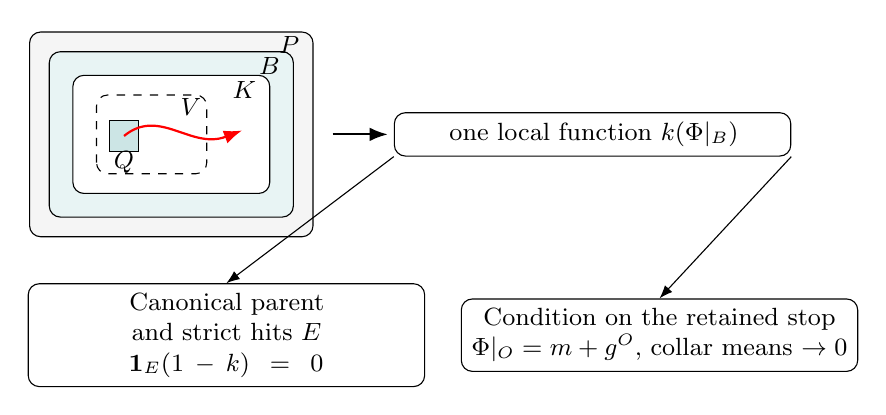
\begin{tikzpicture}[font=\small,>=Latex]
 \draw[rounded corners,fill=gray!8] (0,0) rectangle (3.6,2.6);
 \draw[rounded corners,fill=teal!9] (.25,.25) rectangle (3.35,2.35);
 \draw[rounded corners,fill=white] (.55,.55) rectangle (3.05,2.05);
 \draw[dashed,rounded corners] (.85,.8) rectangle (2.25,1.8);
 \draw[fill=teal!20] (1.02,1.08) rectangle (1.38,1.48);
 \draw[thick,red,->] (1.2,1.28) .. controls (1.65,1.65) and (2.05,1.1) .. (2.7,1.35);
 \node at (1.2,.94) {\(Q\)};
 \node at (2.05,1.65) {\(V\)};
 \node[anchor=east] at (3.0,1.87) {\(K\)};
 \node[anchor=east] at (3.3,2.17) {\(B\)};
 \node[anchor=east] at (3.55,2.43) {\(P\)};
 \draw[->,thick] (3.85,1.3)--(4.55,1.3);
 \node[draw,rounded corners,align=center,text width=4.8cm] (ker) at (7.15,1.3)
   {one local function \(k(\Phi|_B)\)};
 \node[draw,rounded corners,align=center,text width=4.8cm] (force) at (2.5,-1.25)
   {Canonical parent and strict hits \(E\)\\\(\ind_E(1-k)=0\)};
 \node[draw,rounded corners,align=center,text width=4.8cm] (bound) at (8,-1.25)
   {Condition on the retained stop\\\(\Phi|_O=m+g^O\), collar means \(\to0\)};
 \draw[->] (ker.south west)--(force.north);
 \draw[->] (ker.south east)--(bound.north);
\end{tikzpicture}
\caption{The path test crosses \(V\) inside \(K\), and the separated
buffers \(B\) and \(P\) make its kernel common to different Gaussian
domains. Calibration in the canonical parent gives an identity on the
field space. The upper bound uses the conditional GFF law of the stopped
component.}
\label{fig:kernel-conditioning}
\end{figure}

\subsection{The zero-boundary collar bound}

Fix a bounded simply connected \(O\), a compact rational polygon
\(Q\Subset O\), and a regular inner exhaustion
\(Q\Subset O_1\Subset O_2\Subset\cdots\uparrow O\).
For the \(j\)-th collar take
\[
       V=O_j,\qquad K=O_{j+2},\qquad B=O_{j+3},\qquad P=O_{j+4}.
\]
Use regular inner cable approximations of \(O\) on the common grid.
They have complement-Hausdorff convergence, uniformly bounded
connectivity, and contain every fixed \(\mathsf P_n\) for fine mesh.
Write \(T_{j,n}^{\pm}\) for the zero-threshold tests. We claim
\begin{equation}
       \lim_{j\to\infty}\limsup_{n\to\infty}
                 \P(T_{j,n}^{\pm}=1)=0.
 \label{eq:zero-boundary-collar}
\end{equation}

A one-sign path in an interior buffer is contained in the closure of
one cable sign component. Interior vertex values are almost surely
nonzero. On an edge, the nonnegative or nonpositive intervals are
closures of Brownian excursions; allowing their zero endpoints does
not join distinct interior sign components. Thus a crossing component
has a fixed positive lower diameter once the collar is sufficiently
far from \(Q\).

We make the rank and limit order explicit. Let
\(\mathcal C_{r,n}\) be the cable excursion supports in decreasing
diameter order, with the ranking convention of \cite{ALS2023}, and
let \(\mathcal C_r\) be their continuum limits. Theorems 3 and 28
of that paper give joint Hausdorff convergence for every fixed finite
list of ranks. Theorem 1 gives finitely many positive-diameter supports
above any fixed size, and its CLE/FPS construction in Section 3 places
each support compactly inside \(O\). These facts hold for the rough
simply connected \(O\) and the regular complement-Hausdorff
approximations just chosen.

Fix \(j_0\) and slightly enlarge \(Q\) within \(O_{j_0}\). Let
\(d>0\) be the distance of this enlargement from
\(O\setminus O_{j_0}\). For \(j\ge j_0\) and fine mesh, every crossing
component has diameter at least \(d\). If one has rank larger than \(N\),
then \(\diam\mathcal C_{N+1,n}\ge d\). Fixed-rank convergence gives
\[
 \limsup_{n\to\infty}
 \P(\text{a crossing component has rank}>N)
 \le \P(\diam\mathcal C_{N+1}\ge d/2).
\]
The right side tends to zero as \(N\to\infty\) by positive-diameter
finiteness. For the first \(N\) limiting supports, compact containment
implies that all lie in \(O_{j-1}\) with probability tending to one as
\(j\to\infty\). At fixed \(j\), their Hausdorff convergence then puts
the first \(N\) approximants inside \(O_j\), since
\(\overline O_{j-1}\Subset O_j\). Consequently
\[
 \limsup_{j\to\infty}\limsup_{n\to\infty}
       \P(T_{j,n}^{\pm}=1)
 \le \P(\diam\mathcal C_{N+1}\ge d/2).
\]
Send \(N\to\infty\). This proves \eqref{eq:zero-boundary-collar}:
the mesh limit is first for each fixed collar, the collar moves next,
and the finite rank truncation is removed last.

Let \(k_{j,0}^{\pm}\) be the common kernels selected for these
countably many collar choices. For fixed \(j\), the mixed-expectation
conclusion of \cref{lem:local-kernel} in \(O\) identifies its integral
with the mesh limit of the bounded test. Thus
\begin{equation}
       \lim_{j\to\infty}
       \E[k_{j,0}^{\pm}(g^O|_{B_j})]=0,
       \qquad g^O\text{ a zero-boundary GFF in }O.
 \label{eq:zero-boundary-kernel}
\end{equation}
This proof applies directly to rough \(O\). The total variation statement
in \cref{lem:kernel-exhaustion} concerns a fixed buffer and supplies no
estimate with a collar moving toward the boundary.

\subsection{No crossing of a stopped component}

\begin{proposition}[No crossing]
\label{prop:no-crossing}
Let \(O\) be a component of a stopped exploration from
\cref{prop:exploration-thin}, with retained sigma-field \(\mathscr E\).
Suppose \(O\) lies in an initial free parent \(P_0\) of label \(b_0\in a\Z\), or in
one pointed wired parent \(P_0\) of label \(b_0=\pm a\). As provided there,
\(O\) is simply connected and, conditionally on \(\mathscr E\),
\[
              h|_O=m+g^O,\qquad m-b_0\in2a\Z.
\]
No canonical free cluster descended from that parent meets both \(O\)
and \(\partial O\). The conclusion holds simultaneously for all
pointed components and all recursive generations, and after a restart
in a captured odd layer with its new incoming label.

In the wired case \(O\) may be a residual component of the global
composite exploration of the original \(h\). The proof uses
\(O\subset P_0\), simple connectedness, and the
displayed conditional law. It requires no connectedness of the
explored set relative to that parent and no separately selected
lattice sweep inside a limiting wired hole.
\end{proposition}

\begin{proof}
First work in an indexed canonical parent \(D_{\mathrm{par}}\) whose
total field is \(b+f\).
For a positive first-generation cluster \(C\),
\cref{lem:canonical-geometry} supplies a containing positive excursion
at total level \(b\) and a containing upper FPS with sublevel paths at
total level \(b+2a\). For a negative cluster the containing paths are
below \(b\) and above \(b-2a\). The parent is the initial domain or a
canonical Jordan hole; its regular auxiliary approximations satisfy
the coupled convergence hypotheses used above.

Suppose \(C\) meets both \(O\) and \(\partial O\), and choose a rational
\(Q\Subset O\) whose interior it meets. In a regular inner exhaustion
as above, connectedness of \(C\) makes it meet \(\partial O_{j+1}\)
for every large \(j\). This gives the two strict neighborhoods for the
excursion test: the second lies in
\(O_{j+2}\setminus\overline O_j\). The FPS test needs only the strict
inner hit, because its boundary-connected path must exit the fixed
collar. On the relevant-parent event \(O\subset D_{\mathrm{par}}\),
all buffers are contained in this canonical parent.

The stopped label and this parent label belong to the same affine
lattice \(b_0+2a\Z\). For a positive cluster, either \(m\le b\), so
the excursion forces the above-\(m\) test, or \(m\ge b+2a\), so the
upper FPS forces the below-\(m\) test. For a negative cluster, either
\(m\ge b\), using the below-\(m\) excursion, or \(m\le b-2a\), using
the above-\(m\) FPS. These alternatives exhaust the lattice. The
absolute threshold \(m\) belongs to \(a\Z\).

Calibrate both tests at every fixed threshold in \(a\Z\) in the
canonical parent, conditional on its ancestor data. For the excursion,
use the forcing identity for each fixed containing rank and take their
countable union; for the FPS use the whole-set identity. The path
implications and \eqref{eq:kernel-forcing} then hold simultaneously
for the countable choices of parent index, rank, threshold, and collar.
They are identities on the original field space and survive adjoining
the stop. To state the bound globally, fix an indexed candidate \(C\)
and a rational \(Q\), and select the collar from the stopped state by
the rule described below. Let \(\mathsf H_j\in\mathscr E\) record that
the selected pointed component and its \(j\)th collar are defined with
the required clearances inside \(O\). Let \(\mathsf L_j\) record that
the indexed candidate and its parent \(D_{\mathrm{par}}\) exist and that
\(\overline P_j\subset D_{\mathrm{par}}\). This latter event may depend
on canonical data. Declare it false when \(\mathsf H_j\) fails, use the
empty set for an absent candidate or component, and put
\[
 \mathsf C_Q=\{C\cap\operatorname{int}Q\ne\varnothing,\,
                     C\cap\partial O\ne\varnothing\}.
\]
The right side below is defined to be zero outside \(\mathsf H_j\).
Substituting the stopped-measurable \(m\) in the simultaneous forcing
identities gives the global pointwise bound
\begin{equation}
 \ind_{\mathsf H_j\cap\mathsf L_j\cap\mathsf C_Q}
 \le \ind_{\mathsf H_j}
       \bigl(k_{j,m}^{+}(h|_{B_j})+k_{j,m}^{-}(h|_{B_j})\bigr).
 \label{eq:crossing-kernel-bound}
\end{equation}
The direction selected by the unknown parent label \(b\) has disappeared
from this inequality. In particular \(b\) need not be measurable in
\(\mathscr E\).

Condition now only on \(\mathscr E\). The event \(\mathsf H_j\), the
collar, and \(m\) are stopped-measurable. The component law gives
\begin{align*}
 \Pr(\mathsf H_j\cap\mathsf L_j\cap\mathsf C_Q\mid\mathscr E)
 &\le \ind_{\mathsf H_j}\E\!\left[
   k_{j,m}^{+}(m+g^O|_{B_j})+
   k_{j,m}^{-}(m+g^O|_{B_j})\,\middle|\,\mathscr E\right]
 \\&=
 \ind_{\mathsf H_j}\E\!\left[
   k_{j,0}^{+}(g^O|_{B_j})+
   k_{j,0}^{-}(g^O|_{B_j})\,\middle|\,\mathscr E\right],
\end{align*}
where \eqref{eq:kernel-threshold} is applied under that conditional
Gaussian law. For each realized \(O\), \eqref{eq:zero-boundary-kernel}
makes the right side tend to zero as \(j\to\infty\). On the branch where
this parent is relevant, a crossing with witness \(Q\) belongs to
\(\mathsf H_j\cap\mathsf L_j\) for every sufficiently large \(j\).
Conditional Fatou applied to the left indicators therefore gives zero
conditional probability for that relevant crossing. No conditioning
on \(\mathsf L_j\) is used.

All random choices can be made within the countable families already
selected. An open hit has a rational polygon \(Q\) as witness. The
closed-set coordinate of the stop determines whether a rational polygon
has positive clearance inside \(O\). Choose successively the first
regular rational polygon containing the preceding one and the next
finite list of rational compact buffers. Simple connectedness ensures
such a nested exhaustion exists, and the clearance tests make the choice
\(\mathscr E\)-measurable. Partition by each finite collar and threshold
choice before conditioning. The random-domain clause of
\cref{lem:local-kernel} and bounded convergence justify the displayed
conditional integrals. There are countably many components and
canonical clusters.

It remains to justify that the same argument reaches every recursive
parent. Assume it for the ancestors of a candidate cluster. If an
ancestor lies wholly in \(O\), its filled disk lies in \(O\): its
outer Jordan loop is inside the simply connected \(O\), so the
connected complement of \(O\) cannot enter that loop without crossing
it. All descendants then stay in \(O\). Otherwise, an ancestor that
does not cross \(O\) and does not lie inside it is disjoint from \(O\).
Connectedness puts \(O\) in one complementary canonical hole, unless
the candidate descendant is outside \(O\) already. In the relevant
hole the incoming label is some \(b\in b_0+2a\Z\). The same absolute
threshold argument applies there. On this branch \(O\subset D_{\mathrm{par}}\),
so \(\mathsf L_j\) holds for every sufficiently large collar and the
global bound applies. Calibration conditions on that
parent's canonical data, while the upper bound continues to condition
only on the original retained stop. Induction proves the claim.

For a global composite wired stop, \(A\) contains the wired layer, so
\(O\) lies in one pointed wired hole. Its label satisfies
\(m-b_0\in2a\Z\) with \(b_0=\pm a\), and all canonical descendants
have baselines in the same affine lattice. The preceding proof applies
in the original field using those absolute labels. No further
exploration is introduced inside the selected limiting hole.
\end{proof}

\section{Identification of the complete cluster collections}
\label{sec:identification}

The stopped carpets determine the odd holes and their relative height
jumps. They do not determine which holes belong to one current cluster.
We identify that partition first. Finite families of visible holes then
transfer the lattice count bounds to all generations of the canonical
construction. The remaining task is to recover every point of a cluster,
including points that are not detected by an odd hole.

\subsection{Marked odd holes and their supplying clusters}

Fix a countable dense set \(\mathcal Q\subset D\). For each \(q\in\mathcal Q\)
choose a nearest lattice representative on the relevant \(W\) lattice,
using one deterministic rule to break ties. We record odd holes by a
family label \(\iota\in\{\mathrm f,\mathrm w\}\), a mark \(q\), and an
odd depth \(r\geq1\). The label \(\mathrm f\) refers to the original free
dual current; \(\mathrm w\) refers only to the free primal descendants
after the wired boundary cluster has been exposed.

At depth zero, \(V_{\delta,0}^{\mathrm f}(q)\) is the original free
chamber, with wall value \(b_{\delta,0}^{\mathrm f}(q)=0\).
For \(\iota=\mathrm w\), it is the component face left by the wired
layer that contains the representative of \(q\), with its observed
value \(b_{\delta,0}^{\mathrm w}(q)\in\{-a,a\}\).
Given a valid \(V_{\delta,r-1}^{\iota}(q)\), expose its first odd
carpet and let \(V_{\delta,r}^{\iota}(q)\) be the unsearched hole
containing the representative, with observed wall value
\(b_{\delta,r}^{\iota}(q)\). Write \(C_{\delta,r}^{\iota}(q)\)
for the current cluster supplying that odd rim, and put
\[
 \epsilon_{\delta,r}^{\iota}(q)
   =\frac{b_{\delta,r}^{\iota}(q)
               -b_{\delta,r-1}^{\iota}(q)}{2a}\in\{-1,1\}.
\]
If the representative is outside the chamber, lies on the revealed
carpet, or no such hole remains, give this observation and all its
descendants the cemetery value \(\dagger\), and set its sign to zero.
Validity, odd depth, and the supplying cluster depend only on the
unsigned data \((N,s)\), not on the free transverse colors \(d\).

The continuum observations \(V_r^\iota(q)\), \(b_r^\iota(q)\), and
\(\epsilon_r^\iota(q)\) are defined in the same way from the canonical
odd carpets of \cref{lem:canonical-geometry}. At depth zero the free
parent is \(D\), while the wired parent is the component of
\(D\setminus C_\partial\) containing \(q\), with its label \(\pm a\).
Use the same cemetery convention if a mark lies on a continuum carpet.
For a valid observation, \(C_r^\iota(q)\) denotes the retained canonical
cluster whose odd hole is \(V_r^\iota(q)\). The one-arm estimates in
the proof of \cref{lem:cut-neighborhoods} make every fixed mark miss
the limiting carpets almost surely. Every canonical odd hole contains a mark, so
these countably many observations see all odd holes at every finite
depth.

Here and below convergence of a marked hole is \emph{pointed}:
the closed carpet and its complement determine the limiting component
containing the mark, and every compact subset of that component is
eventually inside the discrete component. We do not assert Hausdorff
convergence of the closures of individual holes. In particular, one
discrete component may split into several pointed limiting components.

Abbreviate an address \((\iota,q,r)\) by \(i\), and write \(V_\delta(i)\),
\(C_\delta(i)\), and \(\epsilon_\delta(i)\), with the analogous notation
in the limit. For two addresses in the same family, define
\(i\sim_\delta j\) when both are valid and
\(C_\delta(i)=C_\delta(j)\); otherwise the relation is false.
Define \(i\sim j\) by the same rule for the supplying canonical
clusters, with a false relation whenever either address is invalid.

Fix any mesh subsequence. The whole-domain bound
\cref{cor:global-cluster-counts} and \cref{lem:matching-topology}
give compact containment of the two encoded collection factors
\(F(\cC_\delta^{\rm f})\) and \(F(\cC_\delta^{\rm w})\) in the
locally finite part of \(\mathfrak X\), the compact hyperspace over
the fixed enclosing square \(X\).
The height is tight by \cref{thm:flat-gff}. We pass to a joint further
subsequence retaining the closed carpets, their marked pointed
components and labels, the marked supplier supports in
\(\mathscr H\cup\{\dagger\}\) with an isolated cemetery value, and
the bits \(i\sim_\delta j\) for every fixed pair of addresses.
These supplier coordinates are compact;
they are separate from the contributor lists introduced later.
Write \(F_*^\iota\) for the locally finite outer Hausdorff limits of
the encoded collections. The relation coordinates are finite-valued;
on a joint representation they are eventually constant, with limiting
relation denoted by \(\sim_*\). This retains the finite identity
relations needed below, not numerical cluster identifiers across meshes.
By \cref{prop:stopped-tvs} and the one-arm estimate, for every finite
family of addresses the validity indicators and the signs in
\(\{-1,0,1\}\) converge jointly to their canonical counterparts.
In particular all bounded products of these signs converge in
expectation.

The use of \(X\) is necessary because an admissible polygon may
protrude outside \(D\). For each compact set disjoint from \(\partial D\),
uniform convergence of the boundary parametrizations preserves its
winding number for all sufficiently small mesh. Hence the polygonal
closures eventually lie in every fixed neighborhood of \(\overline D\),
and every Hausdorff limit of lattice supports lies in \(\overline D\).

We will use one elementary property of pointed convergence. If a sealed
discrete hole has pointed limit \(V\), every point of \(\partial V\)
is approached by its sealing boundary. Otherwise a ball around such a
point would avoid the discrete boundaries along a subsequence. Since
it meets a compact subset of \(V\), that connected ball would then lie
in the discrete hole, enlarging its pointed limit across the boundary.
The sealing boundary lies within \(O(\delta)\) of its supplying current
cluster. Consequently any Hausdorff limit of those suppliers contains
\(\partial V\); if the supplier has been revealed at a stop, the limiting
explored set contains \(\partial V\) as well.

\begin{lemma}[The restricted field determines its flat label]
\label{lem:recover-flat-label}
Let \(O\) be a random bounded simply connected domain with a marked
point \(q\in O\), and let \(f\) be a distribution on \(O\).
Suppose \(O,q,m\) are measurable in a sigma-field \(\mathcal E\) and,
conditionally on \(\mathcal E\), one has \(f=m+h^O\), where \(m\in\R\)
and \(h^O\) is a zero-boundary GFF. There is a measurable function of
\((O,q,f)\) alone that equals \(m\) almost surely. Thus two such conditional descriptions
of the same pointed domain and restricted field have the same label.
\end{lemma}

\begin{proof}
Let \(\phi_O:\mathbb D\to O\) be normalized by
\(\phi_O(0)=q\) and \(\phi'_O(0)>0\). Rational polygonal inner
exhaustions, normal-family compactness, and uniqueness of the normalized
limit make \(\phi_O\) measurable in \((O,q)\).
Push uniform angular probability measure \(\dd\vartheta/(2\pi)\) on
\(|z|=r\) forward by \(\phi_O\). Conformal invariance of the Green
kernel gives covariance \(-\log\max(r,s)\) for the zero-boundary
averages at radii \(r,s\). The radius-\(r\) average of \(f\) thus has
mean \(m\) and variance \(-\log r\).

For \(r_j=1-2^{-j}\), approximate the angular measure by a smooth
radial probability test \(\nu_j\) compactly supported in the disk,
with squared Green-energy error at most \(2^{-j}\).
Such choices are deterministic: the covariance
\(-\log\max(r,s)\) is continuous near each positive \(r_j\), so
radial smoothing converges in energy. Push \(\nu_j\) forward by
\(\phi_O\) to obtain a smooth compactly supported test \(\psi_j(O,q)\).
This test is measurable in the pointed domain, and evaluation
\(f(\psi_j(O,q))\) is measurable in \((O,q,f)\). Its conditional
mean is \(m\), and its conditional variance is at most
\[
 2(-\log r_j)+2^{1-j}.
\]
The sum of these variances is finite. Chebyshev's inequality and
Borel--Cantelli therefore give \(f(\psi_j(O,q))\to m\) almost surely.
Define the function in the statement by this limit when it exists,
and by zero otherwise. The construction uses conformal maps only on
compact subsets of the disk, so no boundary extension of \(O\) is
needed. The conformal identities are recalled in
\cite[Chapter~6, Sections~1.1 and~5.2]{Ahlfors1979}.
\end{proof}

\begin{proposition}[The visible partition]
\label{prop:partition}
Almost surely, \(i\sim_*j\) if and only if \(i\sim j\), simultaneously
for every pair of marked addresses in either current family. Their
relative signs also agree. Each retained canonical cluster \(C\) has
a marked address \(i\) such that every Hausdorff limit of
\(C_\delta(i)\) contains \(C\). For every finite family of distinct
canonical clusters, their chosen supplying lattice clusters are
eventually distinct.
\end{proposition}

\begin{proof}
We first show \(i\sim j\Rightarrow i\sim_*j\). All odd holes of one
retained canonical cluster have the same odd depth \(r\) and the same
parent at depth \(r-1\): entering any odd hole increases the depth, and
later clusters lie inside it. Let \(V_1,V_2\) be two marked odd holes
of such a cluster \(C\), and suppose that their lattice suppliers are
distinct along the retained subsequence.
If \(V_1=V_2\), a compact path inside that hole already puts both
marks in the same discrete hole for all sufficiently small mesh.
We may therefore assume that \(V_1\) and \(V_2\) are distinct.

Use the following fixed connected search. Starting from the exterior,
repeatedly add the lexicographically first unvisited current-lattice
vertex adjacent in the underlying graph to the explored region, and
reveal its entire current cluster. For the wired family start from the
completely exposed wired layer; the same rule interleaves its residual
chambers. The explored union remains connected to the original boundary.
For the two fixed marks count the surrounding odd rims already revealed,
and stop when either counter first reaches \(r\). This rule uses only the
revealed history; it never asks for the identity of a future hole.
If neither counter reaches \(r\), give the stop a cemetery value;
on the event under consideration it is eventually active.
Adjoin the retained stopped states for all these countably many fixed
rules to the joint subsequence. By \cref{prop:exploration-thin}, each
has the stated component laws conditional on its own limiting stopped
state. The future supplier relation is not included in that state.

The two marks lie in one pointed parent at depth \(r-1\). A compact
path inside that parent joining them is eventually inside the same
discrete parent, by pointed convergence. This implication does not
assert the converse through a pinch. The exterior seed must cross
all of their shared enclosing odd rims before it can reach either
\(r\)th rim. Suppose the stop discovers the rim of \(V_1\) first.
The other mark has then seen exactly the common \(r-1\) odd jumps;
any intervening even holes contribute zero. Its stopped value is the
common parent label \(b\).

The newly revealed supplier and its sealing boundary put
\(\partial V_1\) in the limiting explored set \(A\). Hence \(C\)
meets \(A\). If a connected cluster meeting \(A\) entered any component
of the complement, it would also meet that component's boundary.
\Cref{prop:no-crossing}, applied at the appropriate canonical
generation and after subtracting the parent label, forbids this.
Therefore \(C\subset A\), in particular \(\partial V_2\subset A\).

The entire discrete interior of the second odd hole is still
unsearched. A seed vertex could enter it only after meeting its
enclosing supplier, which would have raised the second counter to
\(r\). A different current cluster inside that hole is trapped there
by the supplier and its sealing rim, so it could have been discovered
only from a seed vertex in the same interior. Thus the whole explored
set, not only the seed, misses the second discrete hole. Every compact
subset of \(V_2\), with a slightly larger compact neighborhood,
eventually lies in that untouched hole. It follows that \(A\) misses
\(V_2\). Since \(\partial V_2\subset A\), the domain \(V_2\) is
itself a stopped complementary component.

Its stopped conditional law has flat label \(b\). The labelled odd
carpet gives the same \(V_2\) the label \(b+2a\epsilon(i)\), which
differs from \(b\). Both are conditional descriptions of the same
restricted field on the same pointed domain, so
\cref{lem:recover-flat-label} makes this impossible. The conditional
laws were used at the fixed observable stop, not after conditioning
on the hypothesis of distinct suppliers. This proves the inclusion
at every finite odd depth, including clusters reached after any
number of even restarts.

\begin{figure}[t]
\centering
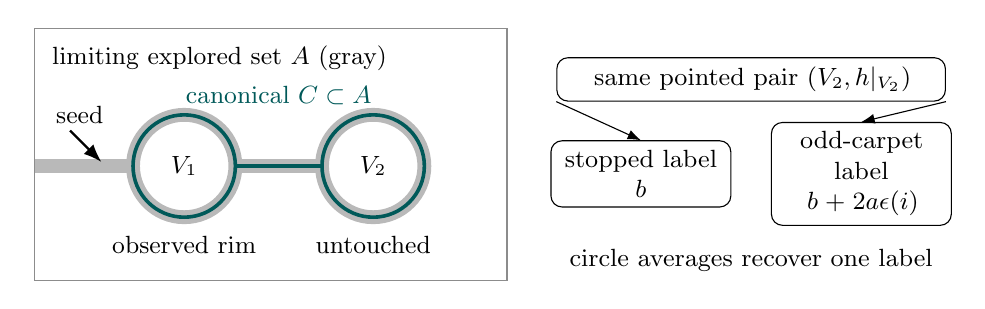
\begin{tikzpicture}[font=\small,>=Latex]
 \draw[black!45] (0,0) rectangle (6,3.2);
 \node[anchor=north west] at (.1,3.1) {limiting explored set \(A\) (gray)};
 \draw[gray!55,line width=5pt] (0,1.45)--(1.25,1.45);
 \draw[gray!55,line width=5pt] (1.9,1.45) circle (.65);
 \draw[gray!55,line width=5pt] (4.3,1.45) circle (.65);
 \draw[gray!55,line width=5pt] (2.55,1.45)--(3.65,1.45);
 \draw[teal!70!black,line width=1.3pt] (1.9,1.45) circle (.65);
 \draw[teal!70!black,line width=1.3pt] (4.3,1.45) circle (.65);
 \draw[teal!70!black,line width=1.3pt] (2.55,1.45)--(3.65,1.45);
 \draw[->,thick] (.45,1.9)--(.85,1.5);
 \node[anchor=west] at (.15,2.1) {seed};
 \node at (1.9,1.45) {\(V_1\)};
 \node at (1.9,.45) {observed rim};
 \node at (4.3,1.45) {\(V_2\)};
 \node at (4.3,.45) {untouched};
 \node[teal!70!black] at (3.1,2.35) {canonical \(C\subset A\)};
 \node[draw,rounded corners,align=center,text width=4.7cm]
   (same) at (9.1,2.55) {same pointed pair \((V_2,h|_{V_2})\)};
 \node[draw,rounded corners,align=center,text width=2.05cm]
   (stop) at (7.7,1.35) {stopped label\\\(b\)};
 \node[draw,rounded corners,align=center,text width=2.05cm]
   (carpet) at (10.5,1.35) {odd-carpet label\\\(b+2a\epsilon(i)\)};
 \draw[->] (same.south west)--(stop.north);
 \draw[->] (same.south east)--(carpet.north);
 \node[align=center,text width=5cm] at (9.1,.25)
   {circle averages recover one label};
\end{tikzpicture}
\caption{The hypothetical distinct-supplier case at the fixed marked
stop. The first rim puts \(\partial V_1\) in \(A\); no crossing then
puts the whole canonical cluster \(C\), including \(\partial V_2\),
in \(A\), while the discrete interior of \(V_2\) remains untouched.
Its two proposed labels contradict \cref{lem:recover-flat-label}.
The strokes depict inclusion and connectedness, not area or distances.}
\label{fig:visible-partition}
\end{figure}

To exclude extra identifications, use the relative signs. Conditional
on the unsigned lattice data \((N,s)\), the signs of different free
current clusters are independent and fair, and one cluster has the
same sign at all its odd holes. The validity of a marked address is
also unsigned. With our zero sign and false relation at \(\dagger\),
\cref{lem:finite-cuts} therefore gives, for every fixed pair of
addresses in the same current family,
\begin{equation}
 \E[\epsilon_\delta(i)\epsilon_\delta(j)]
       =\P(i\sim_\delta j).
 \label{eq:partition-sign-discrete}
\end{equation}
The canonical fair-sign statement in \cref{lem:canonical-geometry}
gives the same identity with \(\epsilon\) and \(\sim\) for each fixed
pair in that same family. Joint
labelled-carpet convergence passes the bounded sign product to the
limit, while the retained relation bits pass the right side to
\(\P(i\sim_*j)\). Hence
\[
 \P(i\sim_*j)=\E[\epsilon(i)\epsilon(j)]=\P(i\sim j).
\]
The inclusion already proved makes
\(\ind_{\{i\sim_*j\}}-\ind_{\{i\sim j\}}\) nonnegative. Its
expectation is zero, so it vanishes almost surely. This argument
uses global fixed addresses and does not require equality of
discrete parent components to be continuous through a pinch.
The countable intersection over all pairs proves the asserted
partition equality; the relative signs are already the limits
of the marked labels.

Finally choose, for each canonical cluster, one address \(i\)
supplying one of its odd holes. Every other marked odd hole of
that cluster has the same lattice supplier as \(i\) for all
sufficiently small mesh. The pointed-boundary observation above
therefore puts all its odd-hole boundaries in every Hausdorff
limit of \(C_\delta(i)\). Their union is dense in the canonical
cluster by \cref{lem:canonical-geometry}. This proves containment.
For finitely many distinct canonical clusters, the corresponding
relation bits are eventually false, so their suppliers are
eventually distinct.
\end{proof}

Fix an enumeration of the marked addresses. For each canonical cluster,
choose its first supplying address in this enumeration and call the
associated sequence \(C_\delta(i)\) its \emph{visible precursor}.
This is auxiliary information retained for the proof; the matching
topology itself forgets multiplicity.

\begin{corollary}[All-generation local finiteness]
\label{cor:canonical-local-finiteness}
Almost surely, the entire canonical free cluster family has only
finitely many members of diameter greater than any given
$\eps>0$. The same holds for the wired family, including all
descendants. These bounds are compatible with the uniform tight
macroscopic lattice counts.
\end{corollary}

\begin{proof}
Consider any finite family of $M$ canonical clusters of diameter
greater than $\eps$. In each cluster choose two points more than
$\eps$ apart. Density of
odd rims gives two nearly as separated rim points, witnessed by
finitely many nearby odd holes and dense interior test points.
The individual holes need not have diameter comparable to
$\eps$. By \cref{prop:partition}, the two witnesses in each
cluster have one precursor, and the $M$ precursors are distinct.
For sufficiently small mesh each has diameter greater than
$\eps/2$. This finite choice involves only finitely many odd
depths and marks.

Thus, on the joint representation, the event of at least $M$
canonical clusters of diameter greater than $\eps$ implies at
least $M$ lattice clusters of diameter greater than $\eps/2$
eventually. Finite choices from the countable canonical family
and the dense test list suffice; no measurable choice from an
uncountable family is needed. Fatou's lemma and
\cref{cor:global-cluster-counts} make the probability of this event
tend to zero as $M\to\infty$. Countably many rational $\eps$
give the result. The same finite-witness argument can be performed
in the wired descendants, with the boundary cluster counted once.
This proof does not assume nested all-generation local finiteness
in advance.
\end{proof}

\subsection{A flat region cannot contain a revealed crossing}

We give the analytic observation that detects cluster pieces with
no visible jump. It concerns a distributional conditional mean,
not merely a harmonic function on the open complement.

\begin{lemma}[Flat patches]
\label{lem:flat-patch}
Let $h$ be a zero-boundary GFF in a bounded simply connected domain
$O$. Suppose an exploration with information $\cF_A$ describes a
boundary-connected closed set $A$ and a $\cF_A$-measurable distribution $h_A$ such that,
conditionally on $\cF_A$, the residual $h^A=h-h_A$ is the GFF on
$O\setminus A$ extended by zero through $A$, as a distribution on $O$.
The complementary components are assumed simply connected. Extra
randomness may be included in the exploration. For every
deterministic ball $B\Subset O$, almost surely on the event that
$h_A$ is one constant distribution throughout $B$, one has
$A\cap B=\varnothing$. If the conditional decomposition is given
only for tests supported in a neighborhood of $B$ and on a
$\cF_A$-measurable event $\Lambda$, the conclusion holds on $\Lambda$.
\end{lemma}

\begin{proof}
Fix a nonnegative smooth unit-mass mollifier $\rho$ supported in
the unit disk, and put $h_u=h*\rho_u$. For a nonnegative
$b\in C_c^\infty(B)$ set
\begin{equation}
 X_u=u^{-1}\int b(x)\exp(i\beta h_u(x))\,\dd x,
             \qquad \beta^2>2.
 \label{eq:flat-oscillatory}
\end{equation}
On the compact support of $b$, the normalized Green kernel gives
\[
 \E\exp\bigl(i\beta(h_u(x)-h_u(y))\bigr)
 \leq C\left(\frac{u}{|x-y|\vee u}\right)^{\beta^2}.
\]
Consequently
\begin{equation}
 \E|X_u|^2
 \leq C u^{-2}\int_0^{O(1)}
       \left(\frac{u}{r\vee u}\right)^{\beta^2}r\,\dd r
 \leq C.
 \label{eq:oscillatory-L2}
\end{equation}
For a smooth Gaussian exponential cylinder $Y=\exp(ih(\phi))$,
the Gaussian characteristic function and the bounds
$\Var(h_u(x))=\log(1/u)+O(1)$ and
$|\Cov(h_u(x),h(\phi))|\leq C_\phi$ imply
\[
 |\E[X_uY]|\leq C_\phi u^{\beta^2/2-1}\longrightarrow0.
\]
The linear span of these cylinders is dense in $L^2$ of the field.
Together with \eqref{eq:oscillatory-L2}, this proves
$X_u\rightharpoonup0$ weakly in $L^2$. It also proves weak
convergence on the full probability space with extra randomness:
replace any $L^2$ test variable by its conditional expectation
given $h$.

We next bound the conditional \emph{mollified} variance near $A$.
Let $U$ be a simply connected component of $O\setminus A$ and
write $r=|f^{-1}(w)|$, where $f:\mathbb D\to U$ maps zero to $z$.
The conformal Green formula and the growth and quarter estimates
proved or cited in \cref{sec:conformal-growth} give
\[
 G_U(z,w)=-\log r,
 \qquad |z-w|\leq\operatorname{cr}_U(z)\frac{r}{(1-r)^2}.
\]
For $r\geq1/2$ the Green function is at most $\log2$; for
$r<1/2$ the second inequality gives
\[
 G_U(z,w)\leq\log2+
       \log^+\frac{4\operatorname{cr}_U(z)}{|z-w|}.
\]
Koebe's quarter theorem gives
$\operatorname{cr}_U(z)\leq4\dist(z,\partial U)$. If
$\dist(x,A)\leq u$ and $z$ belongs to the mollifier at $x$, then
$\dist(z,\partial U)\leq2u$. Different components have zero
covariance, so the killed Green kernel satisfies on the mollifier
supports
\begin{equation}
 G_{O\setminus A}(z,w)
       \leq\log2+\log^+\frac{32u}{|z-w|}.
 \label{eq:cut-green-bound}
\end{equation}
Rescaling $z=x+u\zeta$, $w=x+u\omega$ and integrating the
locally integrable logarithm against the two mollifiers yields
\begin{equation}
 \Var(h_u^A(x)\mid\cF_A)\leq C_\rho
       \quad\text{if }\dist(x,A)\leq u.
 \label{eq:cut-mollified-variance}
\end{equation}
This is uniform in the exploration. It does not assert a finite
pointwise variance for the GFF itself.

Choose $B_0\Subset B_1\Subset B$ and take $b=1$ on $B_1$.
Let $E$ be the event that $h_A=m$ throughout $B$ and
$A\cap\overline B_0\ne\varnothing$. This is an exploration-
measurable event: obtain $m$ by testing against one fixed smooth
unit-mass function, and check equality of distributions on a
countable dense test family. In the localized version replace $E$
by $E\cap\Lambda$. On $E$, for small $u$,
\begin{equation}
 e^{-i\beta m}\E[X_u\mid\cF_A]
   =u^{-1}\int b(x)
      \exp\left(-\frac{\beta^2}{2}
          \Var(h_u^A(x)\mid\cF_A)\right)\,\dd x.
 \label{eq:flat-positive-integrand}
\end{equation}
All integrands are nonnegative. Since $A$ is connected to
$\partial O$ and meets $B_0$, its $u$-neighborhood in $B_1$ has
area at least $cu$, with deterministic $c>0$. To verify this
without assuming path connectedness, use the distance from a
point in $A\cap\overline B_0$: its image on the connected set
$A\cup\partial O$ is an interval. Choose points at radial spacings
$3u$ up to a fixed positive radius small enough that they lie in $B_1$.
Since $B_1\Subset O$, these points cannot lie on $\partial O$ and
therefore belong to $A$. Their disks of radius $u/2$ are
disjoint, lie in $B_1$, and are within distance $u$ of $A$.
There are at least $c/u$ of them.

Using \eqref{eq:cut-mollified-variance} in
\eqref{eq:flat-positive-integrand} therefore gives
\[
 \E[\ind_E e^{-i\beta m}X_u]\geq c'\P(E).
\]
The left side tends to zero by weak $L^2$ convergence, since
$\ind_Ee^{-i\beta m}$ is a fixed bounded random variable.
Thus $\P(E)=0$. A countable exhaustion of $B$ proves the lemma.
For a random initial component one first conditions on it and
subtracts its initial constant, then uses rational balls with
positive clearance. The conclusion is still a probability-zero
statement, so no bound uniform over all such domains is needed.
\end{proof}

\subsection{Open hole witnesses and the discovered mean}

A cluster with no limiting odd hole might still have many small discrete
holes. The next observation shows that those holes cannot retain positive
area away from the limiting cluster.

\begin{lemma}[Open witnesses for hole contributions]
\label{lem:hole-witnesses}
Let \(O\) be open. Suppose compact sets \(C_n\subset X\) converge in
Hausdorff distance to \(C\), and \(C\cap O\) has zero area. Let
\(U_n\subset O\) be open, with actual relative topological boundary
contained in \(C_n^{\eta_n}\), where \(\eta_n\to0\).
If the indicators of \(U_n\) converge on a dense subset of
\(O\setminus C\) to those of a union \(U\) of components of
\(O\setminus C\), then
\[
 \ind_{U_n}\longrightarrow\ind_U\quad\text{in }L^1_{\rm loc}(O).
\]
In particular, if every nonempty pointed open witness is absent,
the area of \(U_n\) on each compact subset of \(O\) tends to zero.
\end{lemma}

\begin{proof}
For \(x\notin C\), choose a small ball \(B_x\Subset O\setminus C\).
Its closure misses \(C_n^{\eta_n}\) for all large \(n\). Membership
in \(U_n\) is then constant throughout \(B_x\); otherwise the connected
ball would meet its actual relative boundary. A dense test point in
\(B_x\) determines this constant eventually. The indicator of \(U\)
is also constant there, since \(B_x\) lies in one component of
\(O\setminus C\). Thus the indicators converge at every point outside
\(C\). Dominated convergence and the zero area of \(C\) prove the claim.
\end{proof}

We now specify the sweeps used for complete support identification.
They are performed for each current family; the family label is
suppressed in the sweep notation.
For \(e\in\{\pm e_1,\pm e_2\}\), visit current-lattice vertices in
increasing order of \(e\cdot v\), completing every earlier lattice
column before beginning the next one. Within a column use a fixed
lexicographic order. The virtual exterior of the free graph is the
initial connected attachment. In the wired case first reveal the
boundary cluster completely and use it, together with the exterior,
as the attachment for all residual free chambers. When a vertex is
visited, add the edge to its neighbor in the preceding column and
reveal its entire current cluster. That neighbor has already been
visited or belongs to the initial filled region; it is never an
unsearched vertex farther ahead. The seed edges need not be current
edges. Thus the initial region, the added seed, and all revealed
clusters stay connected to the original boundary, and the exact cuts
in \cref{lem:finite-cuts} apply throughout.

We use two countable families of observable stops. A \emph{column stop}
ends after all vertices with \(e\cdot v\leq t\) have been visited, for
a rational \(t\). For rational \(b>0\), a \emph{recorded stop} ends just
after the \(k\)th newly discovered free cluster of diameter at least
\(b\), for a fixed \(k\geq1\). If that discovery never occurs, give
the stop a cemetery value. The rank \(k\) counts only these recorded
discoveries; arbitrarily many smaller clusters may precede them and
remain part of the explored set.

Write \(W_{0,\delta}\) for the initial revealed region: the boundary
perimeter in the free case and the wired current support in the wired
case. Its limit is respectively \(W_0=\partial D\) or
\(W_0=C_\partial\). Write \(S_\delta\) for the added moving seed and
\(A_{\delta,\tau}\) for the full explored set at a fixed stop \(\tau\).
For the wired family this is one composite exploration of the original
field, across all initial chambers. It does not choose a new lattice
exploration from a limiting hole that might have separated from a
shared discrete precursor.

Fix rational compact rectangles
\(Q\subset\operatorname{int}Q^+\Subset D\) and a rational \(r>0\).
On the event
\[
 \dist(Q^+,W_{0,\delta}\cup S_\delta)\geq r,
\]
call a discovered free cluster a \emph{contributor to \(Q^+\)} if
its support meets \(Q^+\) or its union \(\mathcal O_\delta(C)\) of
odd component faces meets \(Q^+\). List these clusters in their
relative discovery order, as
\(C_{\delta,1},\ldots,C_{\delta,L_\delta}\).
A listed cluster contains a seed contact. If its support meets \(Q^+\),
it has diameter at least \(r-O(\delta)\). If an odd hole meets \(Q^+\),
choose a point of that hole there. The cluster surrounds that point
and contains a seed contact at distance at least \(r\).
A point in a bounded complementary component lies in the convex hull
of the surrounding compact set, so the latter's diameter is at least
that distance, again up to the lattice boundary convention.
Therefore, for all sufficiently fine meshes,
\begin{equation}
 L_\delta\leq N_{\delta,0}(r/3),
 \label{eq:contributor-domination}
\end{equation}
where \(N_{\delta,0}(b)=\mathcal N_{\delta,\mathrm{initial}}(b)\)
counts all free clusters of diameter at least \(b\) in the initial
chamber family, as in \cref{eq:spatial-contributor-domination}.
\Cref{cor:global-cluster-counts} gives a uniform tail for this right
side conditional on the initial cut data. This is a pathwise bound
valid at every observable stop; it is not a tail bound after fixing
the completed history at that stop.

For these countably many fixed stops, retain the stopped states of
\cref{prop:exploration-thin}. For each fixed choice of sweep, stop,
\(Q,Q^+\), and \(r\), retain also the active clearance flag and,
when active, the integer \(L_\delta\),
the ordered supports, their relative signs, and the membership bits
of their odd-hole unions at all dense marks. Give the list a
cemetery value when inactive. The integer is tight by
\cref{eq:contributor-domination}, and a fixed-length list has compact
support coordinates in \(\mathscr H\). A further diagonal extraction
therefore makes \(L_\delta\) eventually equal to a finite \(L\) on
the joint representation, with limits \(C_{*,1},\ldots,C_{*,L}\).
The order is reindexed by \(1,\ldots,L_\delta\); raw discovery indices
are not asserted to be tight. Retain also, on the global representation,
the equality bits between each list entry and each marked supplier.
A missing list entry or invalid address has equality bit zero.
A list entry is \emph{visible} if it eventually equals a supplier at
some fixed valid marked address, and \emph{invisible} otherwise.
By \cref{prop:partition}, a visible entry has one associated canonical
cluster, denoted \(C_j^{\rm can}\).

We retain one further kind of auxiliary list on the global
representation. For each fixed \((e,b)\), let \(D_\delta(e,b)\) be
the number of recorded discoveries during the complete sweep, and
write their ordered supports as
\(\widehat C_{\delta,1}^{e,b},\ldots,
\widehat C_{\delta,D_\delta(e,b)}^{e,b}\).
The bound \(D_\delta(e,b)\leq N_{\delta,0}(b)\) makes the integer
length tight. A further diagonal extraction makes it eventually
equal to a finite \(D(e,b)\), and makes each recorded support converge
in \(\mathscr H\); missing ranks have the cemetery value. Retain also
the equality bits between every record and every marked supplier,
set to zero for a missing rank or invalid address.
They are eventually constant on the joint representation.
Call a stabilized record visible if one such bit is eventually one
for a fixed valid address, and invisible otherwise. These lists keep
their order and multiplicity even if several supports have the same
limit. Their lengths are auxiliary coordinates and are not identified
with counts obtained by cutting off the limiting encoded family at
diameter \(b\).

Only coordinates measurable at the fixed stop generate its limiting
sigma-field \(\mathscr E_\tau\): the explored set, seed, observed labels,
and discovered list data. The global representation also carries
future marked suppliers, complete recorded lists, and the canonical
field. They are not added to \(\mathscr E_\tau\) when applying the
stopped conditional laws. In later uses \(r\) is chosen below a
positive limiting clearance, so the discrete clearance flag is
eventually active.

\begin{proposition}[The discovered mean]
\label{prop:discovered-mean}
Let \(\tau\) be one of the fixed stopped sweeps above, with limiting
explored set \(A_\tau\), and write
\(M_\tau=\E[h\mid\mathscr E_\tau]\) as a distribution on tests.
On each connected compact localization \(Q\subset\operatorname{int}Q^+\)
above at positive distance from \(W_0\) and the moving seed,
\(M_\tau\) is the finite signed sum
\begin{equation}
 M_\tau=b_0+2a\sum_{\substack{j\text{ visible}\\
                       \text{in the localized list}}}
       \epsilon_j\ind_{\mathcal O(C_j^{\rm can})}.
 \label{eq:canonical-discovered-mean}
\end{equation}
Here \(b_0=0\) for the original free family. For the wired composite
exploration, \(b_0\in\{-a,a\}\) is the label of the initial pointed
wired hole containing the region. The sum is finite on each such
localization because its contributor list is finite. An invisible
entry has zero contribution. Consequently \(M_\tau\) is a constant
distribution on every ball missing \(W_0\), the moving seed, and the
canonical supports associated with its local contributors.
\end{proposition}

\begin{proof}
Work first with \(Q\subset\operatorname{int}Q^+\) and a positive
clearance as above, on an outcome where the list length has stabilized.
Every \(C_{*,j}\) is contained in \(A_\tau\). By
\cref{prop:exploration-thin}, it has zero area in
\(\operatorname{int}Q^+\), and the actual relative boundary of
\(\mathcal O_\delta(C_{\delta,j})\) lies within \(O(\delta)\) of
\(C_{\delta,j}\).

We identify membership at a dense mark \(q\in\mathcal Q\cap
(\operatorname{int}Q^+\setminus C_{*,j})\). If \(q\) belongs to the
odd-hole union along infinitely many meshes, its positive distance
from \(C_{*,j}\) gives a fixed disk about \(q\) inside that union
on those meshes. The relevant odd depth is bounded by \(L\).
Indeed every enclosing odd ancestor is a distinct cluster: after
entering its odd hole, later clusters lie strictly inside that hole.
The exterior-connected seed must discover each such ancestor before
\(C_{\delta,j}\), and its odd-hole union contains \(q\). It is
therefore another entry of the same list for \(Q^+\).
After passing to a further subsequence, the depth is one fixed
\(r\leq L\), and the representative of \(q\) lies in the fixed disk.
Thus \(C_{\delta,j}\) supplies the marked address
\((\iota,q,r)\). The stabilized equality bit makes the entry visible,
and \cref{prop:partition} identifies its canonical cluster and odd
hole.

Conversely, suppose the entry is visible and \(q\notin C_{*,j}\)
lies in an odd hole of \(C_j^{\rm can}\). That hole has the marked
address \((\iota,q,r)\) at a finite depth. The partition equality
makes its supplier equal to the list entry for all sufficiently
small mesh, so \(q\) eventually belongs to
\(\mathcal O_\delta(C_{\delta,j})\). These two implications show
that the membership indicators converge at every dense mark off
\(C_{*,j}\). In the visible case their limit is
\[
 \ind_{\mathcal O(C_j^{\rm can})\setminus C_{*,j}},
\]
and in the invisible case it is zero. This also rules out
oscillation between membership and nonmembership: any infinite
membership subsequence supplies a fixed visible address, after
which the converse gives eventual membership.

The displayed visible set is a union of components of
\(\operatorname{int}Q^+\setminus C_{*,j}\). In fact
\cref{prop:partition} gives \(C_j^{\rm can}\subset C_{*,j}\), and
the boundary of every canonical odd hole is contained in
\(C_j^{\rm can}\); a component of the smaller complement cannot
cross such a boundary. Removing \(C_{*,j}\) changes no area on this
region. We may therefore apply \cref{lem:hole-witnesses} to each
list entry. Its odd-hole indicators converge in \(L^1(Q)\) to the
canonical odd-hole indicator, or to zero for an invisible entry.
Thus even a collection of long or numerous collapsing holes has
vanishing area unless it supplies an open marked witness.

The signs have stabilized and the list is finite, so the discrete
signed sum in \cref{eq:discrete-discovered-mean} converges in
\(L^1(Q)\) to the sum in the statement. For a visible entry its sign
is the canonical sign because it eventually supplies a fixed marked
address. In the wired case the connected
rectangle \(Q^+\), being disjoint from \(W_0\), lies in one pointed
initial wired hole. Compact containment puts it in one discrete
initial hole for fine mesh, even if that hole pinches elsewhere.
Its initial label is therefore one constant \(b_0\in\{-a,a\}\)
on \(Q^+\). This supplies the additional baseline term.
Remove a deterministic truncation \(L\leq M\) using
\cref{eq:contributor-domination} and the initial count tail.
The uniform higher logarithmic moments in \cref{prop:log-moments}
give uniform integrability when passing tested conditional means.

Finally, \cref{prop:exploration-thin} identifies the full conditional
mean on these tests, including across \(A_\tau\), by its neighborhood
removal argument. Hence the ordinary function just obtained is
\(M_\tau\), with no extra distribution on the explored set.
On a connected ball avoiding \(C_j^{\rm can}\), its odd-hole indicator
is constant. The baseline is also constant on a ball avoiding \(W_0\).
The localized list contains only finitely many entries, regardless
of the diameters of their associated canonical clusters. This proves
the last assertion.
\end{proof}

\subsection{Complete matching, including invisible clusters}

\begin{proposition}[Matching of all positive-diameter clusters]
\label{prop:complete-matching}
Every positive-diameter Hausdorff limit of lattice free-current clusters
is one retained canonical cluster, and every retained canonical cluster
is the limit of its visible precursor. No distinct invisible precursor
has a positive-diameter limit. The same assertions hold for the free
primal descendants after the wired layer, jointly with that layer and
the height. Consequently
\[
 F_*^{\mathrm f}=F(\cC^{\rm f}),\qquad
 F_*^{\mathrm w}=F(\cC^{\rm w}),
\]
and both collections converge in the matching topology of
\cref{thm:main}.
\end{proposition}

\begin{proof}
\emph{Every point is on a canonical support or the initial wall.}
Let \(C_\delta\) be lattice free clusters with a positive-diameter
Hausdorff limit \(C_*\). The limit is compact and connected.
Take \(x\in C_*\setminus W_0\) and a distinct point \(y\in C_*\).
Choose an axial direction \(e\) and a rational \(t\) with
\(e\cdot y<t<e\cdot x\). At the fixed column stop \(\tau(e,t)\),
the cluster \(C_\delta\) has been discovered for all sufficiently
small mesh, because it has a point near \(y\) in an earlier column.
A small rational ball about \(x\) lies ahead of the seed and has
positive clearance from \(W_0\). The same clearances hold at fine mesh.
Choose \(Q\subset\operatorname{int}Q^+\) around that ball and a rational
lower clearance \(r\). The target cluster is an entry in the finite
localized list at this already specified stop.

Let \(\mathcal U_\tau\) be the finite union of the canonical supports
associated with that list's visible entries. If \(x\notin\mathcal U_\tau\),
a smaller rational ball \(B\) around \(x\) misses \(\mathcal U_\tau\),
\(W_0\), and the moving seed. By \cref{prop:discovered-mean},
\(M_\tau\) is a constant distribution on \(B\).
Let \(\Lambda_{Q^+}=\{\dist(Q^+,W_0\cup S)>0\}\), the
stopped-measurable clearance event for this localization. In the
present initial domains it is the event in
\cref{eq:stopped-full-characteristic}. That identity gives, for every
real smooth test \(\varphi\) supported in \(Q^+\),
\begin{equation}
 \ind_{\Lambda_{Q^+}}
 \E\!\left[e^{i(h-M_\tau)(\varphi)}\mid\mathscr E_\tau\right]
 =\ind_{\Lambda_{Q^+}}\exp\!\left\{-\tfrac12
       G_{D\setminus A_\tau}(\varphi,\varphi)\right\}.
 \label{eq:full-residual-use}
\end{equation}
It holds for all linear combinations of finitely many tests, with the
killed GFF extended by zero across \(A_\tau\). It therefore supplies
the local residual law required by \cref{lem:flat-patch}, including
the mollifiers whose supports cross the explored set. Since \(A_\tau\) is
boundary-connected and the complementary components are simply connected, that lemma
says \(A_\tau\cap B=\varnothing\). But \(C_\delta\) was revealed at
this stop, so \(C_*\subset A_\tau\), a contradiction.

The choice of \(B\) may depend on the later canonical data. Its
existence implies one of the countably many
\(\mathscr E_\tau\)-measurable zero events that \(M_\tau\) is constant
on a fixed rational ball and \(A_\tau\) meets it. The conditional law
used in each of these events is the one at the fixed stopped state.
All directions, column thresholds, balls, and localizations come from
countable families, and each localized list has finitely many entries.
The preceding conclusion therefore holds simultaneously for every
possible subsequential \(C_*\) and every \(x\in C_*\setminus W_0\).
We have proved
\begin{equation}
 C_*\subset W_0\ \cup\!\bigcup_{C\in\cC_{\rm can}}C,
 \label{eq:countable-cover}
\end{equation}
where \(\cC_{\rm can}\) is the complete canonical free family under
consideration. For wired descendants the argument used the single
composite exploration of the original \(h\). A ball away from \(W_0\)
lies in one pointed wired hole and has a constant initial label, even
when its discrete initial chamber pinches into several limiting holes.

The sets in the cover are compact and pairwise disjoint, including
\(W_0\): this follows from \cref{lem:canonical-geometry} and the fact
that each retained cluster lies strictly inside its parent. They form
a countable family. Their intersections with \(C_*\) are therefore
a disjoint closed cover of the compact connected set \(C_*\).
Sierpi\'nski's continuum partition theorem \cite{Sierpinski1918},
with a complete proof in \cite[Chapter~V, Theorem~5.10]{Freiwald2014},
says that at most one member of such a cover is nonempty.
Consequently \(C_*\) is contained in one canonical cluster or entirely
in \(W_0\).

We exclude the latter case using the actual chamber wall.
Let \(\Gamma_\delta\) be the component-side open \(W\) perimeter of
the initial chamber containing \(C_\delta\), with the medial resolution
at pinches. In the wired case \(W_{0,\delta}\) is a current support,
whereas the spatial estimate uses the attached matching wall.
\Cref{lem:chamber-rim-distance} gives
\[
 \sup_{z\in C_\delta}\dist(z,\Gamma_\delta)
 \leq \sup_{z\in C_\delta}\dist(z,W_{0,\delta})+O(\delta).
\]
Its first-exit proof uses the resolved chamber face: a segment from
an adjacent chamber point toward the revealed support first meets
this chamber's own medial rim, including at a pinch. The free case
uses the polygonal boundary.
If \(C_*\subset W_0\), Hausdorff convergence of \(C_\delta\) and
\(W_{0,\delta}\) makes the right side tend to zero.

Choose one fixed buffered square \(Q_{\rm all}\) containing \(X\)
inside a larger regular ambient box,
and use the event \(\Xi_\delta(\tau_0;b,\eta)\) of
\cref{cor:indexed-no-shadowing} in this square, at the initial stop
\(\tau_0\). Its connected cell region contains the initial revealed
support up to \(O(\delta)\). If the limit above has diameter greater
than \(2b\), then for every fixed \(\eta>0\), at all sufficiently fine
meshes \(C_\delta\) has a connected passage of diameter at least \(b\)
in \(Q_{\rm all}\) inside that \(\eta\)-collar. It is still unsearched
at \(\tau_0\). Thus the existence of such a limit forces membership in
\(\liminf_n\Xi_{\delta_n}(\tau_0;b,\eta)\) for every fixed \(\eta\).
For any deterministic \(\eta_m\downarrow0\), Fatou's inequality and
the bound in \cref{eq:spatial-frozen-shadow}, integrated over the
initial cut data, give
\[
 \P\!\left[\bigcap_m\liminf_n
       \Xi_{\delta_n}(\tau_0;b,\eta_m)\right]
 \leq \inf_m\limsup_{\delta\downarrow0}
       \omega_{Q_{\rm all},b}(\eta_m,\delta)=0.
\]
The collar width is fixed before each mesh limit; its possible
dependence on the future Hausdorff limit is used only for the
eventual inclusion. Countably many rational \(b>0\) exclude every
positive-diameter limit contained in \(W_0\). We conclude that
\(C_*\) is contained in one canonical cluster.

\emph{Visible precursors.}
For the visible precursor of a canonical cluster \(C\),
\cref{prop:partition} puts \(C\) in every Hausdorff limit.
The preceding containment puts that limit in a single canonical
cluster. Pairwise disjointness forces it to be \(C\) itself.
Compactness of \(\mathscr H\) then shows that the entire visible
precursor sequence converges to \(C\). In particular every canonical
cluster is obtained.

\emph{Invisible precursors.}
Return to any lattice sequence with positive-diameter limit
\(C_*\subset C\). Choose an axial direction \(e\) in which
\[
 w=\max_{z\in C_*}e\cdot z-\min_{z\in C_*}e\cdot z>0,
\]
and fix a rational \(b\in(0,w/4)\). This sequence is eventually among
the \((e,b)\) records. Their length has stabilized to a finite number,
so one fixed rank \(k\) supplies it along infinitely many meshes.
The full sequence \(\widehat C_{\delta,k}^{e,b}\) already has a
Hausdorff limit, which must equal \(C_*\) on that subsequence. Replace
the possibly alternating original sequence by this fixed recorded
sequence. This replacement classifies its support limit; it makes no
assertion that visibility transfers from the original choices.

If this record is visible, \cref{prop:partition} puts its associated
canonical cluster inside \(C_*\subset C\). Pairwise disjointness makes
that cluster \(C\), and the stabilized supplier bits identify the
record with the visible precursor of \(C\) for all fine meshes.
It was already treated. Suppose therefore that the record is invisible.
Write \(C_\delta^{\rm vis}\) for the visible precursor of \(C\).
It too is eventually a record because it converges to \(C\) and
\(\diam C\ge w>4b\). Among the finitely many stabilized ranks, exactly
one has its supplier bit equal to one for the fixed chosen address of
\(C\). Thus \(C_\delta^{\rm vis}\)
has one fixed rank \(j\), and \(j\ne k\). The two ranks give one
eventual discovery order. These complete-list coordinates remain
outside the conditioning sigma-field of every fixed recorded stop.
Smaller discoveries remain in each explored set; their local
contributions are controlled by \cref{eq:contributor-domination}.

Suppose first that the visible precursor is discovered earlier, at
the fixed recorded stop \(\tau\). Its limit is \(C\).
For each fixed \(\eta>0\), the convergences
\(\widehat C_{\delta,k}^{e,b}\to C_*\subset C\) and
\(C_\delta^{\rm vis}\to C\)
imply that eventually the later cluster lies inside the
\(\eta\)-neighborhood of the frozen cell region at \(\tau\), using
the \(O(\delta)\) displacement from \(A_{\delta,\tau}\). It is still unsearched
at \(\tau\) and has a passage of diameter at least \(b\) inside
\(Q_{\rm all}\). Let
\[
 \mathcal X_\delta(b,\eta)=
 \{\exists\,0\le i\le D_\delta(e,b):
              \Xi_\delta(\tau_i;b,\eta)\}
\]
for the fixed \((e,b)\) sweep in that square. The event under
consideration is contained in \(\liminf_n\mathcal X_{\delta_n}(b,\eta)\)
for every fixed \(\eta\). For every integer \(K\),
\cref{eq:spatial-indexed-shadow} and Fatou's inequality yield
\[
 \P\!\left[\bigcap_m\liminf_n
             \mathcal X_{\delta_n}(b,\eta_m)\right]
 \le Ce^{-cK}+(K+1)\inf_m\limsup_{\delta\downarrow0}
          \omega_{Q_{\rm all},b}(\eta_m,\delta)
 =Ce^{-cK}.
\]
Letting \(K\to\infty\) gives probability zero. The spatial bound is
applied to the existential future passage under its allowed history
\(\mathcal H_\tau\), for finitely many fixed indices before the count tail is
removed. Later visibility and limiting containment only give the
eventual inclusion in the fixed-\(\eta\) events; they are not added
to that conditioning.

Suppose instead that the invisible cluster is discovered first, and
stop immediately after that recorded discovery. Let \(t_\delta\) be
the projection of its discovery column. Every earlier column has
already been visited, so the first occupied column of this cluster
satisfies
\[
 \left|t_\delta-
       \min_{z\in\widehat C_{\delta,k}^{e,b}}e\cdot z\right|=O(\delta).
\]
Hausdorff convergence preserves the minimum and maximum of the
projection. Choose a point \(x\in C_*\) whose projection is more
than \(w/2\) above the minimum. A rational ball about \(x\) lies
a fixed positive distance ahead of the moving seed for all fine
meshes. It also has positive clearance from \(W_0\), since
\(C_*\subset C\) and \(C\) is compactly inside its initial parent.
The stopped explored set meets that ball.

Use its localized contributor list at this fixed recorded stop.
The newly discovered record meets the ball, so it is the last entry
of that list and has the fixed index \(L\) after the length stabilizes.
That entry is invisible: a stabilized marked supplier bit equal to
one would also make the record visible. It has zero mean contribution
by \cref{prop:discovered-mean}. Every earlier relevant contributor,
whether its support meets the ball or its odd hole surrounds a point
there, is included in the same finite list. Its associated canonical
support cannot be \(C\): by \cref{prop:partition} that would make
it the already chosen visible precursor of \(C\), contrary to the
discovery order. The earlier visible supports are therefore a finite
family of compact sets disjoint from \(C\). Shrink to a rational ball
around \(x\) missing this union. Its baseline and all remaining
odd-hole indicators are constant, so \(M_\tau\) is constant there.
The full residual law \cref{eq:full-residual-use} applies at this
stop, and \cref{lem:flat-patch} contradicts the hit of the explored
set. As before, the later choice of a rational ball only implies
a stopped-data zero event and adds no conditioning.
This excludes the second order and hence every distinct invisible
record with a positive-diameter limit. Since every positive limit
of an arbitrary lattice sequence was also the limit of a recurrent
fixed record, the classification is exhaustive. There is only one
visible rank for a given canonical cluster. A sequence distinct from
that precursor along infinitely many meshes has a recurrent rank
\(k\ne j\) on those meshes, by finiteness of the record list. If that
rank were visible, its limiting support inside \(C\) would make it
the same chosen supplier and hence rank \(j\) eventually. Thus it is
an invisible recurrent rank, which has just been excluded.

\emph{The collection topology.}
For clarity, outer Hausdorff convergence has the following direct
link with the individual limits just classified. If \(C\in F_*^\iota\)
has positive diameter, then
\(\dist_{\mathscr H}(C,Z)>0\). A nearest member of
\(F(\cC_\delta^\iota)\) approaching \(C\) therefore cannot be a
singleton for fine mesh; it is an actual lattice cluster.
Conversely, every positive-diameter Hausdorff limit of lattice
members belongs to \(F_*^\iota\), because these encoded families
converge and \(F_*^\iota\) is closed. The fixed sweeps and their
finite localized lists made the preceding classification simultaneous,
so it applies to these members even when they are selected from the
outer limit.

It follows that the positive members of \(F_*^{\mathrm f}\) are
exactly \(\cC^{\rm f}\). For \(F_*^{\mathrm w}\), a selected lattice
member has a subsequence of one recurrent type: either the distinguished boundary cluster, whose limit is
\(W_0=C_\partial\), or a free descendant, which has just been classified.
The visible precursors give the reverse inclusion in both cases.
Thus the two encoded limits equal those in the statement.
\Cref{lem:matching-topology} converts this outer Hausdorff convergence
to the stated matching topology. The exclusion of duplicate invisible
precursors is a stronger conclusion retained in the auxiliary lists;
the set-valued metric itself forgets multiplicity.
\end{proof}

\subsection{Completion of the joint limit}

\begin{proof}[Proof of \cref{thm:main}]
By \cref{thm:flat-gff}, $K_\delta$ converges to $h/a$ in every
local Sobolev space $H^s_{\rm loc}$, $s<-1$. The arguments above
can be performed on any simultaneous subsequence of the field,
the wired current, and the free dual current. By
\cref{prop:stopped-tvs}, the distinguished wired boundary
cluster converges in ordinary Hausdorff distance to
$\TVS{a}{a}(h)$. Its remaining pointed domains have the
conditional zero-boundary GFF remainders of that same field.

Apply \cref{prop:complete-matching} to the free dual family in
the original domain and to the free primal descendants in the
composite wired exploration. The positive outer $\CLE_4$ label is $2\lambda$,
and its retained split has absolute values $0,2a$; the negative
one is its reflection. The identified recursion is therefore
exactly \cref{def:free-procedure}, with its sign-sensitive
choice of split, and with every generation retained. Both
families have been identified as canonical functions of the
same limiting $h$.

For completeness, these are measurable collection-valued functions.
Enumerate the recursive clusters by generation and by the first mark
of \(\mathcal Q\) in each generating hole, using a cemetery value for
missing entries. The cluster coordinates in this countable enumeration
are measurable by \cref{lem:canonical-geometry}.
Append \(C_\partial\) as one additional slot for the wired family.
\Cref{cor:canonical-local-finiteness} makes their singleton-augmented
families closed. For every open set \(\mathcal V\subset\mathscr H\),
the event that \(F(\cC^\iota)\) meets \(\mathcal V\) is the union of
the corresponding countably many cluster hit events, together with
the deterministic alternative \(Z\cap\mathcal V\ne\varnothing\).
These hyperspace hit events prove measurability of both encoded factors.
The boundary marker \(\TVS{a}{a}(h)\) is measurable in the same field.

The height and collection tightness give simultaneous joint
subsequences, and every one has the pushforward of the GFF law by
this single measurable construction.
Hence the full mesh limit exists in the product topology,
including the distinguished boundary set. Finally
$H_\delta=K_\delta/2$ and $2a=\pi\sqrt g$, giving precisely
$h/(\pi\sqrt g)$. The parameter inequalities used throughout
include $a=2\lambda$, so the Potts endpoint is part of the
conclusion.
\end{proof}

\appendix
\section{Conventions and elementary corrections in the inputs}
\label{sec:input-conventions}

The proof uses the versioned statements of \cite{DKLM2026} specified
in the text. We record elementary corrections needed when reading their
proofs literally, and give the conformal estimate used in
\cref{lem:flat-patch}. These are our reconciliations of the indicated
formulas, not an author-issued erratum. They do not replace the
substantive regularity, convergence, or free-energy theorems.

\subsection{The path decomposition in the increment estimate}
\label{sec:input-path}

In \cite[Lemma~21.3]{DKLM2026}, the printed path-length factor $S'$
must be $\max\{1,-S'\}$, as used in its subsequent Equation~(367).
Indeed $S'$ may be negative, whereas a nonconstant path has positive
length. Here is a direct construction of the required path.

Order the increments so that $|a-a'|\le|b-b'|$. If $a=a'$, use
the empty path. Otherwise put $R=|a-a'|>0$, $B=\{b,b'\}$,
$d=\dist(\{a,a'\},B)$, and
$D=\max\{1,d\}$. Fix an order $k$ and write
$A=\exp(20k^2)$ and $M=1600A$. We construct a path from $a$ to $a'$
with at most
\begin{equation}
 20000A\max\{1,\log(R/D)\}
 \label{eq:input-path-bound}
\end{equation}
steps. Every step is either a nearest-neighbor step or an increment
whose endpoint-set distance from $B$, divided by its length, is
at least $A$. This is the alternative needed for the source's
increment decomposition.

In the disk of radius $R$ centered at $(a+a')/2$, choose $z$ outside
the at most four cones of half-angle $0.1$ starting at $x\in\{a,a'\}$ and
pointing toward $y\in B\setminus\{x\}$. The total area of those cones within the
disk is at most $4(0.1)(3R/2)^2=0.9R^2$, so such a point exists.
The segment from $x$ to $z$ has length $L\le3R/2$. At arclength $s$
along it, elementary triangle geometry gives distance at least
$(d_x+s)/100$ from $B$, where $d_x=\dist(x,B)$: the excluded angle
bounds the distance to each $y\ne x$ by a fixed fraction of $|x-y|+s$.
If $y=x$, the distance is exactly $s$, so the same bound holds.
Round all segment points by one fixed nearest-lattice rule, with error
at most one, using the same rounded endpoint $z$ on both segments.

If $d_x<M$, start with a shortest Manhattan path to the rounded point
at $s_0=\min\{L,M\}$; it takes at most $2M+2$ nearest-neighbor
steps. If $d_x\ge M$, put $s_0=0$. On the remaining segment, increase
$s$ at each step by $(d_x+s)/(800A)$, or stop at its endpoint if that
comes first. With $\rho=d_x+s\ge M$, the rounded step has length
at most $\rho/(400A)$ and both rounded endpoints have distance at
least $\rho/200$ from $B$. Its separation ratio is therefore at least
$2A$. Delete repeated consecutive lattice points.

Geometric growth of $d_x+s$ bounds the number of these sampled steps
on a leg by
\[
 1+1600A\log\frac{d_x+L}{d_x+s_0}.
\]
Whenever that leg is nonempty its denominator is at least $D$.
Concatenating the first leg with the reversed second leg gives at most
\[
 6400A+6+3200A\log\left(1+\frac{3R}{2D}\right)
 \le20000A\max\{1,\log(R/D)\}
\]
steps, proving \cref{eq:input-path-bound}. The case $a=a'$ uses the
empty path. The source orders the two increment lengths; if the other
increment collapses, that ordering reduces to this same case. All
constructed paths are finite and thus lie in sufficiently large
exhausting volumes. Since $S'=\log(D/R)$, this supplies exactly the
positive factor used in Equation~(367), with a constant depending
only on $k$.

\subsection{Slope, free energy, and the Gaussian multiplier}
\label{sec:input-amplitude}

Let $I_{\rm col}$ be the left-minus-right arrow count in one vertical
column of an $M$ by $L$ torus. Conservation makes it independent of
the column. The unit-height slope is
\[
 s=I_{\rm col}/L=I_{\rm total}/(ML),
 \qquad I_{\rm total}=M I_{\rm col}.
\]
The free energy is still normalized per site, by $(ML)^{-1}\log Z$.
Thus the sector in \cite[Definition~4.2]{DKLM2026} is
$I_{\rm col}/L=2\lfloor Ls/2\rfloor/L$. Its printed denominator
$ML$ cannot apply to a \emph{single-column} count: $|I_{\rm col}|\le L$,
so a nonzero fixed slope would then disappear as $M\to\infty$.
The corrected convention agrees with the filling fraction
$(1-s)/2$ in its Equation~(413) and with the per-site sector convention
of \cite[Section~1.2 and Theorem~2]{SixVertexFreeEnergy2022}.

For completeness, the derivative calculation in
\cite[Equations~(412) and~(416)]{DKLM2026} then reads
\[
 f''(0)=-2\left(\frac{\pi-\zeta}{\pi}\right)^2
             \frac{\pi^2}{4(\pi-\zeta)}
       =-\frac{\pi-\zeta}{2}=-\arcsin(c/2).
\]
The endpoint $c=2$, or $\zeta=0$, uses the endpoint calculation
specified there. No factor of the torus length is part of this
second derivative.

The conditional Gaussian comparison uses Dirichlet energy
$\operatorname{Dir}(H)=\int|\nabla H|^2$, without a factor $1/2$.
For the neutral capacitary test $\phi_A$ in
\cite[Section~25]{DKLM2026}, the Gaussian variance is
$\sigma^2/\operatorname{Dir}(H_A)$; hence its logarithmic tail
coefficient is $-\operatorname{Dir}(H_A)/(2\sigma^2)$.
The source's Equation~(484) gives
$\operatorname{Dir}(H_A)\le4\rho+C$, with \(C\) independent of \(\rho\).
In its Equation~(482) this yields
$f''(0)\ge-(1+C/(4\rho))/\sigma^2$; letting \(\rho\to\infty\) gives
$f''(0)\ge-1/\sigma^2$.

In the reverse inequality, retain the factor $(1-\varepsilon)^2$
in its Equation~(485), because the circuit threshold in
Equation~(441) is $(1-\varepsilon)k$. Combined with Equation~(486),
this gives $(1-\varepsilon)^4$ in the bound for $f''(0)$.
Only after the prescribed large-scale limits let
$\varepsilon\downarrow0$; the resulting inequality remains
$f''(0)\le-1/\sigma^2$. The geometric normalization in the two
splitting estimates is consistent: Equations~(503)--(504) use
height $2n(k-24)$ across scale $2nN$, whereas
Equations~(523)--(524) use height $4n(k+4)+8$ across the same scale.
These give slopes $(k-24)/N$ and $2(k+4)/N+o(1)$ respectively,
with the circuit level reparametrization already made in
Equations~(440)--(441).

Other directional slips in that argument are read in the sense of the
events defined there: after Equation~(475) the inclusion is
$C_l\subset C_{l-4}$; at Equation~(514) the ridge event is contained
in the successful exploration event; and the good event at
Equation~(559) has \emph{not too many} arms, as defined in
Equation~(562). The preceding $\eta^{-2}$ bound can be retained
in the combinatorial penalty of Equation~(565), giving the required
constant depending on $(\rho,\varepsilon)$. None of these readings
changes the final order of limits or the multiplier.

Consequently $\sigma^2=1/\arcsin(c/2)$, under the full Gaussian
convergence premise stated in \cref{prop:plane-normalization}.
The source GFF has logarithmic coefficient $1/(2\pi)$, so our
coefficient is $\kappa=\sigma^2/(2\pi)=1/a^2$. This explains both
the slope convention and the conversion to $H=K/2$.

\subsection{The conformal growth estimate}
\label{sec:conformal-growth}

The conformal mapping and coefficient-one Green identities used in
\cref{prop:partition,lem:flat-patch} are given in
\cite[Chapter~6, Sections~1.1 and~5.2]{Ahlfors1979}.
Here is the short derivation of the growth inequality from published
univalent-function inputs, so the numerical constant in
\cref{eq:cut-green-bound} does not depend on an unidentified draft
edition. For a normalized univalent map $f$ of the disk, the second
coefficient obeys $|a_2|\le2$
\cite[Equation~(2.68)]{AstalaIwaniecMartin2009}. Apply this to the
normalized Koebe transform at $z$ to obtain
\[
 \left|(1-|z|^2)\frac{f''(z)}{f'(z)}-2\overline z\right|\le4.
\]
At $z=re^{i\vartheta}$ this bounds the radial derivative of
$\log|f'(re^{i\vartheta})|$ by $(4+2r)/(1-r^2)$. Integration gives
\[
 |f'(re^{i\vartheta})|\le\frac{1+r}{(1-r)^3},
 \qquad |f(re^{i\vartheta})|\le\frac r{(1-r)^2}.
\]
The last inequality follows by integrating along a radius. Together
with the quarter theorem
\cite[Theorem~2.10.5]{AstalaIwaniecMartin2009}, this gives precisely
the conformal-radius bounds used in the flat-patch proof, for every
proper simply connected domain, without boundary smoothness.

\begingroup
\small
\bibliographystyle{plainnat}
\bibliography{references}
\endgroup
\end{document}
